% Template for the submission to:
%   The Annals of Applied Statistics    [AOAS]
%
%%%%%%%%%%%%%%%%%%%%%%%%%%%%%%%%%%%%%%%%%%%%%%
%% In this template, the places where you   %%
%% need to fill in your information are     %%
%% indicated by '???'.                      %%
%%                                          %%
%% Please do not use \input{...} to include %%
%% other tex files. Submit your LaTeX       %%
%% manuscript as one .tex document.         %%
%%%%%%%%%%%%%%%%%%%%%%%%%%%%%%%%%%%%%%%%%%%%%%

\documentclass[aoas]{imsart}

%% Packages
\RequirePackage{amsthm,amsmath,amsfonts,amssymb,centernot}
\RequirePackage{natbib}
%\RequirePackage[colorlinks,citecolor=blue,urlcolor=blue]{hyperref}
\RequirePackage{graphicx}% uncomment this for including figures

\startlocaldefs
%%%%%%%%%%%%%%%%%%%%%%%%%%%%%%%%%%%%%%%%%%%%%%
%%                                          %%
%% Uncomment next line to change            %%
%% the type of equation numbering           %%
%%                                          %%
%%%%%%%%%%%%%%%%%%%%%%%%%%%%%%%%%%%%%%%%%%%%%%
%\numberwithin{equation}{section}
%%%%%%%%%%%%%%%%%%%%%%%%%%%%%%%%%%%%%%%%%%%%%%
%%                                          %%
%% For Axiom, Claim, Corollary, Hypothezis, %%
%% Lemma, Theorem, Proposition              %%
%% use \theoremstyle{plain}                 %%
%%                                          %%
%%%%%%%%%%%%%%%%%%%%%%%%%%%%%%%%%%%%%%%%%%%%%%
%%%%%%%%%%%%%%%%%%%%%%%%%%%%%%%%%%%%%%%%%%%%%%
\theoremstyle{plain}
\newtheorem{axiom}{Axiom}
\newtheorem{claim}[axiom]{Claim}
\newtheorem{theorem}{Theorem}[section]
\newtheorem{lemma}[theorem]{Lemma}
%%%%%%%%%%%%%%%%%%%%%%%%%%%%%%%%%%%%%%%%%%%%%%
%%                                          %%
%% For Assumption, Definition, Example,     %%
%% Notation, Property, Remark, Fact         %%
%% use \theoremstyle{remark}                %%
%%                                          %%
%%%%%%%%%%%%%%%%%%%%%%%%%%%%%%%%%%%%%%%%%%%%%%
\theoremstyle{remark}
\newtheorem{remark}{remark}
%%%%%%%%%%%%%%%%%%%%%%%%%%%%%%%%%%%%%%%%%%%%
%\theoremstyle{plain}
%\newtheorem{???}{???}
%\newtheorem*{???}{???}
%\newtheorem{???}{???}[???]
%\newtheorem{???}[???]{???}
%%%%%%%%%%%%%%%%%%%%%%%%%%%%%%%%%%%%%%%%%%%%%%
%%                                          %%
%% For Assumption, Definition, Example,     %%
%% Notation, Property, Remark, Fact         %%
%% use \theoremstyle{remark}                %%
%%                                          %%
%%%%%%%%%%%%%%%%%%%%%%%%%%%%%%%%%%%%%%%%%%%%%%
%\theoremstyle{remark}
%\newtheorem{???}{???}
%\newtheorem*{???}{???}
%\newtheorem{???}{???}[???]
%\newtheorem{???}[???]{???}
%%%%%%%%%%%%%%%%%%%%%%%%%%%%%%%%%%%%%%%%%%%%%%
%% Please put your definitions here:        %%
%%%%%%%%%%%%%%%%%%%%%%%%%%%%%%%%%%%%%%%%%%%%%%

\endlocaldefs

\begin{document}

\begin{frontmatter}
%%%%%%%%%%%%%%%%%%%%%%%%%%%%%%%%%%%%%%%%%%%%%%
%%                                          %%
%% Enter the title of your article here     %%
%%                                          %%
%%%%%%%%%%%%%%%%%%%%%%%%%%%%%%%%%%%%%%%%%%%%%%
\title{The Effect of Medicaid Expansion on Non-Elderly Adult Uninsurance Rates Among States that did not Expand Medicaid}
%\title{A sample article title with some additional note\thanksref{T1}}
\runtitle{}
%\thankstext{T1}{A sample of additional note to the title.}

\begin{aug}
%%%%%%%%%%%%%%%%%%%%%%%%%%%%%%%%%%%%%%%%%%%%%%
%%Only one address is permitted per author. %%
%%Only division, organization and e-mail is %%
%%included in the address.                  %%
%%Additional information can be included in %%
%%the Acknowledgments section if necessary. %%
%%%%%%%%%%%%%%%%%%%%%%%%%%%%%%%%%%%%%%%%%%%%%%
\author[A]{\fnms{Max} \snm{Rubinstein}\ead[label=e1]{Heinz College and Department of Statistics and Data Science}} and
\author[A]{\fnms{Amelia} \snm{Haviland}\ead{Heinz College and Department of Statistics and Data Science}}
%%%%%%%%%%%%%%%%%%%%%%%%%%%%%%%%%%%%%%%%%%%%%%
%% Addresses                                %%
%%%%%%%%%%%%%%%%%%%%%%%%%%%%%%%%%%%%%%%%%%%%%%
\address[A]{Carnegie Mellon University, \printead{e1}}

\end{aug}

\begin{abstract}
We estimate the effect of Medicaid expansion on the adult uninsurance rate in states that did not expand Medicaid in 2014 using a novel extension of the synthetic controls approach (\cite{abadie2010synthetic}). The existing literature primarily estimates treatment effects on states that expanded Medicaid. We hypothesize these effects differ: prior to the 2014 expansion, evidence suggested that Medicaid take-up rates are lower among conservative states (\cite{sommers2012understanding}), and Republicans were more likely to govern non-expansion states. We therefore hypothesize that the treatment effect on states that did not expand Medicaid would have been closer to zero than for states that did expand Medicaid. Using data from the American Community Survey (ACS), we estimate the effect on non-expansion states by re-weighting expansion regions to approximately balance the covariates from non-expansion regions. We contribute to the literature on balancing weights by accounting for hierarchical data and measurement error in the covariates when calculating the weights. We estimate that Medicaid expansion would have changed the uninsurance rate by -1.94 percentage points (-3.56, -0.32). These results are smaller in absolute magnitude than existing estimates of the treatment effect on the treated (see, e.g., \cite{courtemanche2017early}). We provide evidence that factors associated with Republican governance may drive this difference.
\end{abstract}

\begin{keyword}
\kwd{Synthetic controls}
\kwd{balancing weights}
\kwd{Medicaid expansion}
\end{keyword}

\end{frontmatter}
%%%%%%%%%%%%%%%%%%%%%%%%%%%%%%%%%%%%%%%%%%%%%%
%% Please use \tableofcontents for articles %%
%% with 50 pages and more                   %%
%%%%%%%%%%%%%%%%%%%%%%%%%%%%%%%%%%%%%%%%%%%%%%
%\tableofcontents

%%%%%%%%%%%%%%%%%%%%%%%%%%%%%%%%%%%%%%%%%%%%%%
%%%% Main text entry area:

\section{Introduction}

The 2010 Affordable Care Act (ACA) required states to expand their Medicaid eligibility requirements by 2014 to offer coverage to all adults with incomes at or below 138 percent of the federal poverty level (FPL). The United States Supreme Court ruled this requirement unconstitutional in 2012, allowing states to decide whether to expand Medicaid coverage. In 2014, twenty-six states and the District of Columbia expanded their Medicaid programs. From 2015 through 2020 an additional twelve states elected to expand their Medicaid programs. This first wave of expansions in 2014 enabled researchers to examine the effects of Medicaid expansion by using expansion states as ``treated'' states and non-expansion states as ``control'' states. Our primary goal in this paper is to estimate the effect of 2014 Medicaid expansion on non-elderly adult uninsurance rates among states that did not expand Medicaid.

We predict that the treatment effect on non-expansion effect will be smaller in absolute magnitude than in states that expanded Medicaid in 2014. Medicaid take-up rates are lower than 100 percent and historically have varied across states. This variation is partly a function of state discretion in administering programs: for example, program outreach, citizenship verification policies, and application processes differ across states (\cite{courtemanche2017early}). Here we consider how political composition may have driven differences in take-up rates between states. Prior to the 2014 Medicaid expansion, \cite{sommers2012understanding} found that conservative political ideology was associated with lower Medicaid enrollment rates, even after controlling for a variety of other policies. Most importantly, political ideology appears to have largely driven a state's decision to expand Medicaid in 2014. Figure~\ref{fig:stateideology} plots a measure of each state's 2013 institutional ideology score (\cite{berry1998measuring}) by their Medicaid expansion status. Higher values of this score correspond to more liberal government institutions. The red dashed line indicates the mean expansion state score and the gray dashed line indicates the mean non-expansion state score. Figure~\ref{fig:stateideology} illustrates that non-expansion states are more conservative than expansion states. If the differential take-up rates observed by \cite{sommers2012understanding} continue to hold post-expansion, we should expect treatment effects on non-expansion states to be smaller in absolute magnitude than treatment effects on expansion states. 

\begin{figure}
    \begin{center}
    \caption{Government ideology and Medicaid expansion}
    \label{fig:stateideology}
    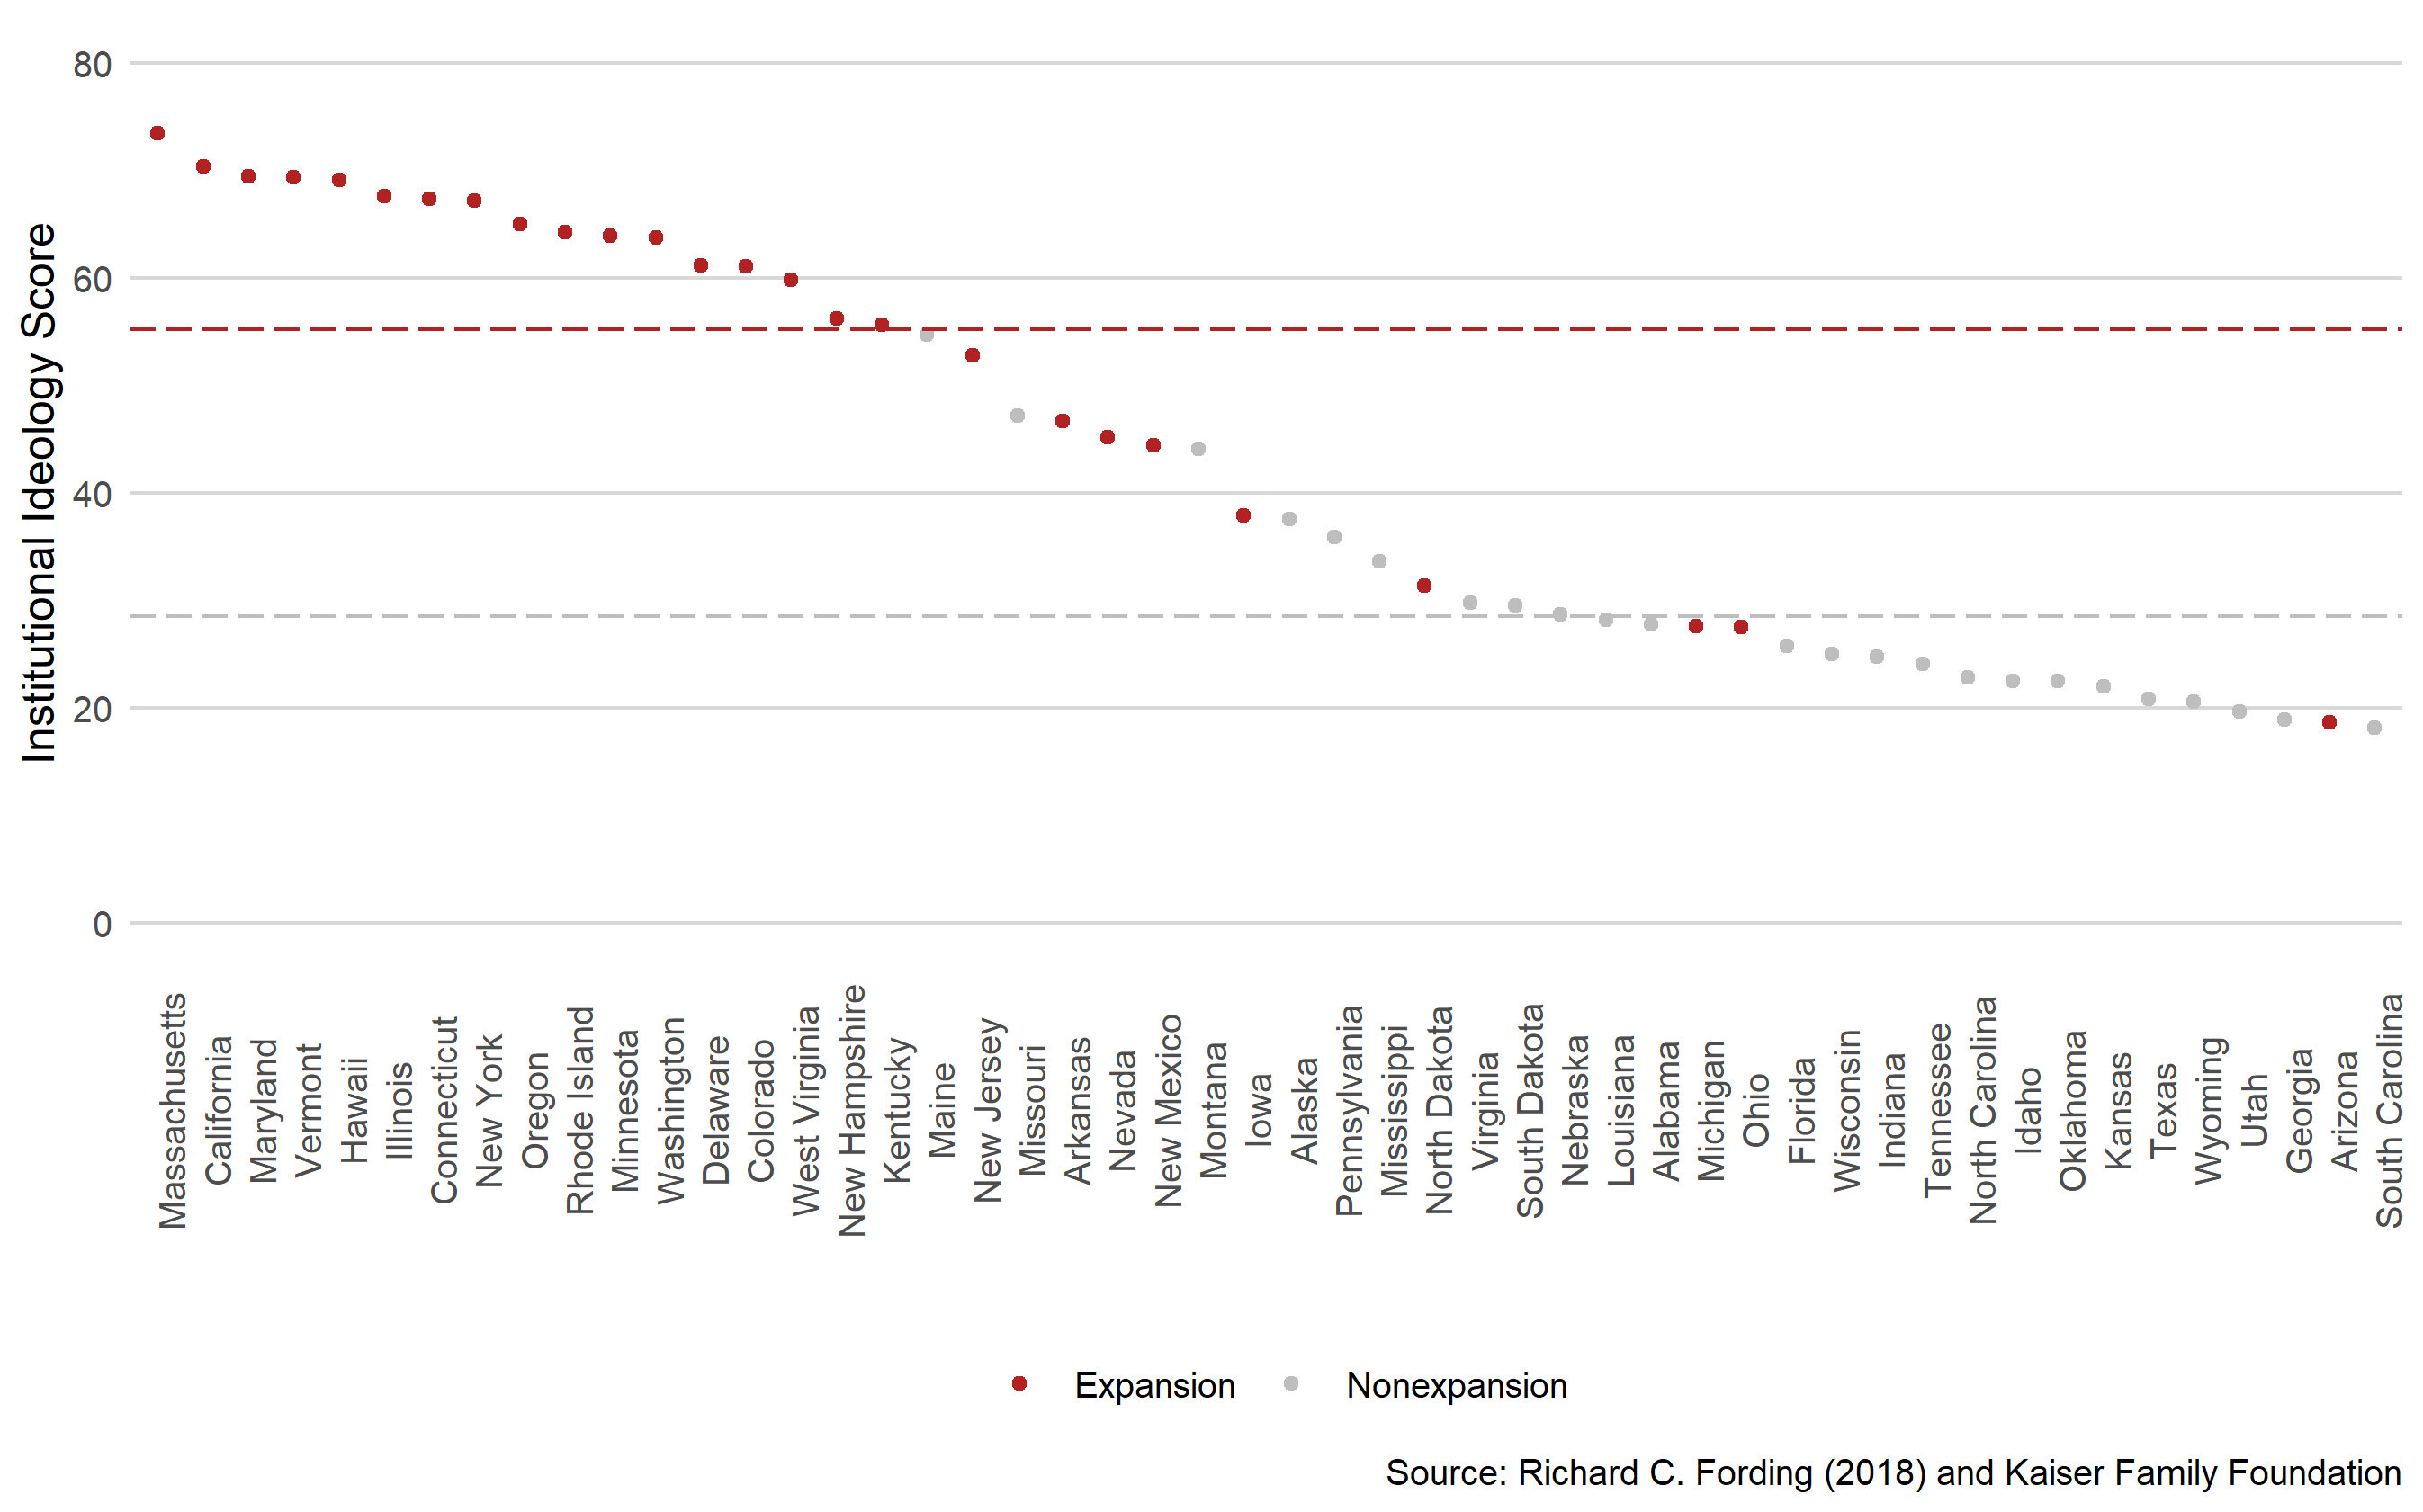
\includegraphics[scale=0.6]{01_Plots/political-expansion-plot.png}
    \end{center}
\end{figure}

This paper makes two methodological contributions to the literature on balancing weights. First, we extend the ``synthetic controls'' framework to estimate the treatment effect on the controls (ETC) using longitudinal data and we clarify the required assumptions. In brief, while balancing on pre-treatment outcomes alone arguably suffices for some synthetic control applications (see, e.g., \cite{botosaru2017role}), because our goal in this setting is to estimate treatment response, we must therefore balance on all covariates that predict treatment response, not just the outcome level absent treatment. Moreover, we cannot simply leverage pre-treatment data to conduct variable selection in this setting. We instead use an implementation of Stable Balancing Weights (\cite{zubizarreta2015stable}) to estimate a set of positive weights to weight the expansion regions to approximately match the covariate distribution of the non-expansion regions. 

Our second contribution is to modify the Stable Balancing Weights (SBW) objective function to account for our data, which is both hierarchical and has several covariates measured with error. Specifically, we use data from the American Community Survey (ACS) aggregated to the consistent public use microdata area (CPUMA) level. These regions nest within states, and using these smaller regions allows us to get better covariate balance. However, as a result, our data both has a hierarchical structure (regions within states) and, because our region-level covariates are estimated from underlying survey data, the sampling variability from our covariate estimates is a form of measurement error which may bias our treatment effect estimates. We first propose a modification of the SBW criterion to account for the hierarchical nature of the data, which disperses the weights more evenly across states. We then leverage the replicate survey weights provided in the ACS microdata to estimate the covariance matrix associated with the sampling variability and use this information to correct for this bias, following the regression calibration literature (see, e.g., \cite{gleser1992importance}). This is the first study we are aware of that attempts to adjust for hierarchical data structure and measurement error in the covariates when using balancing weights. 

The remainder of this paper has the following structure. Section 2 provides an overview of the data and defines the study period, covariates, outcome, and treatment. Section 3 discusses our methods, beginning by defining our target estimand, and then outlining our identification, estimation, and inferential procedures. Section 4 presents our results and sensitivity analyses. Section 5 contains a discussion of the policy relevance of our findings, and Section 5 contains a brief concluding summary of the paper. The Appendices contain additional materials, including summary statistics and additional results.

\section{Data}

In this section we overview of our data source, the covariates, the outcome, and the treatment assignment.

\subsection{Data Source}

Our primary data source is the annual household and person public use microdata files from the American Community Survey (ACS) from 2011 through 2014. The ACS is an annual survey of approximately three million individuals across the United States. The public use microdata files include information on individuals in geographic areas greater than 65,000 people. The smallest geographic unit contained in these data are public-use microdata areas (PUMAs), arbitrary boundaries that nest within states but not within counties or other more commonly used geographic units. One limitation of these data is a 2012 change in the PUMA boundaries, which do not overlap well with the previous boundaries. As a result, the smallest possible geographic areas that nest both PUMA coding systems are known as consistent PUMAs (CPUMAs). The United States contains 1,075 total CPUMAs, with states ranging from having one CPUMA (South Dakota, Montana, and Idaho) to 123 CPUMAs (New York). The average total number of sampled individuals per CPUMA across the four years within our primary dataset of 929 CPUMAs (discussed in Section \ref{sssec:txassign}) is 1,001; the minimum number of people sampled was 334 and the maximum is 23,990. Importantly, this survey does not follow specific individuals over time but rather reflects a different sample of individuals each year.

\subsection{Study period}

We begin our analysis in 2011 following \cite{courtemanche2017early}, who note that several other aspects of the ACA were implemented in 2010 -- including the provision allowing for dependent coverage until age 26, and the elimination of co-payments for preventative care -- and likely induced differential shocks across states. We also restrict our post-treatment period to 2014: several additional states expanded Medicaid in 2015, including Indiana, Michigan, and Pennsylvania. However, these states did not expand Medicaid contemporaneously with the 2014 ACA provisions. Without additional assumptions, this second-year expansion cannot help us estimate the effect of the 2014 expansion. 

\subsection{Covariates}

We use the underlying individual-level ACS survey data and accompanying survey weights to aggregate the data at the CPUMA level. We choose our covariates to approximately align with those considered in \cite{courtemanche2017early} and that are likely to be potential confounders. Because we are ultimately interested in calculating rates, these variables include both the numerator and denominator counts.\footnote{When viewing the denominator variables as random, these ratio estimators will in general be biased. This bias, however, decreases quickly with the sample size (is $O(n^{-1})$). Given that our CPUMA sample sizes are all over 300, we treat these estimates as unbiased in our analysis.}

Using the ACS survey weights, we first estimate: the total non-elderly adult population for each year 2011-2014; the total labor force population (among non-elderly adults) for each year 2011-2013; and the total number of households averaged from 2011-2013. We also construct an average of the total non-elderly adult population from 2011-2013. These are our denominator variables. For our numerator counts, we estimate the total number of: females; whites; people of Hispanic ethnicity; people born outside of the United States; citizens; people with disabilities; married individuals; people with less than a high school education, high school degrees, some college, or college graduates or higher; people living under 138 percent of the FPL, between 139 and 299 percent, 300 and 499 percent, more than 500 percent, and who did not respond to the income survey question; people aged 19-29, 30-39, 40-49, 50-64; households with one, two, or three or more children, and households that did not respond about the number of children.\footnote{Number of children and income to poverty ratio were the only two variables with missing data in the underlying microdata.} We average these estimated counts using the ACS survey weights from 2011-2013. For each individual year from 2011-2013, we estimate the total number of people who were unemployed and uninsured at the time of the survey (calculated among all non-elderly adults and all non-elderly adults within the labor force, respectively). We divide the numerator counts by the corresponding denominator counts to estimate the percentage in each category. For the demographics, these include the average number of non-elderly adults from 2011-2013. For the time-varying variables, we use the corresponding year (where uninsurance rates are calculated as a fraction of the labor force rather than the non-elderly adult population). We also calculate the 2011-2012 and 2012-2013 non-elderly adult population growth and the average number of households to adults across 2011-2013. 

In addition to the ACS microdata, we use 2010 Census data to calculate the approximate percentage of people living within an ``urban'' area for each CPUMA. Finally, we include three state-level covariates reflecting the partisan composition of each state's government in 2013. Specifically, we use data from the National Conference of State Legislatures (NCLS) to generate an indicator for states with a Republican governor, an indicator for states with Republican control over the lower legislative chamber, and an indicator for states with Republican control over both chambers of the legislature and the governorship.\footnote{Nebraska is the only state with a unicameral legislature; moreover, the legislature is technically non-partisan. We nevertheless classified them as having Republican control of the legislature.} 

\subsection{Outcome}

Our outcome of interest is the non-elderly adult uninsurance rate in 2014, which we denote using $Y$. While take-up among the Medicaid-eligible population is a more natural outcome, we choose the non-elderly adult uninsurance rate for two reasons, one theoretic and one practical. First, Medicaid eligibility in the post-period is likely endogenous: Medicaid expansion may affect an individual's income and poverty levels, which in general define Medicaid eligibility. A second reason is to align our study with others to compare our results with the existing literature, and this is the outcome that \cite{courtemanche2017early} use. One drawback of using this outcome is that the simultaneous adoption of other ACA provisions in 2014 more clearly affects this rate in a way that a more targeted group might not be.

\subsection{Treatment assignment} \label{sssec:txassign}

While some states expanded Medicaid and other states did not, assigning a binary treatment status simplifies a more complex reality. There are three reasons to be cautious about this simplification. First, states differed substantially in their Medicaid coverage policies prior to 2014: with perfect data we might consider Medicaid expansion as a continuous treatment with values proportional to the number of newly eligible individuals. The challenge though is correctly identifying newly eligible individuals in the data (see \cite{frean2017premium}, who attempt to address this). Second, \cite{frean2017premium} note that five states (California, Connecticut, Minnesota, New Jersey, and Washington) and the District of Columbia adopted partial limited Medicaid expansions prior to 2014. \footnote{\cite{kaestner2017effects} and \cite{courtemanche2017early} also consider Arizona, Colorado, Hawaii, Illinois, Iowa, Maryland, and Oregon to have had early expansions.} Lastly, timing is an issue: among the states that expanded Medicaid in 2014, Michigan's expansion did not go into effect until April 2014, while New Hampshire's expansion did not occur until September 2014.

Our primary analysis excludes New York, Vermont, Massachusetts, Delaware, and the District of Columbia from our pool of expansion regions, because these regions had comparable Medicaid coverage policies prior to 2014 (\cite{kaestner2017effects}). We also exclude New Hampshire because it did not expand Medicaid until September 2014. While Michigan expanded Medicaid in April 2014, we leave this state in our pool of treated states. We consider the remaining expansion states as ``treated'' and the non-expansion states as ``control'' states. We later consider the sensitivity of our results to these classifications by removing the early expansion states noted by \cite{frean2017premium}. Our final dataset contains aggregated statistics for all of the above variables for 925 CPUMAs in our non-expansion and our pool of expansion states. There are 414 CPUMAs among 24 non-expansion states and 515 CPUMAs among 22 expansion states. When we exclude the early expansion states for sensitivity analyses, we are left with 296 CPUMAs across 17 states.

\section{Methods}
\label{sec:methods}

In this section we present our causal estimand, identifying assumptions, estimation strategy, and inferential procedure.

\subsection{Estimand}

Our goal is to estimate the average effect 2014 Medicaid expansion would have had on the non-elderly adult uninsurance rate in states that did not expand Medicaid. Let $c$ index a CPUMA, $s$ index the state, and $t$ index the time period. Let $N_1$ be the number of treated CPUMAs, $N_0$ be the number of control CPUMAs, and $N$ be the total number of CPUMAs. Similarly, let and $M = M_1 + M_0$ states (with $M_1$ and $M_0$ defined analogously). Each state has $n_s$ CPUMAs. Since we are only interested in the counterfactual at time $T = 2014$, we simplify notation by removing this variable and the subscript and write our formal estimand as:

$$
\psi = \psi^1 - \psi^0 = N_0^{-1}\sum_{s, c: A_s = 0} Y_{sc}^{A_s = 1} - Y_{sc}^{A_s = 0}
$$

We observe $\psi^0$ in the data; the challenge is estimating $\psi^1$ using our pool of treated units. That is, we wish to predict the counterfactual uninsurance rates in 2014 for states that did not expand Medicaid expansion had they expanded their Medicaid eligibility requirements. \foonote{The 2014 Medicaid expansion occurred simultaneously with the implementation of several other major ACA provisions, including (but not limited to) the creation of the ACA-marketplace exchanges, the individual mandate, health insurance subsidies, and community-rating and guaranteed issue of insurance plans (\cite{courtemanche2017early}). Almost all states broadly implemented these reforms beginning January 2014. Conceptually we think of the other ACA components as a state-level treatment ($V$) separate from Medicaid expansion ($A$). Therefore, our total estimated effect may also include interactions between these policy changes; however, we do not attempt to separately identify these effects. Because the ACA implementation and Medicaid expansion may vary over time, we do not try to generalize these results beyond 2014.} 

\subsection{Identification}

The following causal assumptions are necessary (though not sufficient) to enable us to identify our target parameter from the data: consistency, no unmeasured confounding, no anticipatory treatment effects, and positivity of treatment assignment. We explain these assumptions in detail and their consequences below. We additionally invoke several parametric assumptions to help us identify our causal parameter given the measurement error in our covariates.

Consistency states that the observed factual outcome under a given treatment assignment is equal to the potential outcome under that same treatment assignment ($Y_{sc}^{A_{sc} = a} = Y_{sc} \mid A_{sc} = a$). In other words, we assume that one region's treatment assignment does not affect another region's observed outcome. This is a standard assumption, but is often not realistic. Violations of this assumption are likely in our setting: for example, \cite{frean2017premium} find evidence that Medicaid expansion drove previously eligible but uninsured individuals to enroll in Medicaid in both expansion and non-expansion states. Signing the potential bias from this violation requires redefining the causal estimand: for example, we might consider the treatment effect on the untreated given that all states have expanded Medicaid, where the contrast is against where only the observed expansion states expanded Medicaid. If spillovers occurred in equal proportions across each region, and the magnitude of the spillovers increase with the total number of treated regions, then the true effect would be larger in absolute magnitude than the estimated estimated using the observed data. We could consider other estimands or assumptions to get different predictions about the sign of the bias; however, this is beyond the scope of this paper.

We next assume that there were no anticipatory treatment effects. Letting treatment occur at time $T$, we have that for $t < T$:

$$
Y_{sct} = Y_{sct}^0
$$

This assumption is necessary because we are conditioning on pre-treatment outcomes. If these outcomes were affected by the treatment before it were implemented, these covariates would be endogenous. Anticipatory treatment effects may occur if plans to expand Medicaid induce uninsured but Medicaid-eligible individuals to enroll in Medicaid prior to expansion. We do not think these violations occurred in large enough numbers to substantially affect our results. Instead, we address a more concerning version of this violation: the fact that several states allowed certain counties to expand Medicaid prior to 2014. We therefore test the sensitivity of our results to the exclusion of these states.

Third, we assume no unmeasured confounding; that is, that at time $T$ the potential outcomes for each CPUMA are independent of the state-level treatment assignment conditional on the population-level CPUMA and state-level covariates $X_{sc}$ (which includes pre-treatment outcomes):

$$
Y_{sc}^a \perp A_{sc} \mid X_{sc}
$$

While unverifiable, we believe it is reasonable here given our rich covariate set. To be explicit, we believe that the potential uninsurance rates for each CPUMA are independent of the treatment assignment conditional on the percentage of uninsured individuals in each year of the pre-treatment period, the percentage of unemployed individuals in each year of the pre-treatment period, the population growth in 2012 and 2013, the average ratio of households to non-elderly adult population, the state's political composition, the average proportion of households with one, two, or three or more children during the pre-treatment period, the average proportion of households who did not respond about their number children, and the average proportion of individuals during the pre-treatment period with given demographics noted above (age group, sex, white, Hispanic ethnicity, U.S. citizenship, foreign born, income-to-poverty group (including non-response), disability status, urban residence, and educational attainment group). 

Finally, we assume positivity of treatment assignment; that is, that all states had some non-zero probability of being treated $\pi(X_{1s}, ..., X_{n_ss}) > 0$. Positivity violations can cause a lack of covariate overlap in the observed data. Overlap is an issue in this study. We address this in multiple ways that we outline in our estimation strategy below. 

These assumptions are sufficient to non-parametrically identify our causal estimand if we observed the true covariates $X_{sc}$. Unfortunately, for our covariates estimated using the ACS data, we do not observe the true values of $X_{sc}$ but rather a mean-unbiased estimate $W_{sc}$. Importantly, $Y_{sc}^a \perp A_{sc} \mid X_{sc} \centernot\implies Y_{sc}^a \perp A_{sc} \mid W_{sc}$. The use of these proxies may also bias our estimates; we therefore rely on several modeling assumptions to correct for this bias.

First, we assume that the potential outcome under treatment is linear in the covariates $X_{sc}$. Specifically, we assume that the following model generates the potential non-elderly adult uninsurance rate under treatment:

$$
Y_{sc}^1 = \alpha + X_{sc}^T\beta + \epsilon_{sc} + c_s
$$

We assume that the errors $\epsilon_{sc}$ and $c_s$ are independent from each other and across time (i.e., we rule out serial-correlation), and that these errors are invariant to the intervention. This model then allows us to identify $\psi^1$ in terms of our model parameters; specifically, we have that $\psi^1 = \alpha + \bar{X}_0^T\beta$, where $\bar{X}_0$ is the (observed) mean covariate values among the control units.\footnote{To be precise, we use the population-weighted mean so as to target the individual-level treatment effect rather than the CPUMA-average treatment effect.} 

A classical assumption in the measurement-error literature is that $X$ and $W$ are jointly normally distributed, the measurement errors are independent and identically distributed, and these errors are uncorrelated with the outcome. Under these assumptions, it is well-known that standard regression-based estimates of $\beta$ will suffer from the following bias:

$$
\mathbb{E}\{\hat{\beta}\} = \kappa \beta
$$

where $\kappa = \Sigma_{WW \mid A = a}^{-1}\Sigma_{XX \mid A = a}$. Our causal parameter is a function of $\beta$, which is estimable from the data if we know (or can estimate) $\kappa$ (\cite{gleser1992importance}). Under these assumptions, our target parameter is identified.

In Appendix A we show that under the classical errors-in-variables model, the asymptotic bias for the SBW estimator that sets $\delta = 0$ is equivalent to the bias of a linear combination of coefficient estimates from the OLS-based regression estimator. The intuition for this result is as follows: exact balancing weights estimate an implicit $\beta$ on a subset of the data where we have sufficient overlap. We can therefore think of SBW as returning a solution to some implicit weighted-least squares problem. If we assume that the outcome model holds across all of the data, WLS and OLS are estimating the same $\beta$; therefore, the bias that effects the least squares solution will have the same effect on the WLS, and therefore SBW, solution. Our target parameter is therefore identified under the same conditions regardless of the estimation strategy.

For this application we make a slight departure from the classical setting, assuming that that $W_{sc} = X_{sc} + v_{sc}$, where $\sqrt{s_{sc}}v_{sc}$ are drawn iid from $MVN(0, \Sigma_{vv \mid A = a})$, and where $s_{sc}$ are the vector of sample sizes used to calculate $W_{sc}$. We again assume that $v_{sc}$ is independent of the CPUMA-level errors $\epsilon_{sc}$ (which may include measurement error in the outcome) and the state-level errors $c_s$. We believe this is reasonable because the errors in the CPUMA-level aggregates are estimated from a 2014 cross-section of individuals, while the covariates are estimated from different individuals surveyed from 2011-2013. \footnote{While the sample sizes for each CPUMA are all relatively large, the variance is still larger than one might expect due to the design effect of the survey.} 

\subsection{Estimation}

We outline our estimation strategy first emphasizing how our method differs from the synthetic controls approach, which motivates our use of the SBW objective. Second, we explain a modification we make to the SBW criterion to address the hierarchical data structure (which we call H-SBW) that reduces the variance of our estimator under our assumption of within-state correlation of our model errors. Third, we connect our estimator to the regression calibration literature by generating weights that balance a linear prediction of the true covariates $\hat{\eta}_a(W_{sc})$ using the observed covariates $W_{sc}$. 

We also test the sensitivity of our estimator to a ridge-augmented version, following the suggestion of \cite{ben2018augmented}; this allows us to achieve better covariate balance by extrapolating beyond the support of the data. As a separate sensitivity check, we estimate a different causal parameter -- the overlap average treatment effect (OATE) -- using overlap weights, as discussed in \cite{li2018balancing}. Estimating this effect does not require extrapolation, but rather changing the target estimand. We discuss this further below.

Similar to synthetic controls applications, we seek to generate a set of positive weights that balance the means of covariates for the treated units to the mean of covariates for the control units. Assume that we observe the true covariate matrices $X_1$ and $X_0$, and let $\bar{X}_0$ be the (population-weighted) average of the covariate values in the non-expansion region. Ideally, we could then find some $\gamma^\star$ such that for $\delta = 0$: 

$$
(\frac{1}{N_0}X_1^T\gamma^\star - \bar{X}_0) \le \delta, \gamma_i^\star > 0, \sum_{sc} \gamma_{sc}^\star = N_0
$$

Let $p$ be a vector of (normalized) population weights for each CPUMA in the non-expansion region in year $T = 2014$. We could then estimate $\psi$ as

$$
\hat{\psi} = (N_0^{-1}\sum_{s: A_s = 1}^{M_1}\sum_{c = 1}^{n_s}\gamma_{sc}^\star Y_{sc} - \sum_{s: A_s = 0}\sum_{c = 1}^{n_s}Y_{sc}p_{sc})
$$

The assumption that the outcomes (absent treatment) follow a linear factor model frequently motivates the synthetic controls approach; here we instead assume no unobserved confounding and assume that the outcomes given treatment are a linear function of the covariates: $\mu_1(X_{sc}) = \alpha + X_{sc}^T\beta$. The bias of our estimator (again assuming we observed $X_{sc}$), is therefore less than or equal to $\lvert\beta\rvert^T\delta = 0$ (see, e.g., \cite{zubizarreta2015stable}). The challenge, however, is that for any given dataset we have no guarantee that any such $\gamma$ exists that exactly balances the covariates; we therefore need some method of determining how to prioritize which parts of the covariate distribution we wish to balance to minimize this bias.

This is where estimating the ETC contrasts with the commonly used synthetic control approach used to estimate the ETT: \cite{abadie2010synthetic} determine how to prioritize covariate balance by training their model on pre-treatment outcomes (\cite{kaul2015synthetic} shows that often the most relevant covariates simply become the pre-treatment outcomes). Because in that setting the counterfactual value $Y^0_{sct}$ is actually observed for $t \le T_0$, \cite{abadie2010synthetic} are able to leverage this data to select the covariates that best predict these values. By contrast we never observe $Y^1_{sct}$ prior to treatment. Without additional assumptions, we cannot use the pre-treatment data to learn which covariates matter most for determining this potential outcome.

Moreover, the problem of predicting treatment response also makes estimating the ETC more challenging to estimate than the ETT. In particular, we likely care more about balancing ``auxillary covariates'' (covariates that are not pre-treatment outcomes) in our setting than the traditional synthetic controls setting. To see this, assume that $\mu_0$ is linear in the covariates, including the pre-treatment outcomes. We might reasonably believe the coefficients on the auxillary covariates are close to zero once we condition on pre-treatment outcomes. As a result, the bias induced by remaining imbalances on the auxillary covariates would be small. On the other hand, assuming $\mu_1$ is also linear in the same covariates, the coefficients on this model could be much larger, even after conditioning on pre-treatment outcomes, because these coefficients are highly predictive of treatment response. If our weights fail to balance these covariates, we should expect that our estimates of $\mu_0$ will in general have less bias than our estimates of $\mu_1$. In summary, estimating the ETC requires a greater understanding of how the covariates are related to treatment response than the ETT; moreover, we cannot learn this information by using pre-treatment outcomes.

We therefore estimate the ETC by using a variation of SBW that we call H-SBW.\footnote{Specifically, we use a modified implementation of Noah Griefer's ``optweight'' package in R, available on github.com/mrubinst757} This procedure allows us to estimate the minimum variance weights that satisfy user-specified balance constraints. Let $\eta_a(W_{sc}) = \mathbb{E}\{X_{sc} \mid W_{sc}, A_s = a\}$, and $\hat{\eta}_1(W_1)$ be a matrix of estimates of $\eta_1(W_1)$. Let $\bar{W}_0$ be a vector of population-weighted estimates of the covariates for the non-expansion region.\footnote{Because $\bar{W}_0$ and $\bar{X}_0$ are equal in expectation, the use of this target will not contribute to any asymptotic bias of our estimator.} We generate weights that solve the following objective:

$$
\min_{\gamma \in \Gamma} \sum_{s: A_s = 1}^{M_1}(\sum_{c = 1}^{n_s} \gamma_{sc}^2 + \sum_{c \ne d}\rho \gamma_{sc}\gamma_{sd})
$$

$$
\Gamma := \{\gamma \mid \frac{1}{N_0}\hat{\eta}_1(W_{sc})^T\gamma - \bar{W}_0 \mid \le \delta, \gamma_{sc} > 0, \sum_{sc}\gamma_{s,c} = N_0\}
$$

This objective is a modification of the SBW objective, which sets $\rho = 0$ and balances on $W_{sc}$ rather than $\eta_1(W_{sc})$. Importantly, both allow the user to specify covariate-level balance constraints using the vector $\delta$. When estimating the ETC, we lean heavily on assumptions to justify our choice of $\delta$; in particular, we use a priori domain knowledge about which covariates are most likely to be important predictors of treatment effect heterogeneity when setting $\delta$. However, we also must choose $\delta$ to something that is feasible given the data. 

For our application, we constrain $\delta$ to be 0.05 percentage points for pre-treatment outcomes, 0.1 percentage points for pre-treatment unemployment rates. We believe these are the most likely factors associated with treatment response, so we prioritize balancing these covariates. For the remaining covariates, we let $\delta$ be 0.25 percentage points for population growth, 1 percentage point for female, Hispanic ethnicity, white race, age category, disability, and number of children category; 2 percentage points for urban, citizenship, education category, income-to-poverty category, student, and foreign-born; and 20 percentage points for the Republican governance indicators. We choose these constraints primarily on feasibility concerns, and for our variance estimates, we reduce these initial constraints when this constraint set becomes infeasible.

We now discuss how H-SBW differs from SBW, beginning with the criterion. The motivation of the SBW criterion, which is equivalent to ours with $\rho = 0$, is to produce the minimum variance weights for a fixed $\delta$. This produces the minimum variance estimator within the constraint set if, for example, the errors in the outcome model are independent and identically distributed. In our setting we have possible state-level dependencies, reducing the efficiency of the SBW estimator. To improve the efficiency, we add the tuning parameter $\rho$; this parameter attempts to more uniformally disperse the weights across states. This objective produces the minimum variance estimator within the constraint set if we assume a constant (and known) within-state correlation of the errors ($\rho$) and constant variance across units. We discuss this objective in more detail and provide simulation results in Rubinstein et al. (2021) (pre-print not yet available); broadly speaking, we can think of H-SBW being to SBW what generalized least squares (GLS) is to ordinary least squares (OLS): both SBW and OLS can produce unbiased estimates of model parameters; however, H-SBW and GLS can produce efficient estimators assuming a block-matrix correlation structure in the outcome errors. 

A second departure from SBW comes in the constraint set: rather than balancing on the observed covariate values $W_{sc}$, we instead balance on our estimate of $\eta_1(W_{sc})$. This is because the estimation error in these CPUMA-level covariates will bias our estimate of $\psi^1$. In Appendix A we show that if we had access to $\eta_1$, we could obtain an unbiased estimate of the super-population parameter $\psi^1 = \mathbb{E}\{Y_i^1 \mid A_i = 0\}$ by balancing on $\eta_1(W_{sc})$.\footnote{For the finite-sample parameter we're interested in here, the estimator will have some finite-sample bias.} In practice we do not know $\eta_1$ but must estimate it using auxillary data. Here we leverage the person-level replicate survey weights provided in the ACS microdata to estimate the variability in each CPUMA's observed covariate values. We then use a variant of regression calibration techniques to estimate $\eta_a(W_{sc})$ as a linear approximation to the true covariate values (see, eg, \cite{gleser1992importance}, \cite{carroll2006measurement}). We consider two versions of this procedure: first, our preferred version which accounts for the fact that some covariates are estimated much more precisely than others, but that assumes that all of the differences in the errors are attributable to the different sample sizes used to estimate the covariates. This allows us to generate a separate $\kappa$ for each unit. We then generate a second adjustment that follows the traditionally used procedures in this setting which does not account for this differential precision, and instead averages over all observed variance estimates to estimate a single $\kappa$ for all units. Further details about these covariate adjustment procedures are available in Appendix B.

This is the first application we are aware of to use regression calibration methods in the context of balancing weights. We emphasize two critical assumptions for using this procedure in our context: (1) the outcome model is linear in the true covariates; and (2) the measurement error in the outcome is unrelated to the measurement error in the covariates. The first assumption is strong, though often used in practice. The second assumption is reasonable, because our outcomes are estimated from a different cross-section of individuals than our covariates. 

Lastly, we are unable to achieve exact balance, which may also contribute to the bias of our estimator. Following the recent literature on synthetic controls, we test the sensitivity of our results to these imabalances by using ridge-regression augmented weights \cite{ben2018augmented}. Letting $\hat{\eta}_1(W_1)$ be the matrix of adjusted covariates, and $\gamma^{hsbw}$ be our H-SBW weights, we standardize our weights to sum to one and estimate the regression-augmented weights:

$$
\gamma^{aug} = \gamma^{hsbw} + (\hat{\eta}_1(W_1)^T\gamma^{hsbw} - \bar{W}_0)^T(\hat{\eta}_1(W_1)^T\Omega^{-1}\hat{\eta}_1(W_1) + \lambda I_d)^{-1}\hat{\eta}_1(W_1)^T\Omega^{-1}
$$

where $\Omega$ is a block diagonal matrix with diagonal entries equal to one and the within-group off diagonals equal to $\rho$. We choose $\lambda$ so that the remaining imbalances all fall within 0.1 percentage points (see \cite{ben2018augmented} for more details on the connection between these weights and ridge-regression). The cost of this procedure is that we must extrapolate from the support of the data, and therefore rely more heavily on our modeling assumptions. In our results we consider estimators using SBW ($\rho = 0$), H-SBW ($\rho = 0.2$), and ridge-augmented versions of SBW and H-SBW that we call BC-SBW and BC-HSBW. We focus our discussion on our preferred estimator, H-SBW, and its ridge augmented version BC-HSBW. 

Our secondary research hypothesis is that conservative governance moves the estimated treatment effect towards zero. We examine this by removing the Republican governance indicators from the covariate set and recalculating our point estimates and comparing this estimated contrast to our original point estimate (i.e., the estimated treatment effect when all covariate groups are included). This difference is a function both of the model coefficients and the differences in the weighted imbalances between the covariates of the treated and control groups.

More formally, let $\hat{\psi}_v$ be the estimator with covariates $V \subset X$ removed using weights $\gamma_v$; let $\beta_v$ be the model coefficients on those covariates; and let $\hat{\psi}^1_0$ be our primary estimator. This procedure approximately estimates the following quantity:\footnote{Notice that these final two lines are approximations rather than equalities for four reasons: one, error in the outcome model; two, estimation error from $\hat{\eta}(W_{sc})$; three, the difference between $\eta(W_{sc})$ and $X_{sc}$; and finally, because while we hold $\delta$ constant for all covariates not in $V$, the reweighting may affect the imbalances within that error tolerance for non-binding constraints.}

\begin{align*}
    \hat{\Delta}_v &= \hat{\psi}_v - \hat{\psi}_0 \\
    &= (\hat{\psi}^1_v - \hat{\psi}^0_1)  - (\hat{\psi}^1_0 - \hat{\psi}^1_0) \\
    &= \hat{\psi}^1_v - \hat{\psi}^1_0 \\
    &\approx (X_1^T(\gamma_v - \gamma_0))^T\beta \\
    &\approx (V_1^T(\gamma_v - \gamma_0))^T\beta_v
\end{align*}

Because we hypothesize that regions under Republican-governed administrations will have lower Medicaid take-up rates, we expect that removing these covariates will move the point estimate farther away from zero, controlling for all other factors. Specifically, for these covariates we know that $V_1^T(\gamma_1 - \gamma_0)$ will be negative because the treated region is much more Democratic than the control region. Because we expect that Republican governance is positively associated with uninsurance rates, our hypothesis is that this overall quantity will be negative. We also examine the influence of four other covariate groups: pre-treatment uninsurance rates and pre-treatment unemployment rates, and three sets of different demographic indicators. Specifically, the first group includes: urban residence, age group, education, citizenship, student, disability, female; the second, white race, Hispanic ethnicity, foreign-born, and income-to-poverty ratio; the third, children category (0, 1, 2, 3+, NA), household to population ratio, and population growth; however, we leave the presentation of these results to Appendix E.

\subsection{Inference}

We estimate $Var(\hat{\psi} \mid W)$ by decomposing this estimator into two parts: $Var(\hat{\psi}^1 \mid W) + Var(\hat{\psi}^0 \mid W)$. We view the unobserved covariates $X$ as fixed so that the randomness of our estimator is a function of (1) the errors in our outcome model; (2) our estimator $\hat{\eta_1}_1$.\footnote{Assuming $\hat{\eta}_a$ is unbiased for $\eta_a$, the remaining differences $\hat{\psi} - \psi$ are a function of $X_{sc} - \eta_1(W_{sc})$ which lead to a finite-sample bias; see Appendix A.} We use the leave-one-state-out jackknife to estimate the variance $Var(\hat{\psi}^1 \mid W)$ (\cite{cameron2015practitioner}), where we hold our reweighted targets fixed at $\bar{W}_0$, which are an unbiased estimate of $\bar{X}_0$. When our preferred choice of $\delta$ does not converge, we programmatically reduce the constraints until the optimization program reaches a solution. 

Our preferred estimator calculates this estimate conditioning on our covariate adjustment $\hat_1{\eta}(W_{sc})$. As a secondary estimate, we additionally recalculate $\hat{\eta_1}$ omitting each state in the jackknife procedure; however, we believe this estimator will be overly conservative. Since we view both $X$ and $W$ as fixed, the variability in $\hat{\eta}_1$ comes from the auxillary data used to calculate $\hat{\Sigma}_{vv}$. Unfortunately there is no simple way to re-sample from the underlying microdata to approximate the variability of this estimator. The jackknife procedure instead treats the uncertainty as coming from resampling $(X, W)$ from a larger super-population, and therefore gives an overly conservative variance estimate. Finally, we estimate $Var(\hat{\psi}^0 \mid W)$ using an auxillary regression model and take the variance of the linear combination $\bar{W}_0^T\beta$, using standard errors clustered at the state-level. Obtaining more precise inference in this setting is an interesting area that we leave for future work.

\section{Results}

This section presents the results from our analyses. We begin by presenting statistics on the imbalances in the covariates between the treatment, control, and weighted treatment groups. We then present our primary results, including both our treatment effect estimates and our analysis of the association of Republican governance on our estimates. We conclude by reviewing a series of sensitivity analyses that check the robustness of our results to using an alternative dataset and target estimand.

\subsection{Covariate Balance}

Figure~\ref{fig:loveplotc1} shows how our balancing weights reduce the imbalances among covariates with greater than one percentage point difference between the targeted mean in the expansion region and the mean values in the non-expansion region (we target the population-weighted mean of the untreated region).\footnote{The reweighted treatment values use our preferred covariate adjustment $\hat{\eta}_1(W_{sc})$.} Before applying our weights, we see that there are substantial imbalances in the Republican governance indicators, as well as pre-treatment uninsurance and unemployment rates. Our weights drastically reduce these differences; however, some imbalances remain. In particular, imbalances remain in the Republican governance indicators. A complete balance table is available in Appendix D, Table~\ref{tab:baltab1}. Appendix C contains additional summary statistics. 

\begin{figure}[B]
\begin{center}
    \caption{Balance plot, primary dataset}
    \label{fig:loveplotc1}
    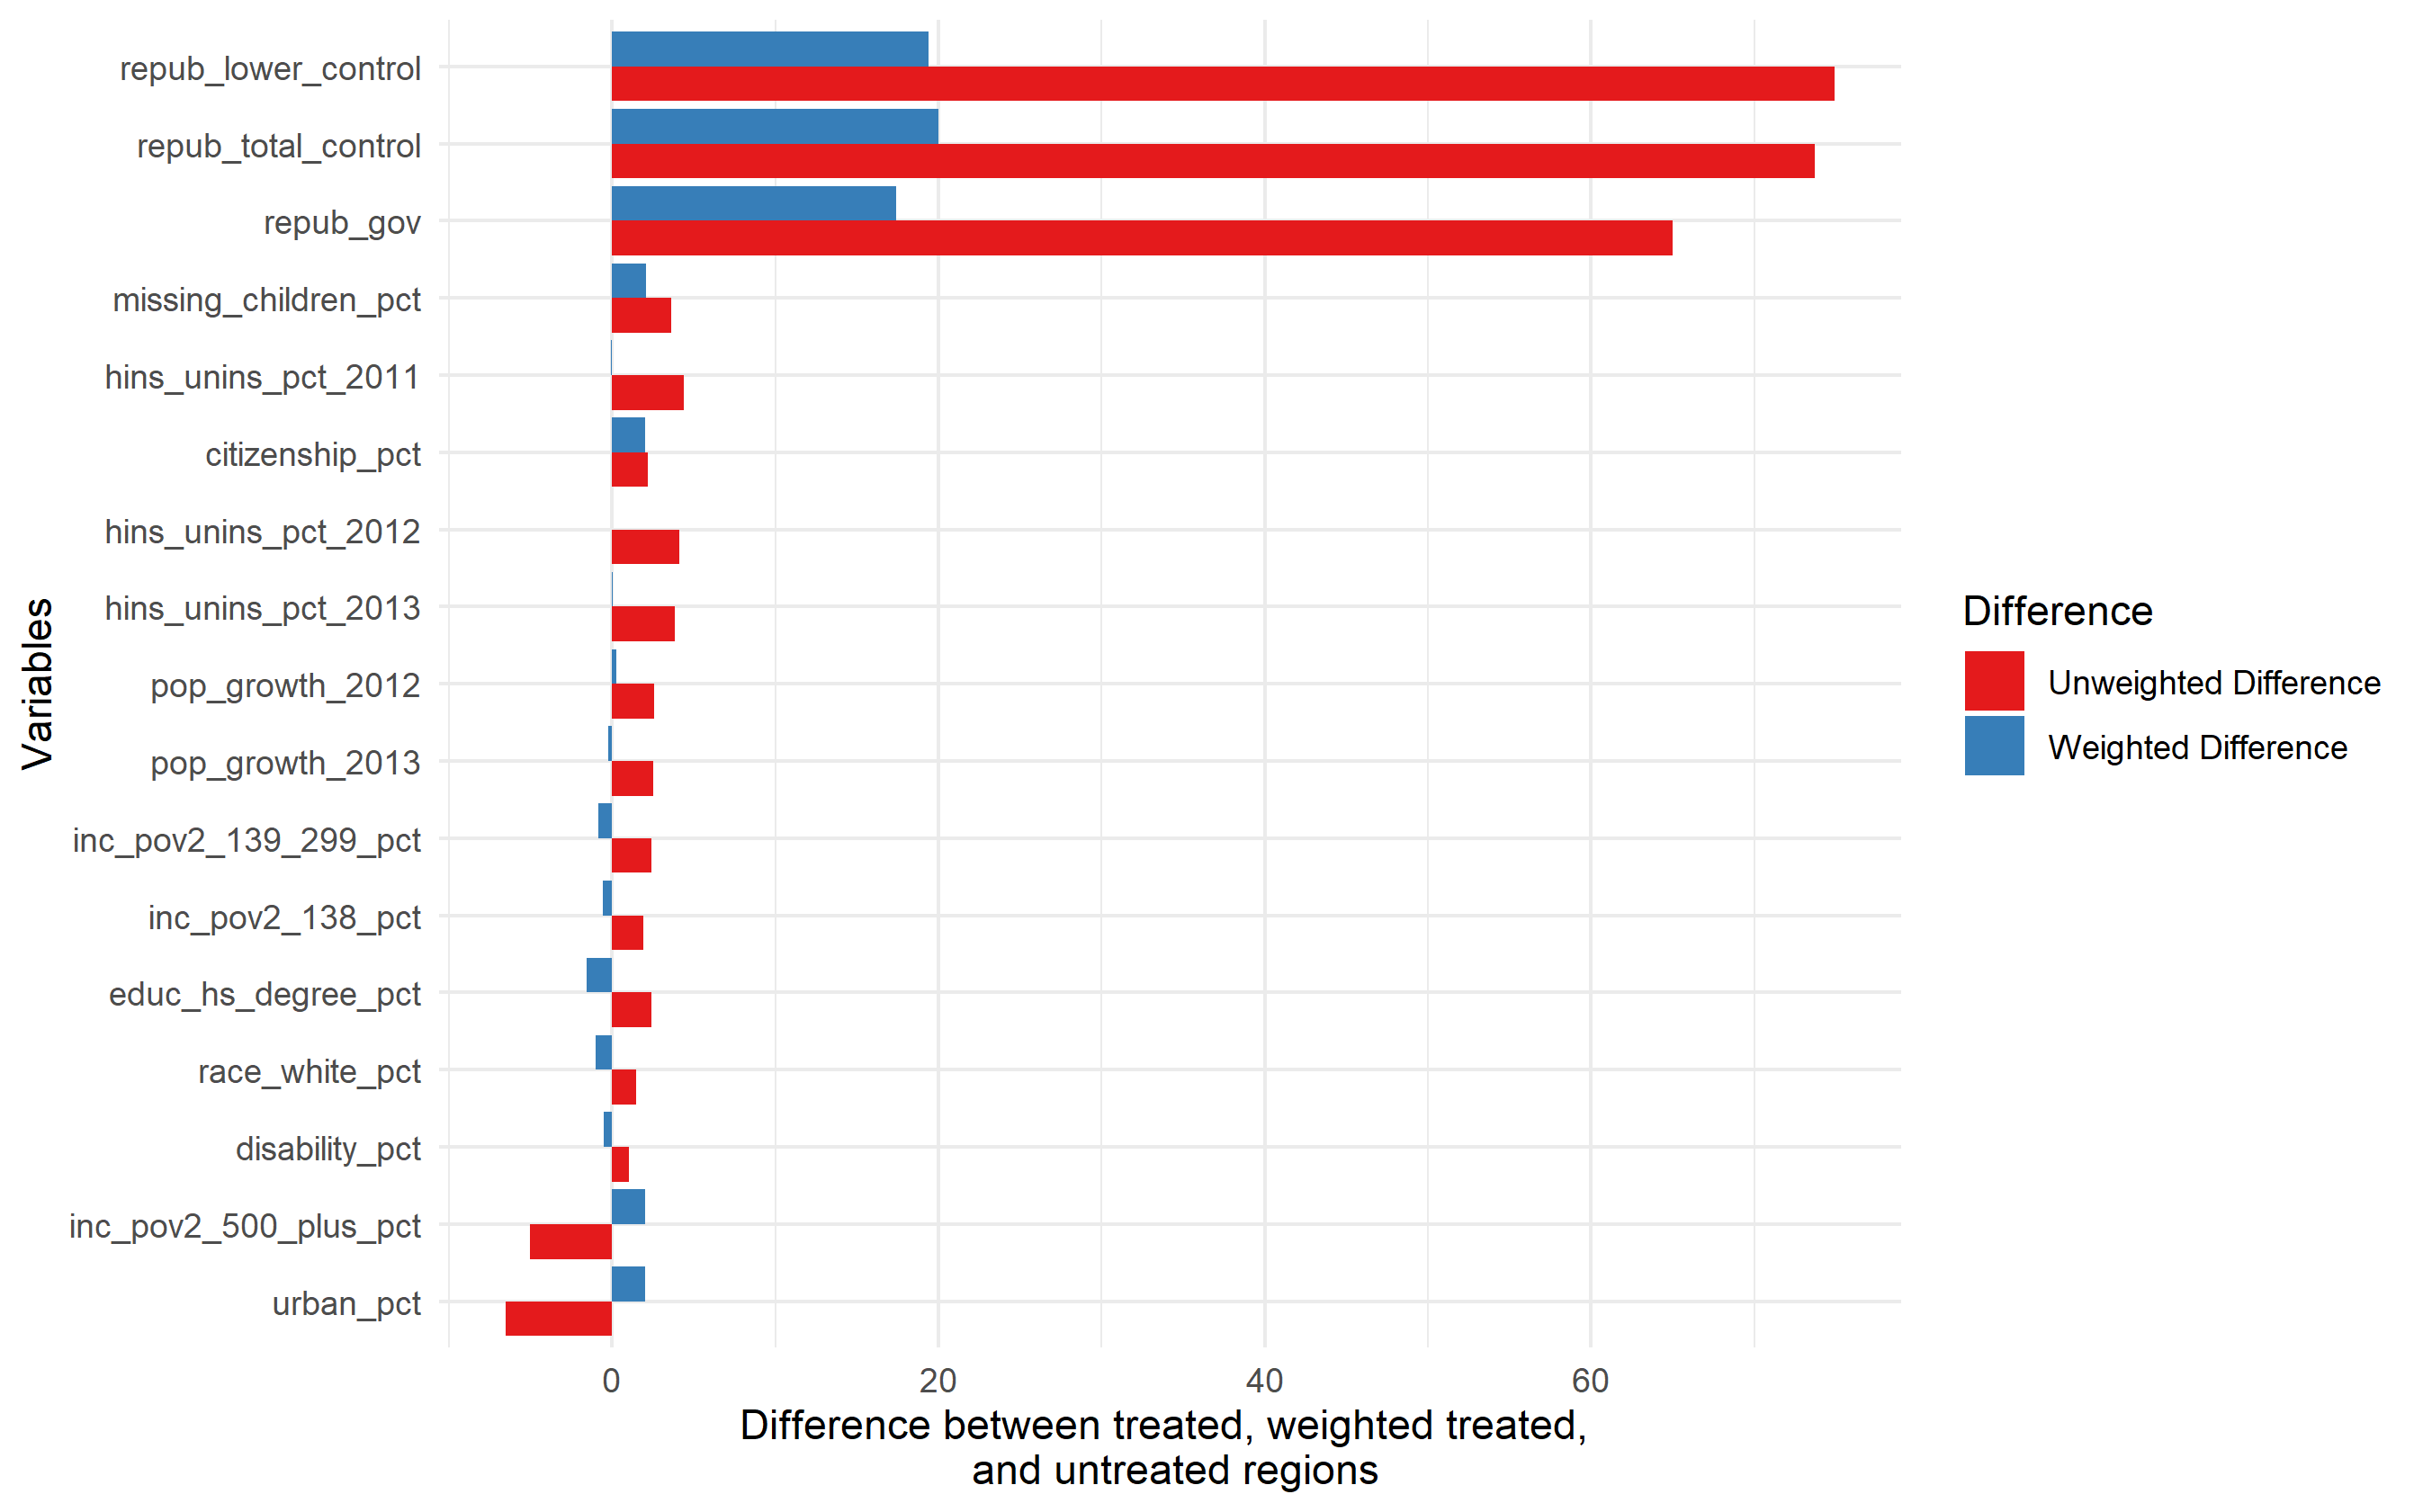
\includegraphics[scale=0.6]{01_Plots/balance-plot-etu.png}
\end{center}
\end{figure}

As discussed above, we use a ridge-regression augmentation to extrapolate from the data in order to reduce all imbalances within 0.1 percentage points. Figure~\ref{fig:statewghts} shows the total weights summed across states for each estimator: H-SBW and BC-HSBW. This figure sums the negative weights separately from the positive weights to show the extent of the extrapolation. We see that BC-HSBW extrapolates heavily in order to estimate the counterfactual, particularly for CPUMAS in California. Due to this extensive extrapolation, we therefore prefer the H-SBW estimator, though we compare results against BC-HSBW as a robustness check.

\begin{figure}[B]
\begin{center}
    \caption{Total weights summed by state, primary dataset}
    \label{fig:statewghts}
    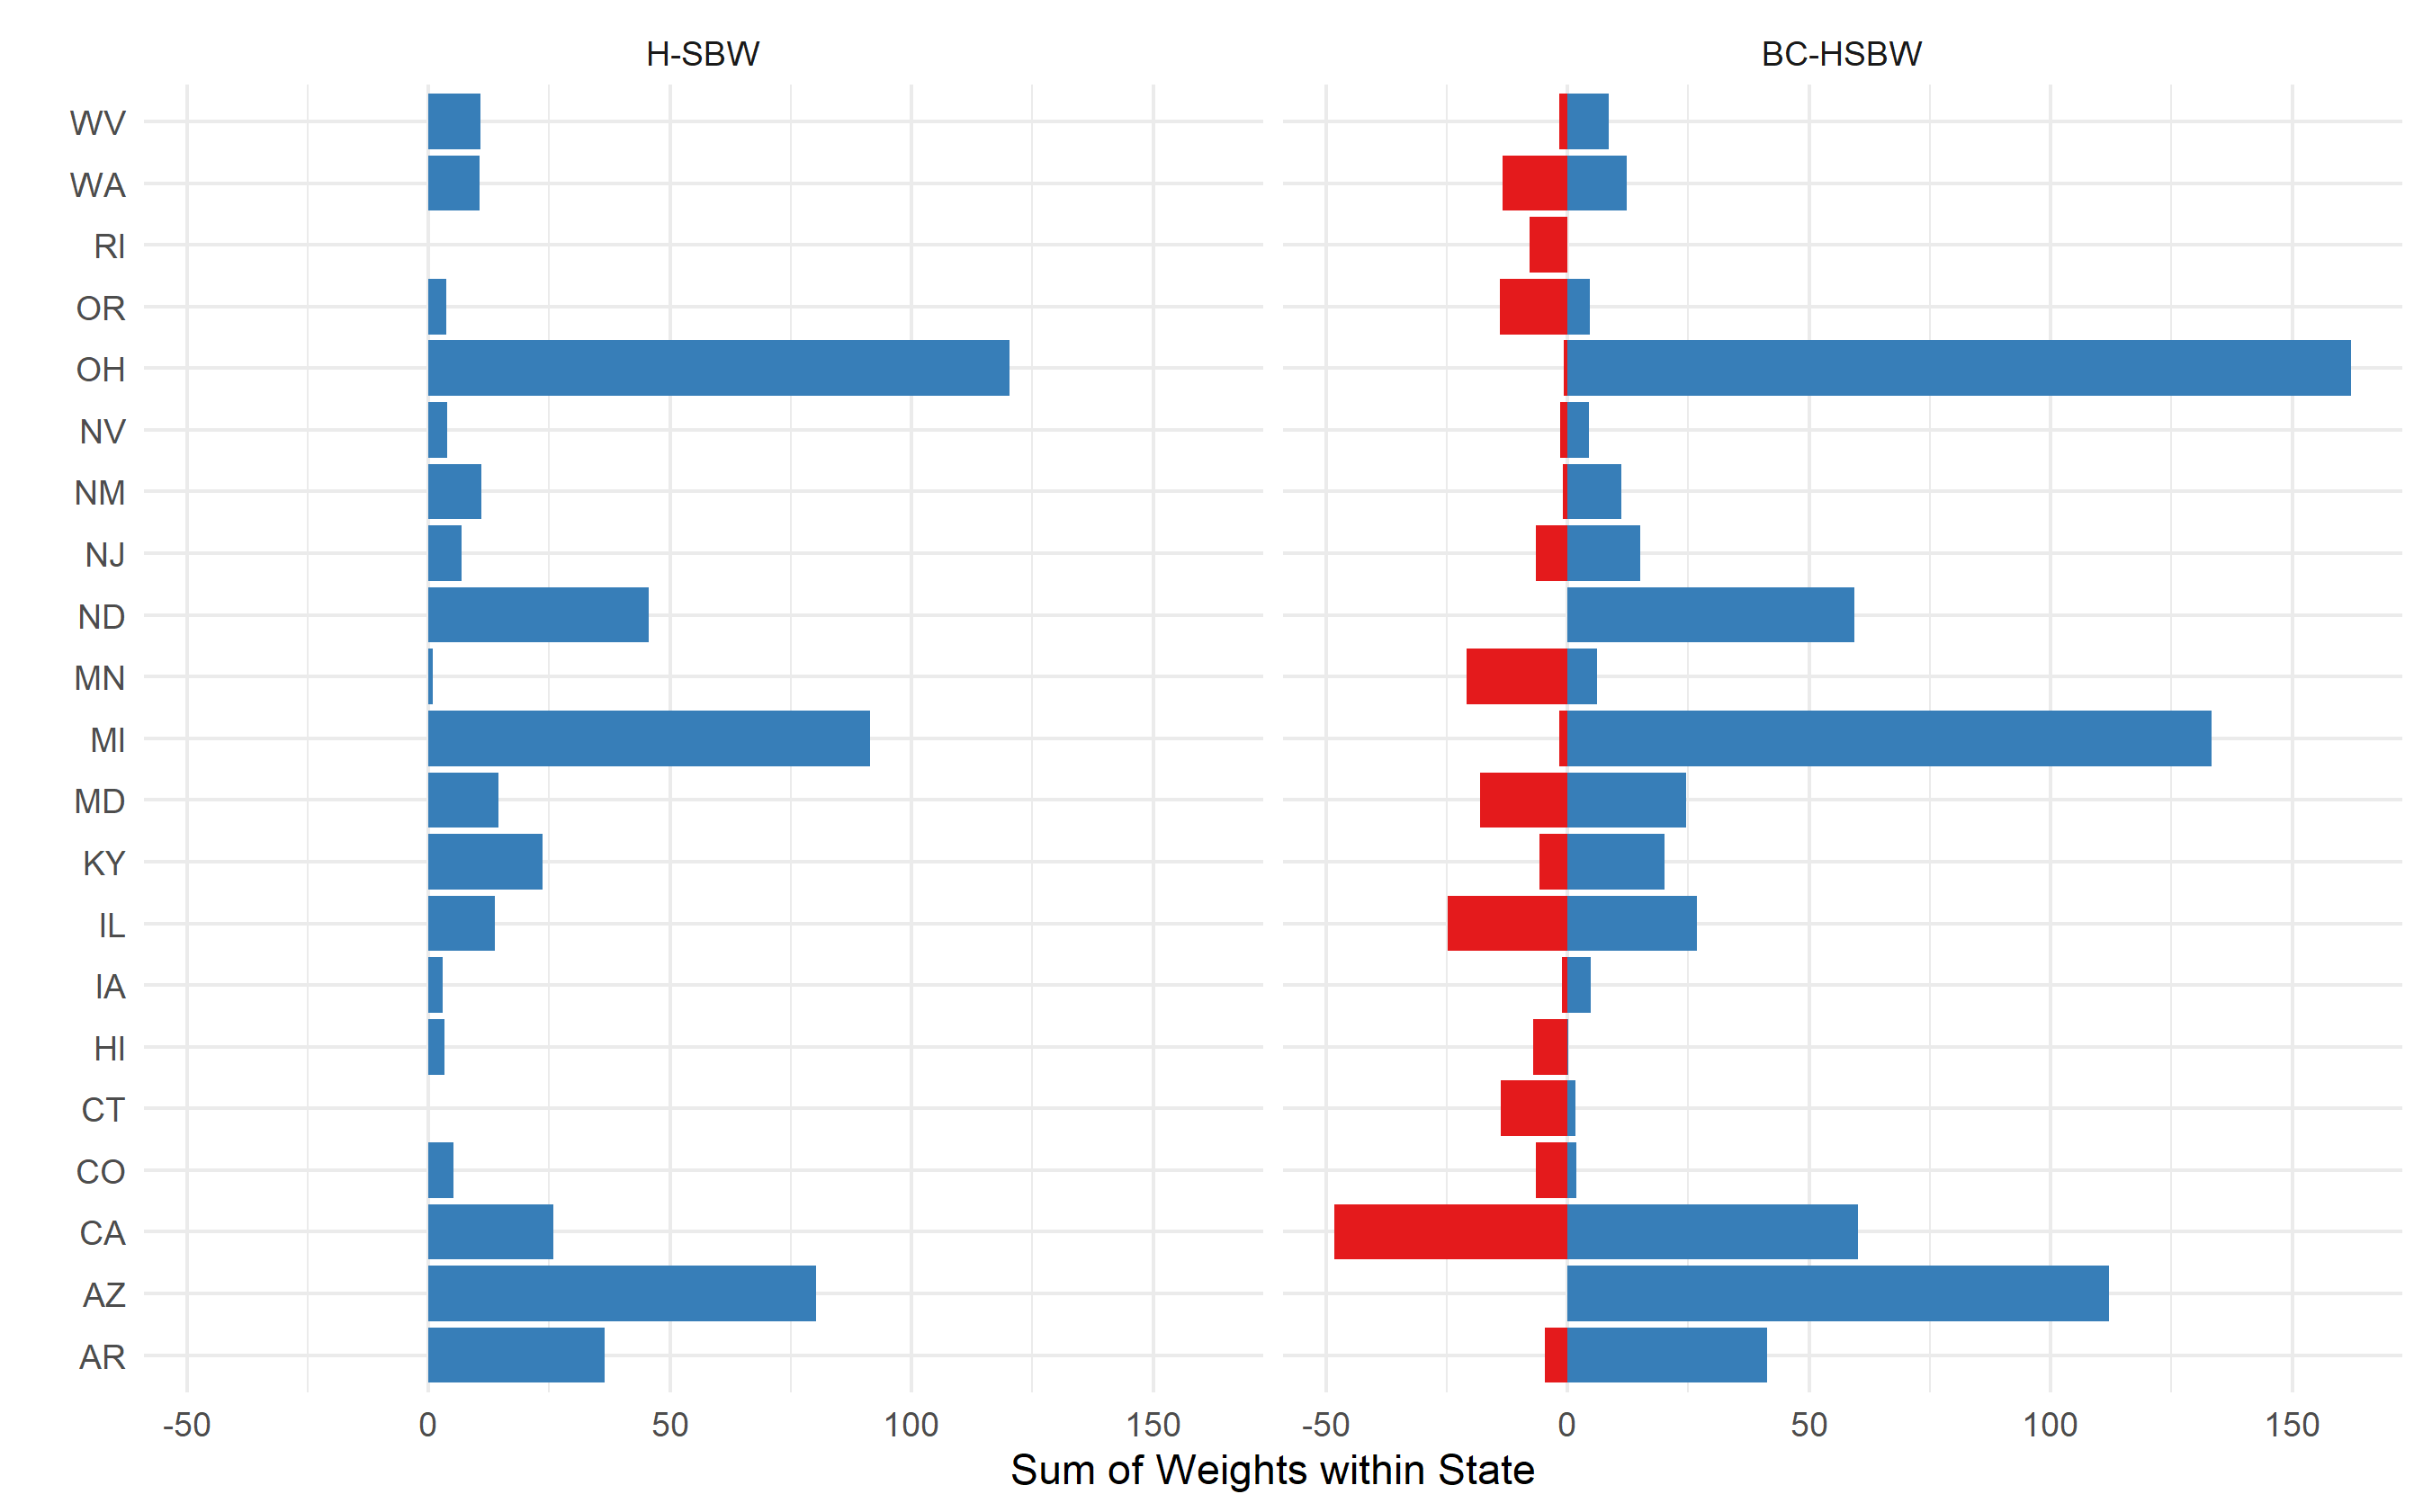
\includegraphics[scale=0.6]{01_Plots/weights-by-state-hsbw-c1.png}
\end{center}
\end{figure}

\subsection{Primary Results}

Using H-SBW we calculate an estimated effect of -1.94 (-3.56, -0.32). In other words, we estimate that had states that did not expand Medicaid in 2014 done so, they would have seen a 2 percentage point reduction in their uninsurance rates that year. While remaining imbalances are quite large, the bias-correction makes little substantive difference, yielding an estimate of -2.09 (-3.54, -0.63). These estimates differ somewhat from the estimates we find running the procedure on our unadjusted covariate estimates: here H-SBW gives an estimated effect of -2.21 (-3.22, -1.20), and the bias corrected estimator yields -2.44 (-3.40, -1.48). Using the adjusted covariate set appears to both move our estimate closer in absolute magnitude towards zero and decreases the width of the estimated confidence intervals. Figure~\ref{fig:estimators} displays the point estimates from these weighting estimators, as well as estimators using SBW, on the adjusted and unadjusted datasets. Additional results are available in Appendix E.

\begin{figure}
\begin{center}
    \caption{Point estimates}
    \label{fig:estimators}
    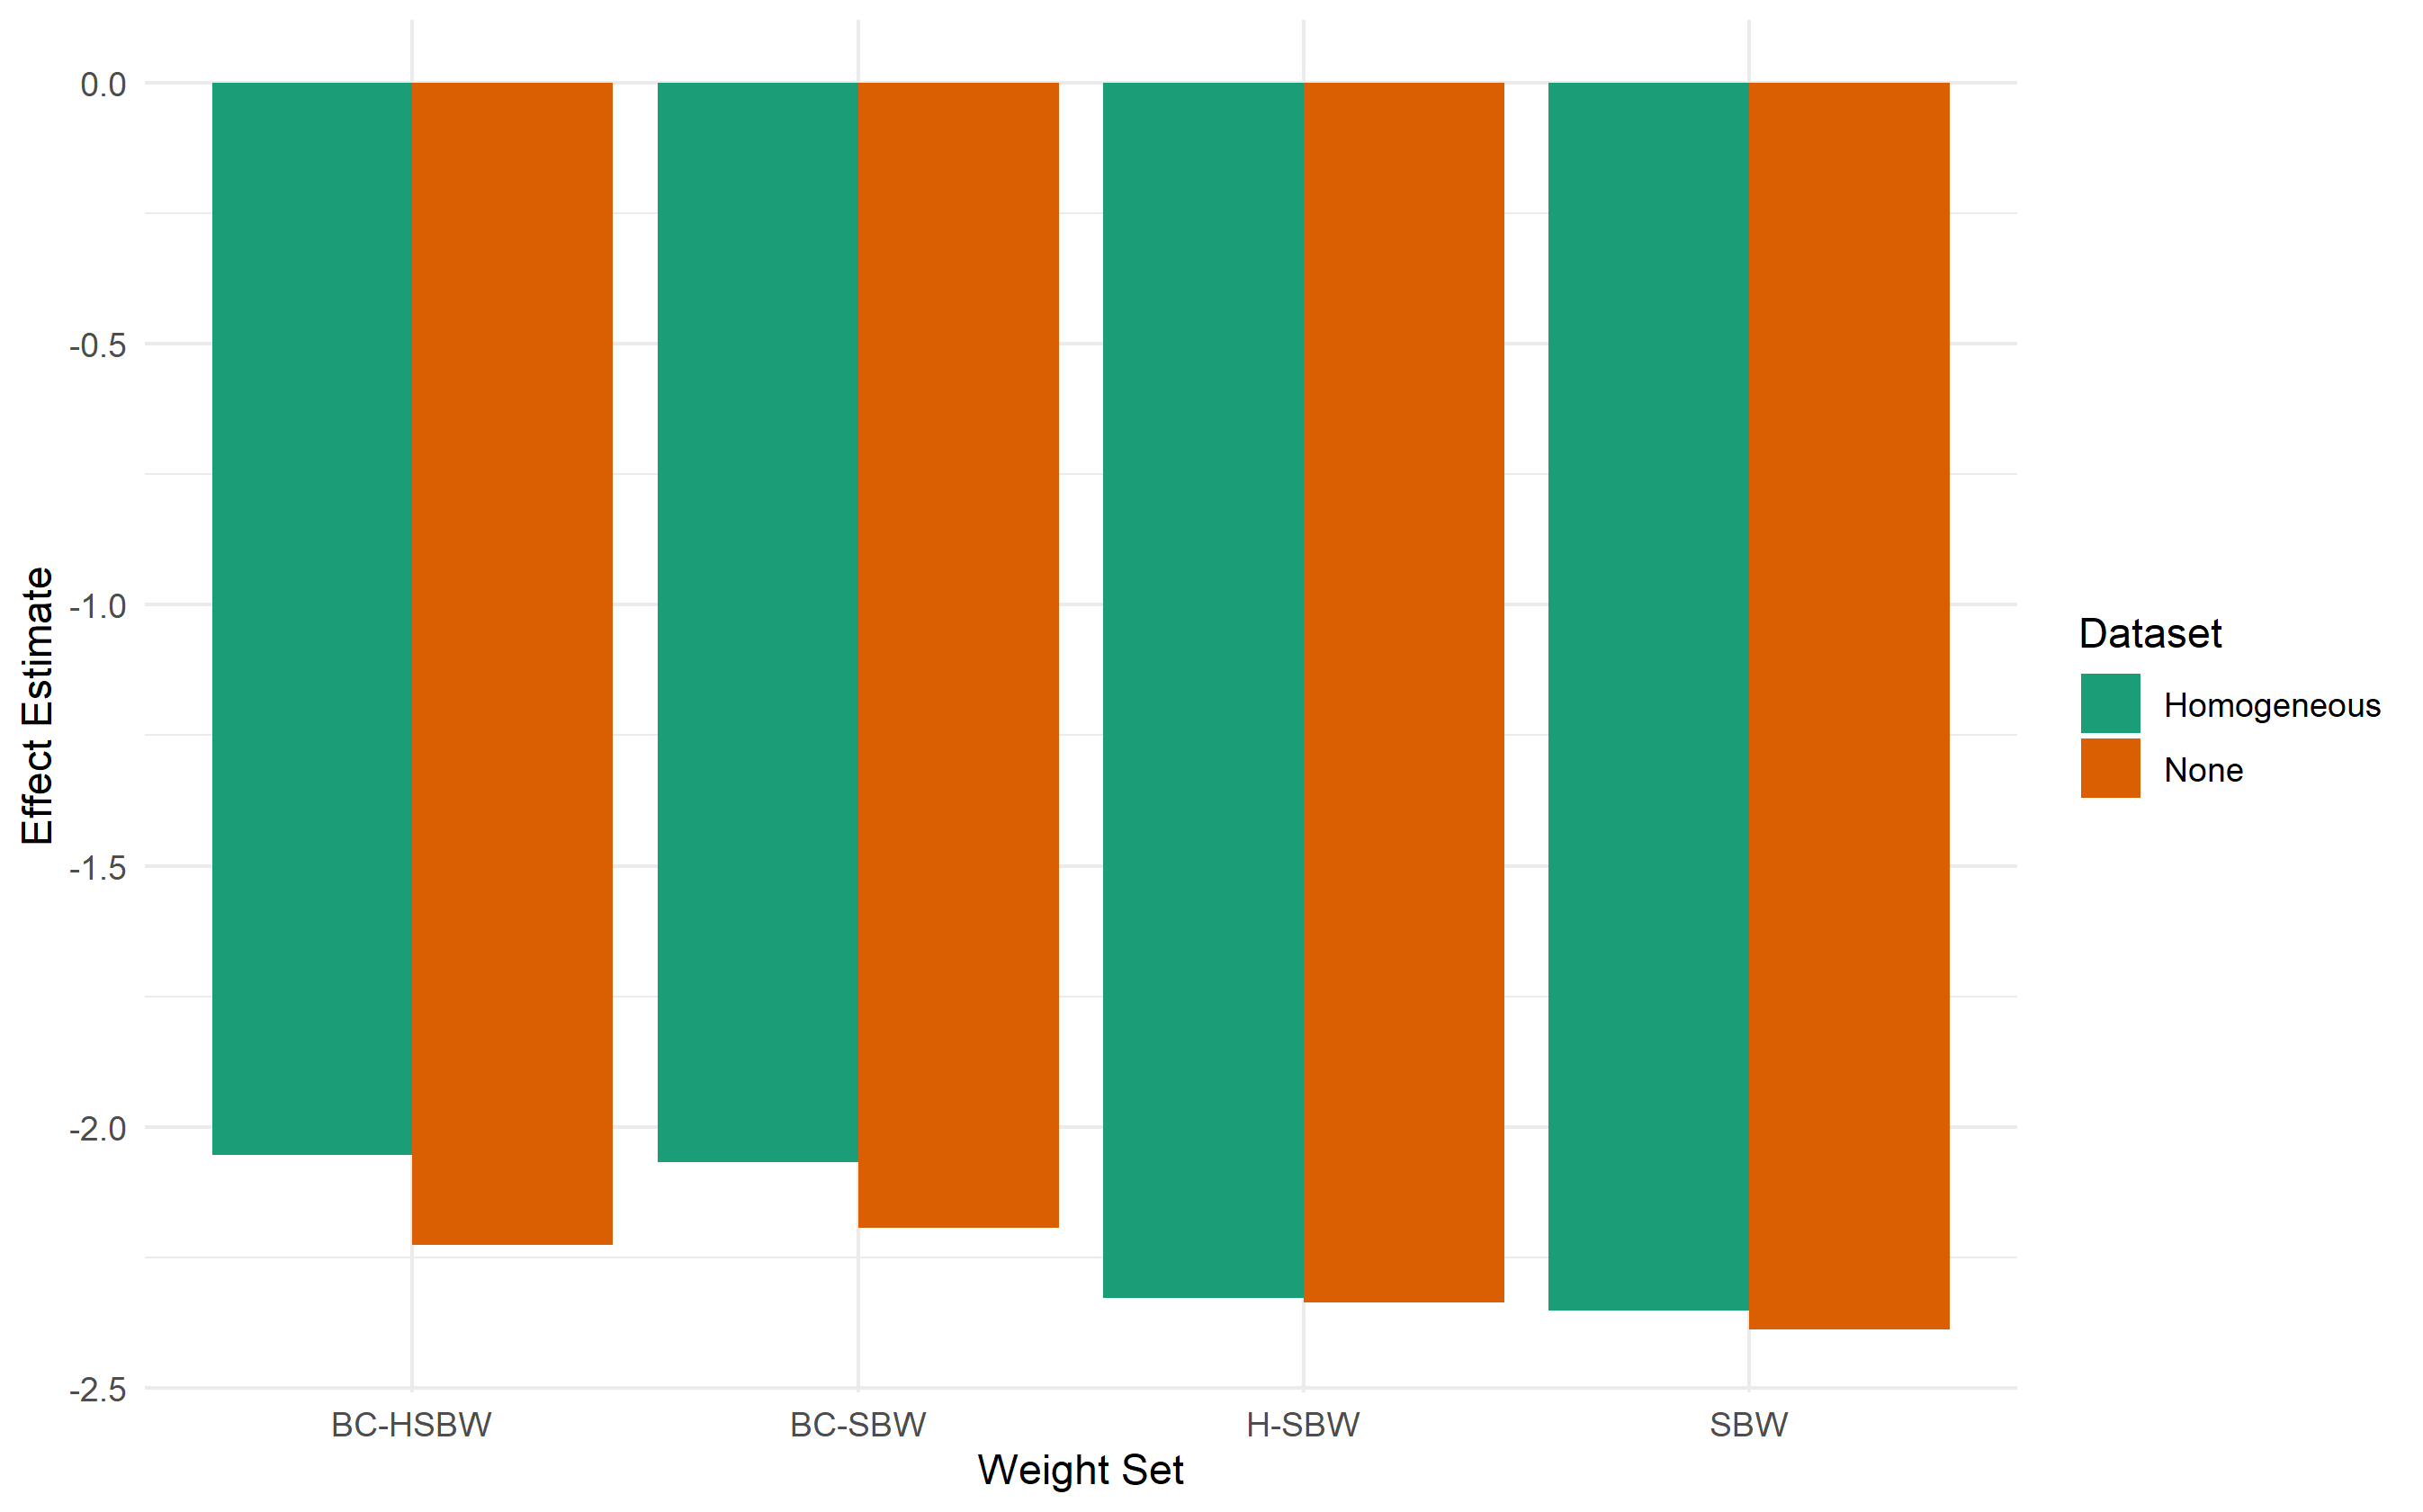
\includegraphics[scale=0.6]{01_Plots/point-estimates-c1.png}
\end{center}
\end{figure}

We examine the robustness of our point estimates to the removal of individual states (note that these are the point estimates used to calculate our confidence intervals). Figure~\ref{fig:loostateplot} shows how the point estimates change for both the adjusted (``sigma\_uu\_i\_modeled'') and unadjusted (``sigma\_zero'') datasets. We see similar results in either case: removing Ohio and Arkansas tends to increase the absolute magnitude of the point estimates. By contrast, removing California decreases the absolute magnitude of the estimators, particularly for estimators that are not bias-corrected. The results are quite similar when using different covariate adjustments and when recalculating the entire procedure (additional results are available in Appendix E, Table~\ref{tab:loostatec1}). 

\begin{figure}
\begin{center}
    \caption{Estimator sensitivity to states}
    \label{fig:loostateplot}
    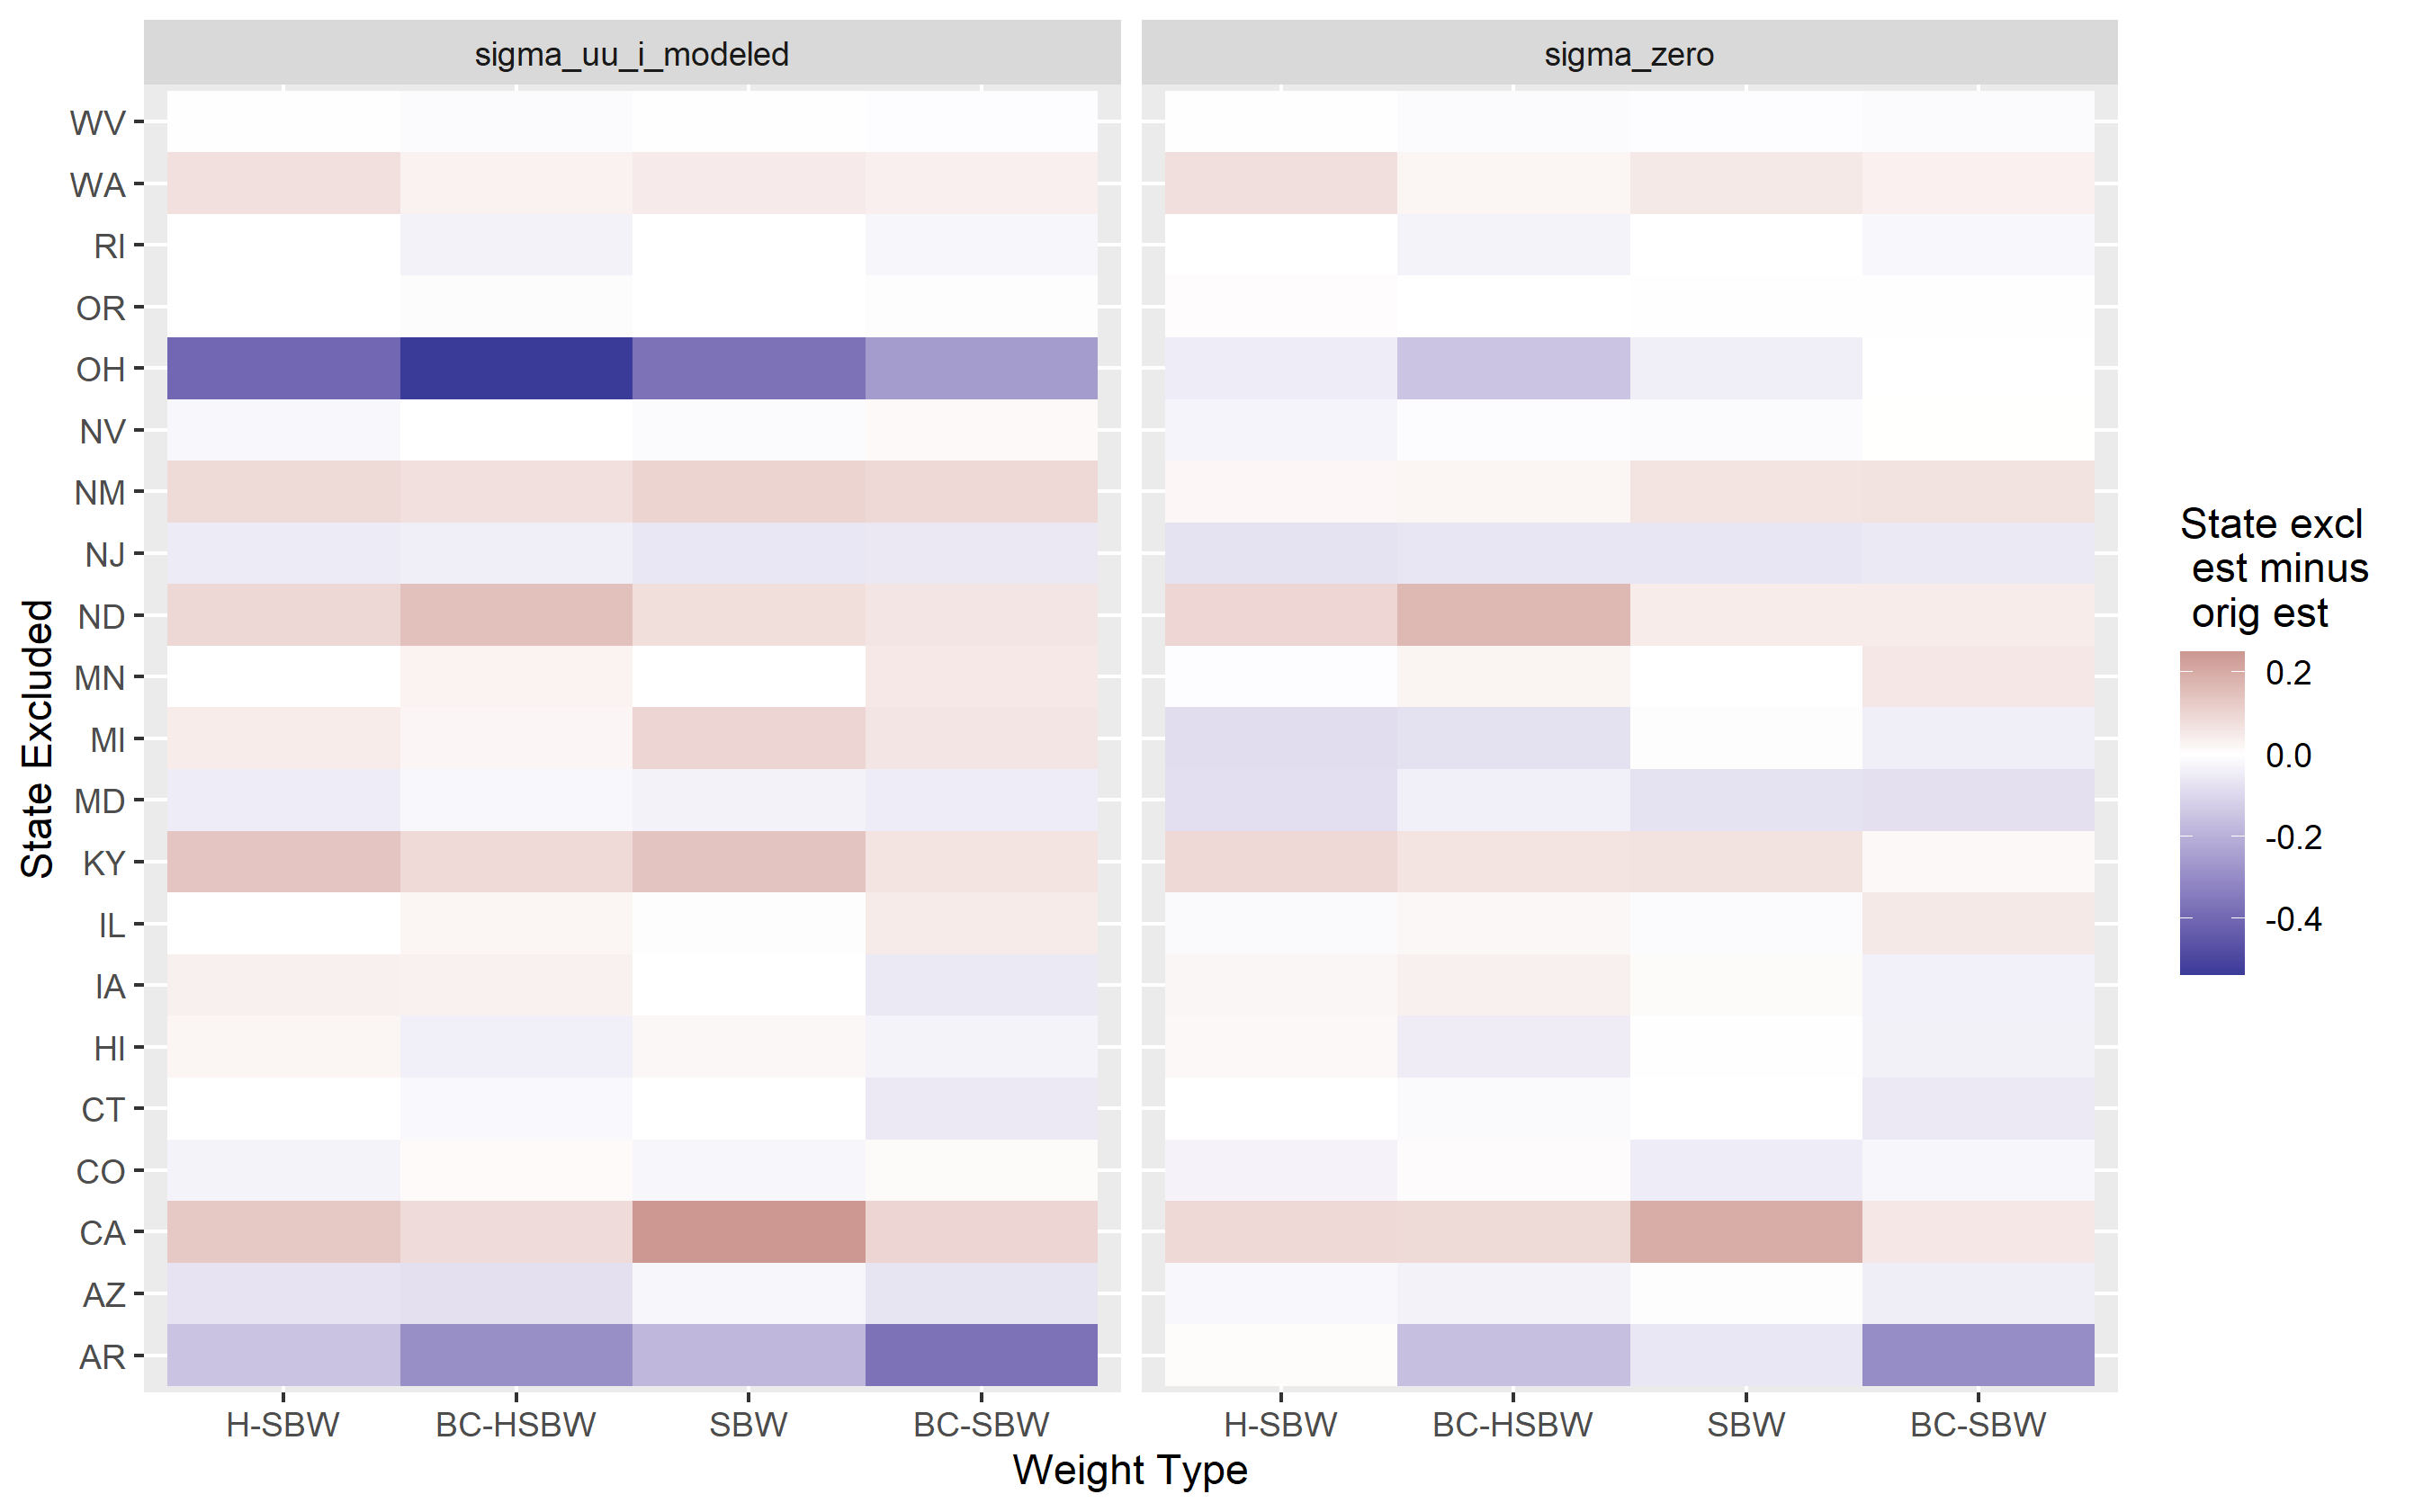
\includegraphics[scale=0.6]{01_Plots/loostate-sensitivityc1-state-uu-i.png}
\end{center}
\end{figure}

We now consider our second research question: whether Republican governance might be an effect modifier for the treatment effect. Let $\hat{\Delta}$ be the difference in estimators when removing the Republican governance indicators compared to the original estimate.\footnote{We also consider four other covariate sets and present these results in Appendix E, Table~\ref{tab:ptests}. None of these results are especially surprising, though we do see that controlling for pre-treatment outcomes and unemployment rates matters substantially for our point estimates.} For the H-SBW estimator we calculate $\hat{\Delta}$ equal to -0.62 (-2.05, 0.81) for BC-HSBW and -0.51 (-1.74, 0.71). We see similar differentials on our unadjusted dataset (-0.64 (-1.62, 0.34) and -0.49 (-1.33, 0.34), respectively). These results are consistent with our hypothesis that Republican governance drives heterogeneity in the effect of Medicaid expansion. While our confidence intervals include zero, we find that these differences are negative for all estimators we consider when removing each state (conditional on the covariate adjustment). That is, the sign of the differences in the contrasts remains negative for every specification that we run.\footnote{When we re-run the entire adjustment procedure when removing each state, we find that removing California results in a positive contrast between these estimates for BC-HSBW and BC-SBW and Illinois for BC-SBW for our adjusted dataset. However, this result only occurs with weights that extrapolate beyond the support of the data calculated on a covariate-adjusted dataset. We find that the covariate adjustments can lead to quite extreme imputed values for certain CPUMAs, particularly when we reduce the amount of data used to calculate the adjustment, a limitation of using a linear approximation to impute covariates that can only fall within a certain range. This problem compounds when allowing the weights to extrapolate because they are far more likely to use these bad estimates. Additional comments on these extreme values are available in Appendix C.} Overall we view this as suggestive (though not definitive) evidence consistent with our research hypothesis.

Appendix E Figure~\ref{fig:rdiffc1state} and Figure~\ref{fig:rdiffc1proc} display all estimates $\hat{\Delta}$ with each state removed, both conditional on the covariate adjustment and recalculating the covariate adjustment, respectively. Additional results for different estimators are available in Appendix E, Table~\ref{tab:deltac1}.

\subsection{Sensitivity Analyses} \label{sssec:sensitivity}

We examine the sensitivity of our analysis to violations of two key causal assumptions: (1) no anticipatory treatment effects, and (2) positivity violations. To the first point, several states had partial limited expansions prior to 2014. Following \cite{frean2017premium}, these states are California, Connecticut, Minnesota, New Jersey, and Washington. We rerun our analyses excluding CPUMAs from all five of these states. It is unclear how removing these states might affect our estimates: on the one hand, states that expanded early might have a smaller treatment effect after 2014 because they already enrolled newly eligible individuals. On the other hand, if these states were also more motivated to enroll people in Medicaid, they might have larger post-expansion coverage gains. Figure~\ref{fig:weightsbystatec2} displays the H-SBW weights summed by state alongside BC-HSBW. We again see that the BC-HSBW estimator extrapolates heavily to reduce the imbalances. A complete balance table is available in Appendix D, Table~\ref{tab:baltab1} and Table~\ref{tab:baltab2}.

\begin{figure}
\begin{center}
    \caption{Total weights summed by state, early expansion removed}
    \label{fig:weightsbystatec2}
    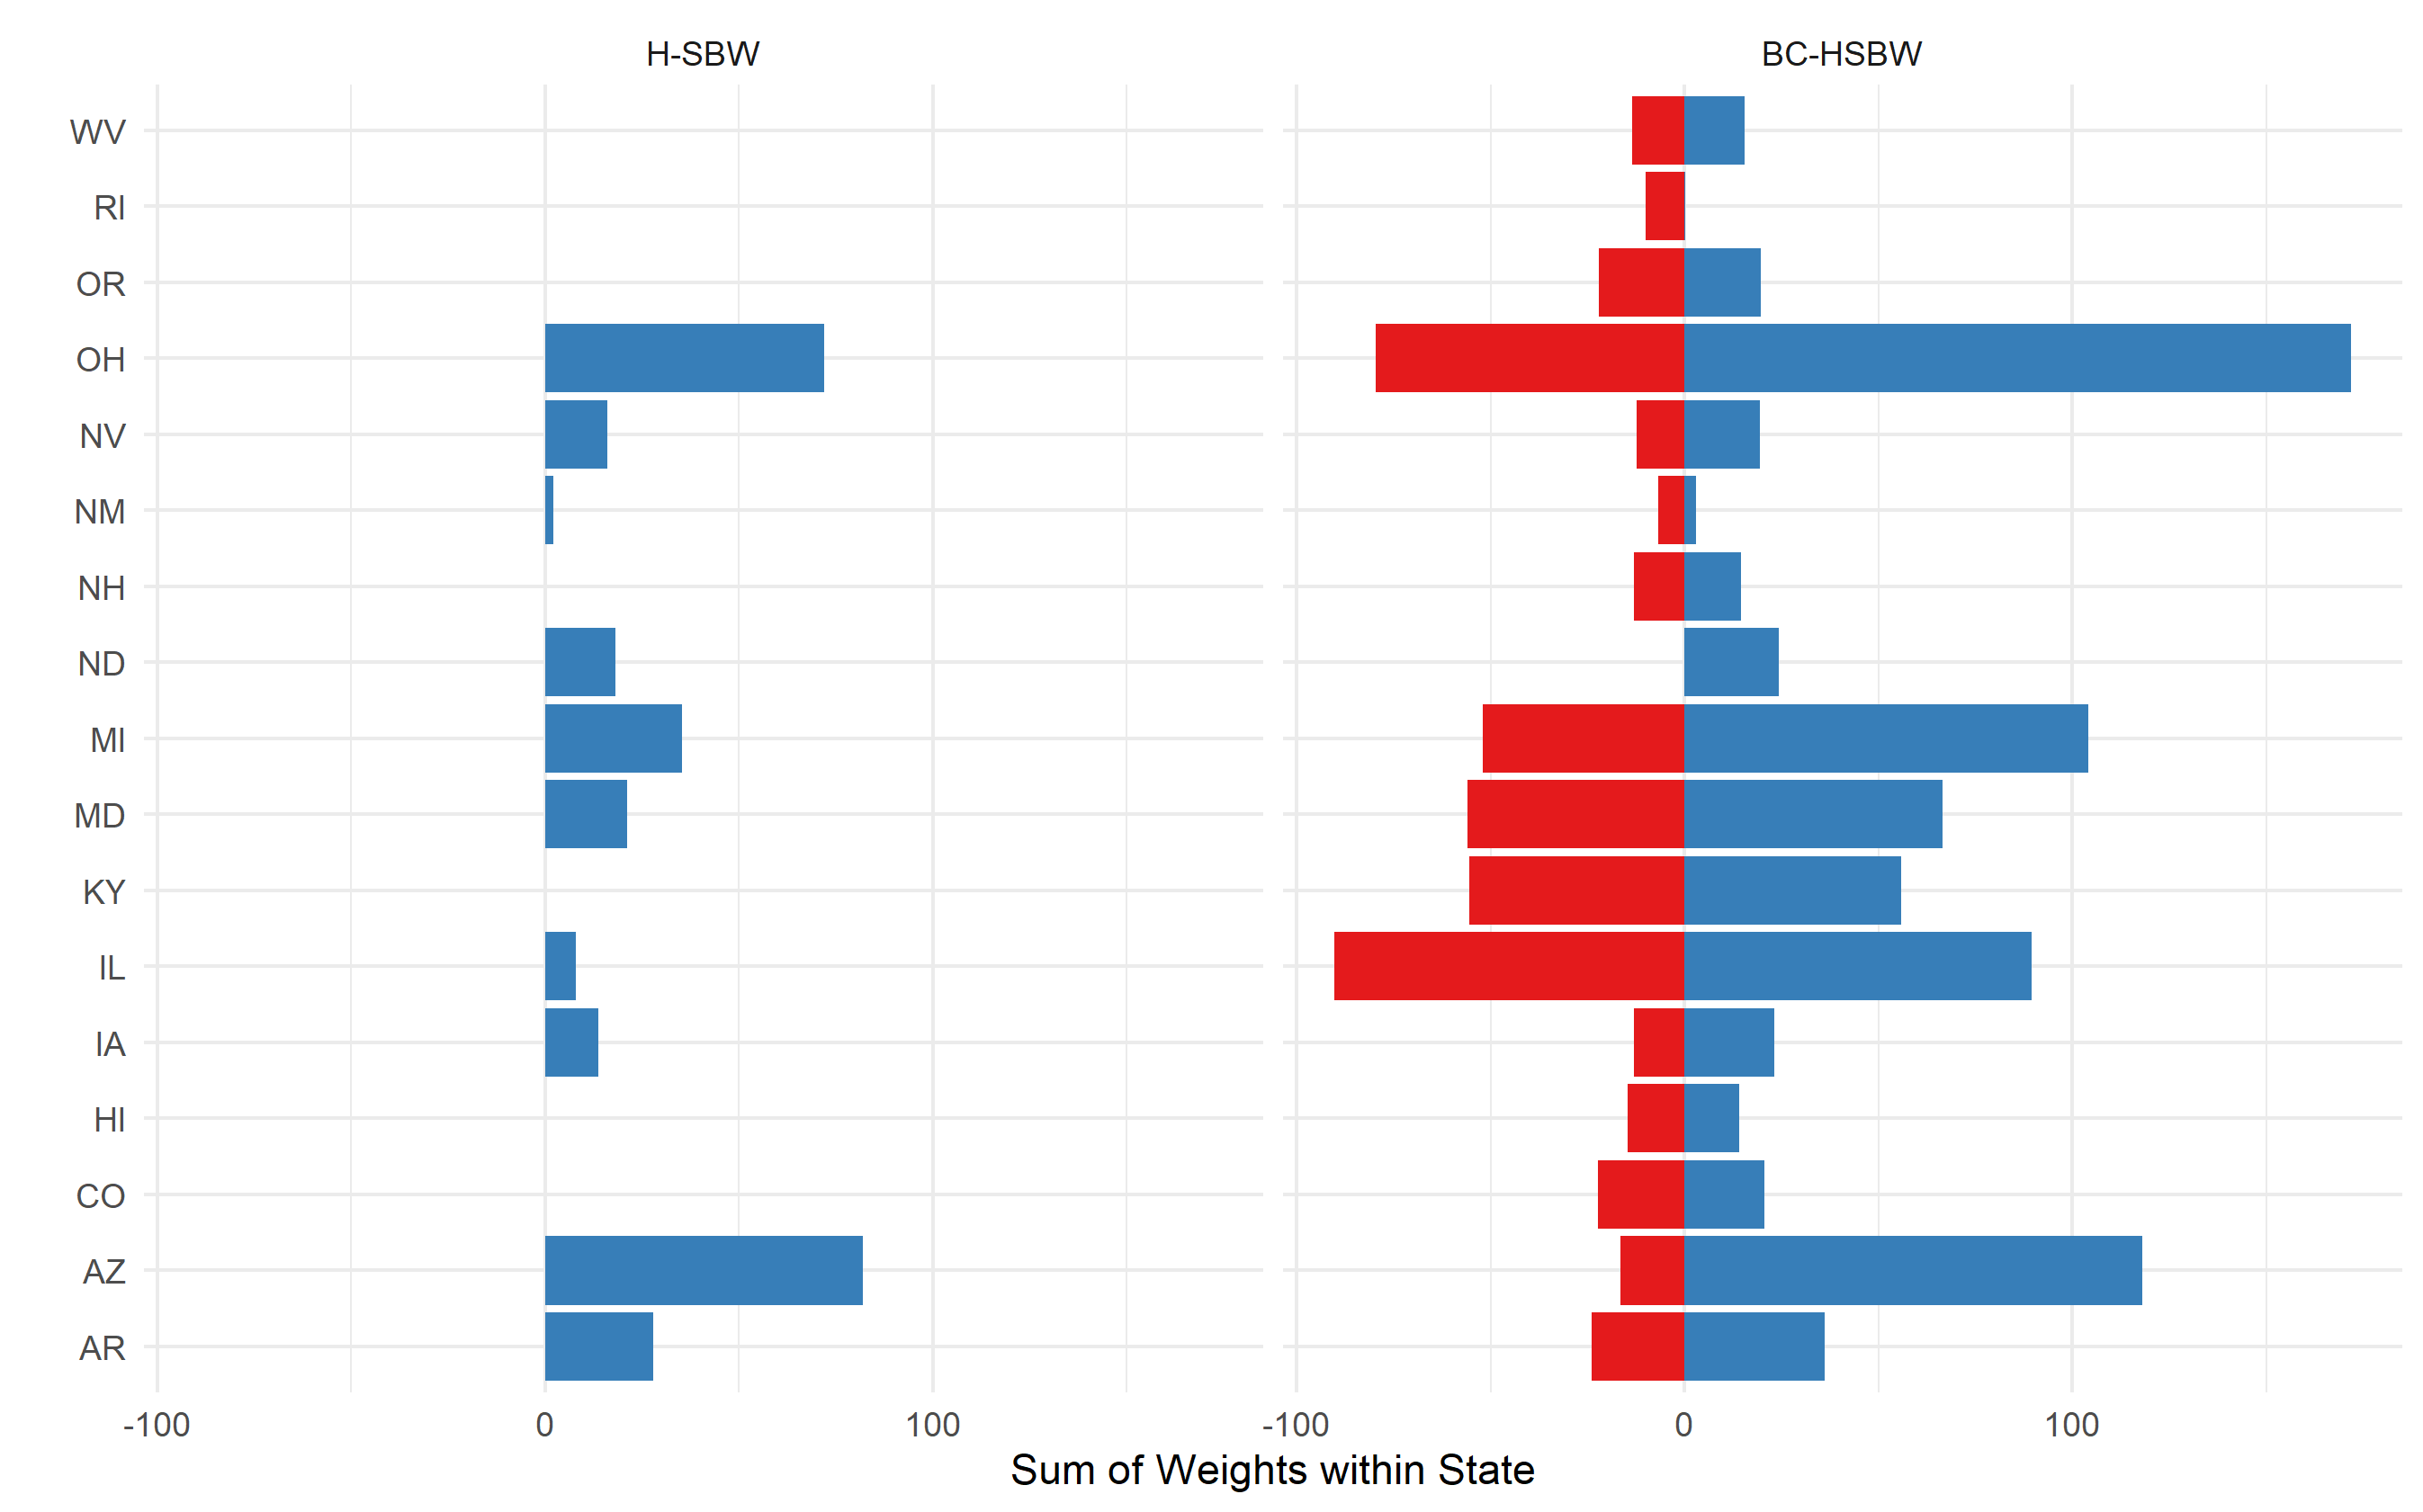
\includegraphics[scale=0.6]{01_Plots/weights-by-state-hsbw-c2.png}
\end{center}
\end{figure}

On this dataset we estimate an effect of -1.48 (-2.91, -0.06) using H-SBW weights; BC-HSBW yields an estimate of -2.06 (-3.72, -0.41). Here we see that the bias correction makes a larger substantive difference to the point estimate; however, it is not substantively different from the original point estimate with all states included. Overall we view this as evidence that our primary point estimates are fairly robust to the exclusion of these states, though perhaps the true effect is smaller in absolute magnitude. Table~\ref{tab:confintmainc2} and Table~\ref{tab:secondaryptests} in Appendix E display additional results. 

We also find that our estimates $\hat{\Delta}$ increase in absolute magnitude. Specifically, we find -1.15 (-2.53, 0.24) percentage point decrease for the H-SBW estimator when excluding the Republican governance indicators and a -0.74 (-2.40, 0.91) increase for BC-HSBW. Figure~\ref{fig:repub} displays these differences in the contrasts against those from our primary dataset. On our unadjusted dataset we estimate contrasts of -1.04 (-2.01, -0.07) and -0.61 (-1.75, 0.52). While these confidence intervals mostly contain zero, we again find that each individual difference between the leave-one-out-states estimated contrasts is less than zero (conditional on the covariate adjustment). These results again are consistent with our hypothesis that factors associated with Republican governance reduce the effect size of Medicaid expansion. Additional results are available in Appendix E, Table~\ref{tab:deltac2}. 

\begin{figure}
\begin{center}
    \caption{Removing Republican Governance Indicators}
    \label{fig:repub}
    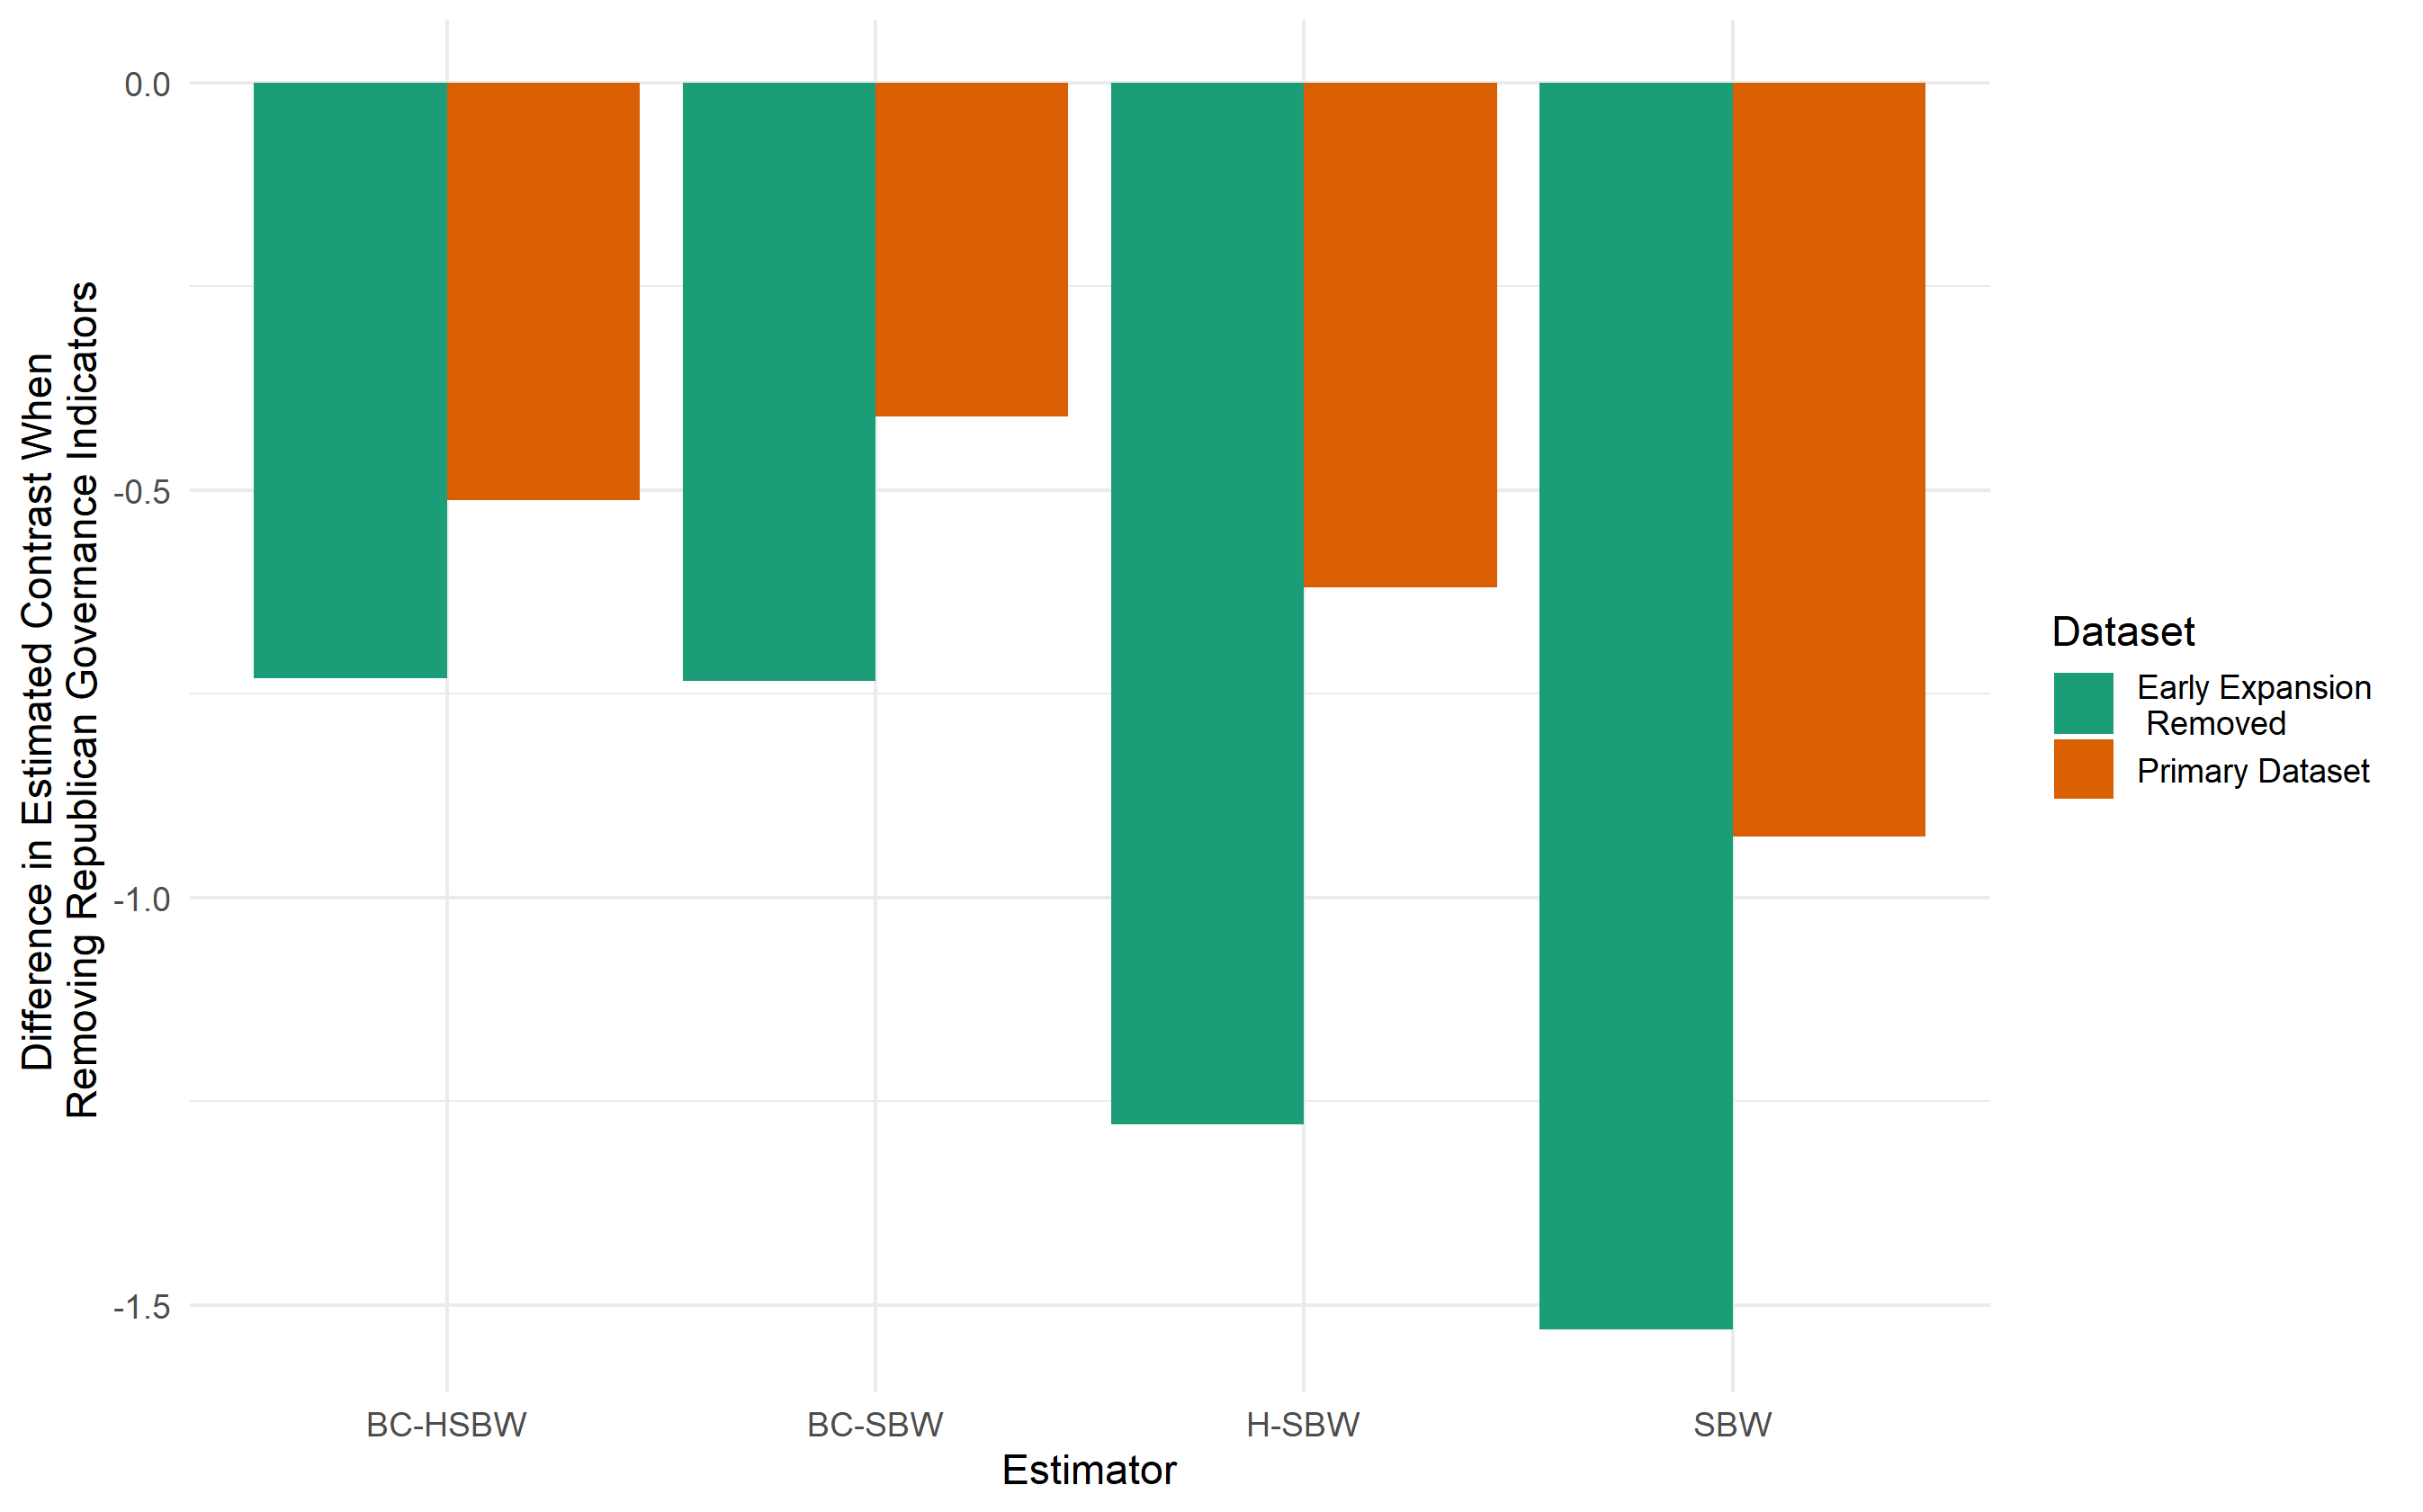
\includegraphics[scale=0.6]{01_Plots/repub-diff-c1c2.png}
\end{center}
\end{figure}

We conclude by considering an alternative method to account for positivity violations. To this point we have relied on either (1) retaining a potentially biased estimate from weights that do not provide exact balance, or (2) producing a more model-dependent estimate that relies on extrapolation. Overall we found that the results did not change substantially either way. Here we consider a third option: changing our target estimand. In particular, we consider the overlap average treatment effect (OATE), proposed by \cite{li2018balancing}. This is the treatment effect on the subset of the entire dataset where we have overlap. It is a data-dependent treatment effect, and is not the same as the treatment effect on the untreated; however, we believe that this effect will be more similar to the ETC than the ETT, particularly because there were no Democratic controlled states that did not expand Medicaid. Indeed, after generating overlap weights on our primary dataset we find that across all covariates, the mean average absolute distance from the overlap region to the untreated region is 2.92 and to the treated region is 7.80.\footnote{The distance is between the overlap region calculated as an unweighted mean on the adjusted datasets.} Figure~\ref{fig:oatearea} displays the distance between covariates with greater than one percentage point distance from the overlap region to either the control or treated region. We see that the overlap region is substantially more Republican than the treated region, as expected. This region is also less Hispanic, more white, less rural, and more educated than either the expansion or non-expansion region. Table~\ref{tab:oatedist1} and Table~\ref{tab:oatedist2} in Appendix D show additional statistics on the OATE region versus the treatment and control regions for all covariates.

\begin{figure}
\begin{center}
    \caption{Overlap area compared to treated, untreated regions}
    \label{fig:oateimbalance}
    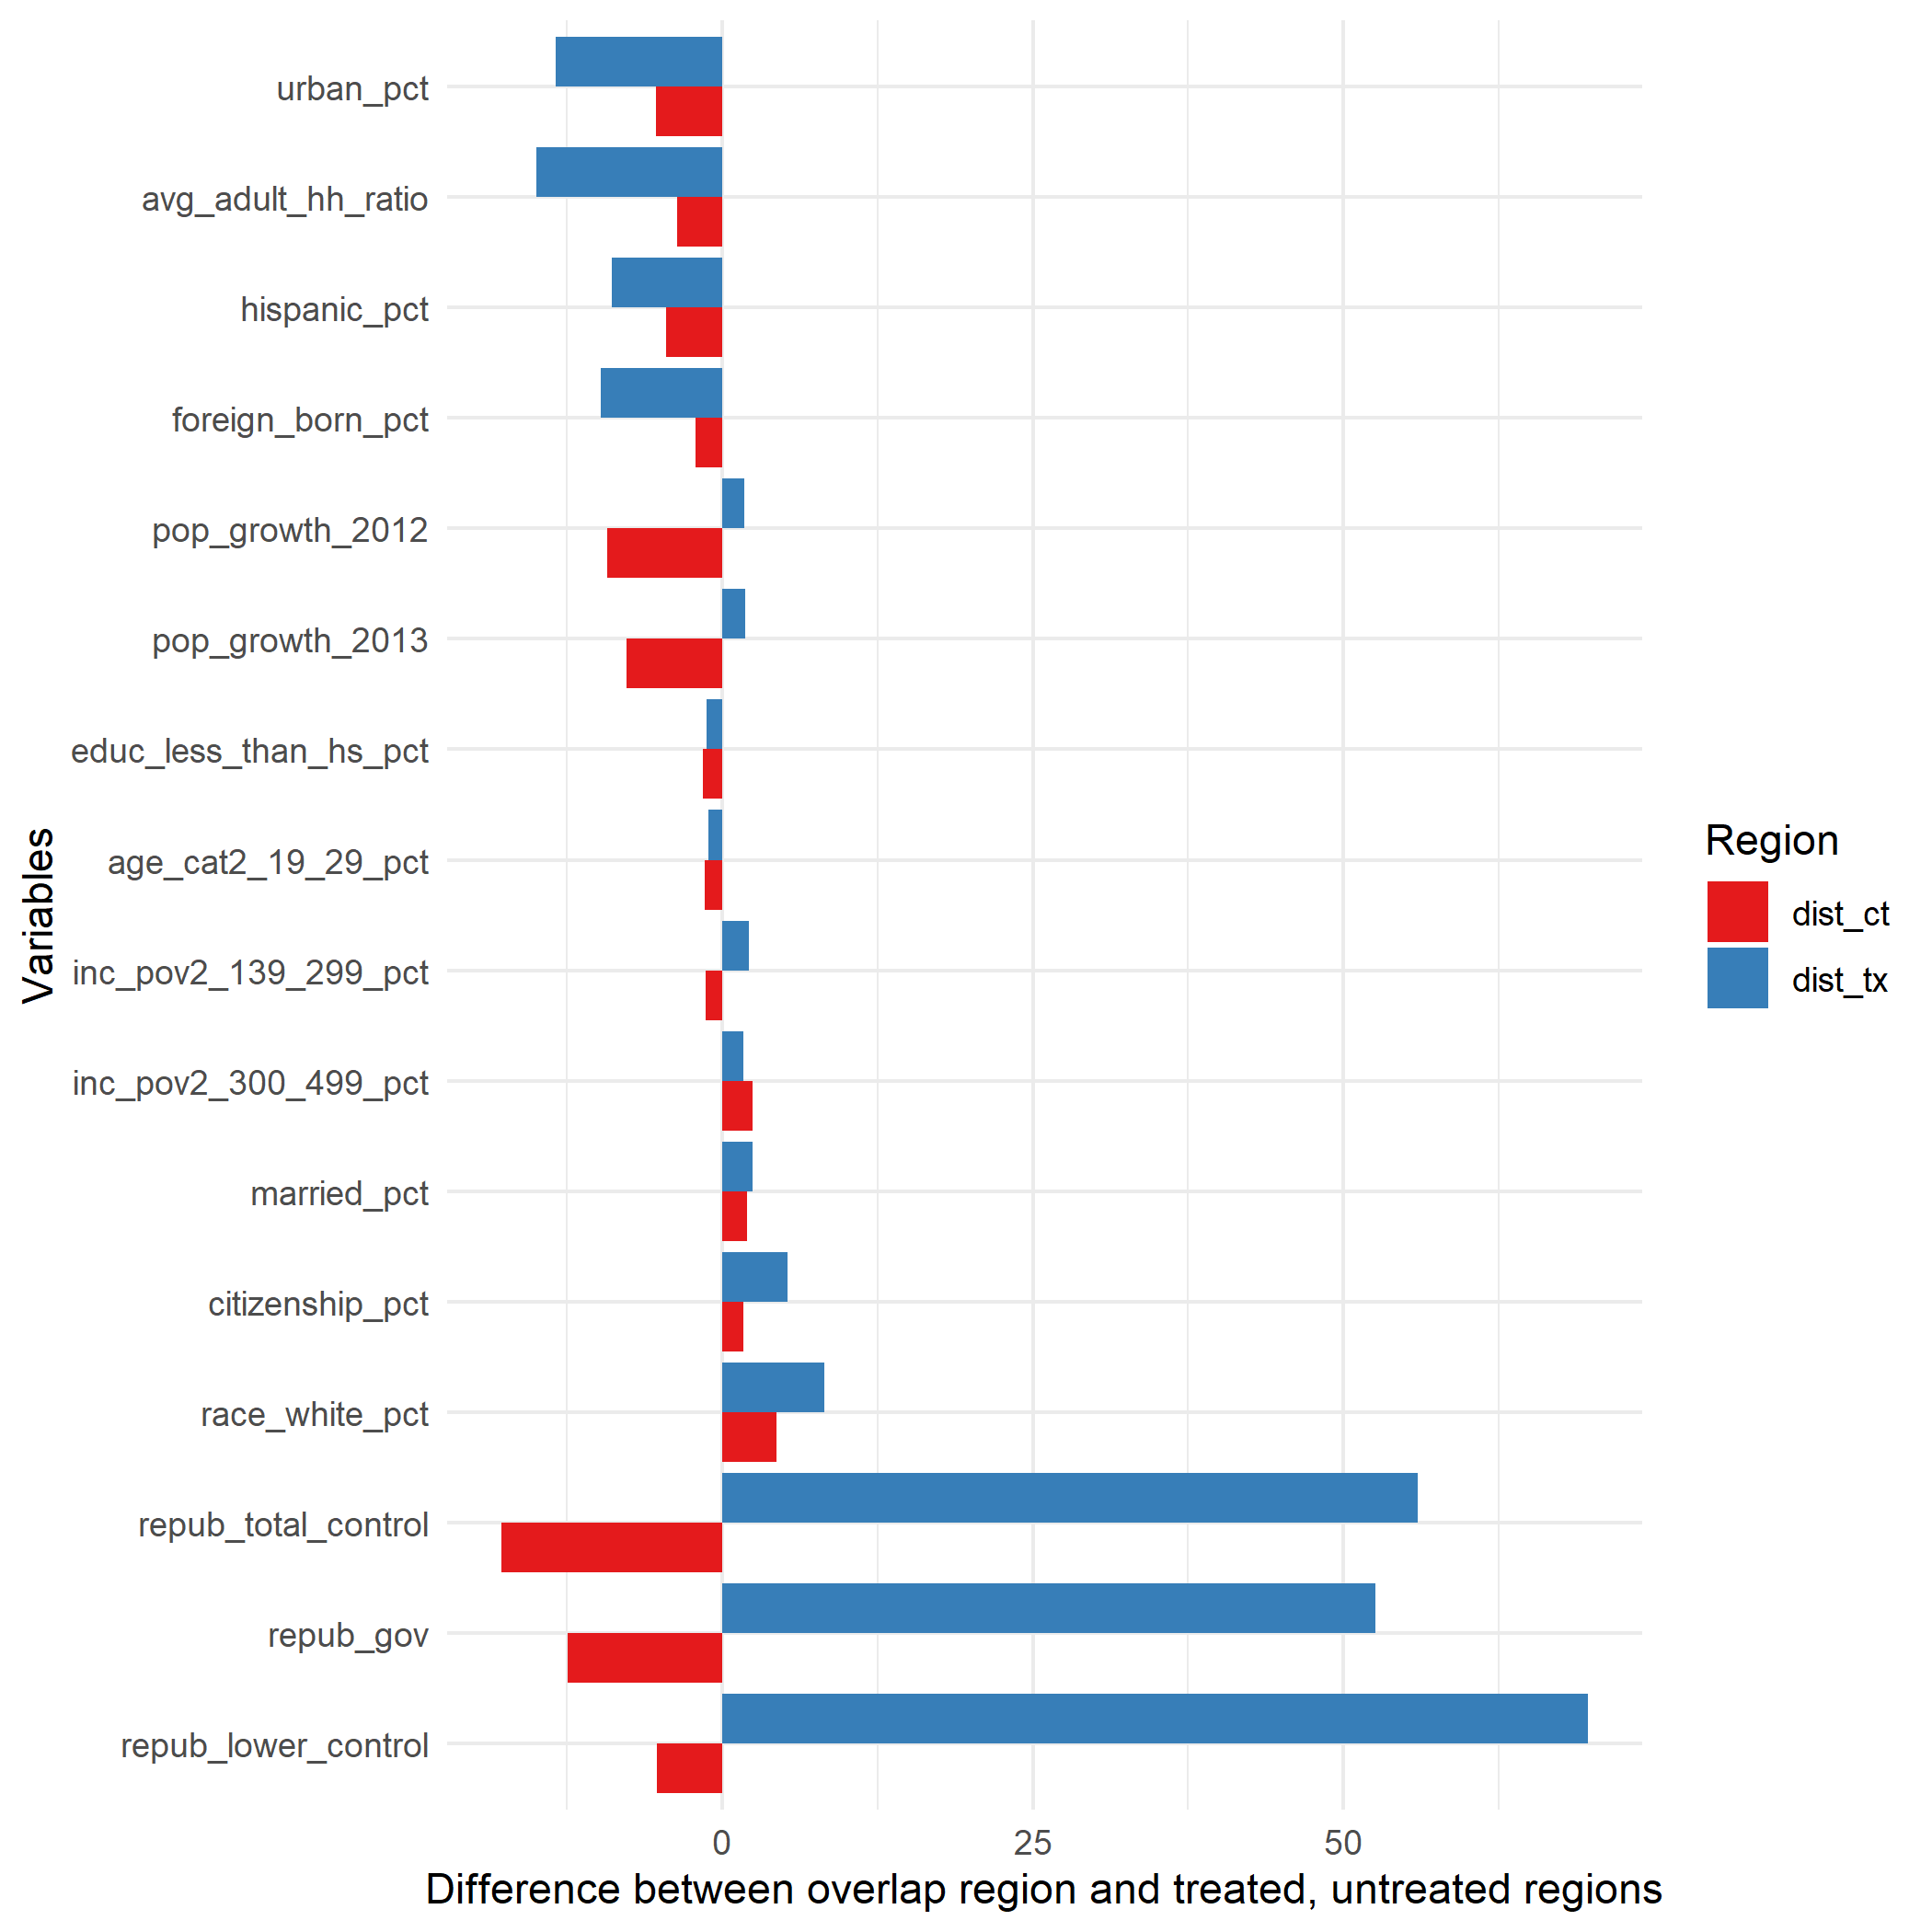
\includegraphics[scale=0.6]{01_Plots/oate-imbalances.png}
\end{center}
\end{figure}

Figure~\ref{fig:oateimbalance} displays the sum of the weights within each state by treatment group. Ohio, Michigan, and Arkansas, which all expanded Medicaid, are the most heavily weighted states (the weights are standardized to sum to 100). The weights are more evenly dispersed among the non-expansion regions, though Pennsylvania, Missouri, Wisconsin, and Florida are given the most weight. We note that this region is specific to the preferred covariate adjustment; the results are quite similar for the unadjusted and less preferred covariate adjustment and are available in Appendix D, Table ~\ref{tab:oatestateweights}.

\begin{figure}
\begin{center}
    \caption{Overlap weights by state}
    \label{oatearea}
    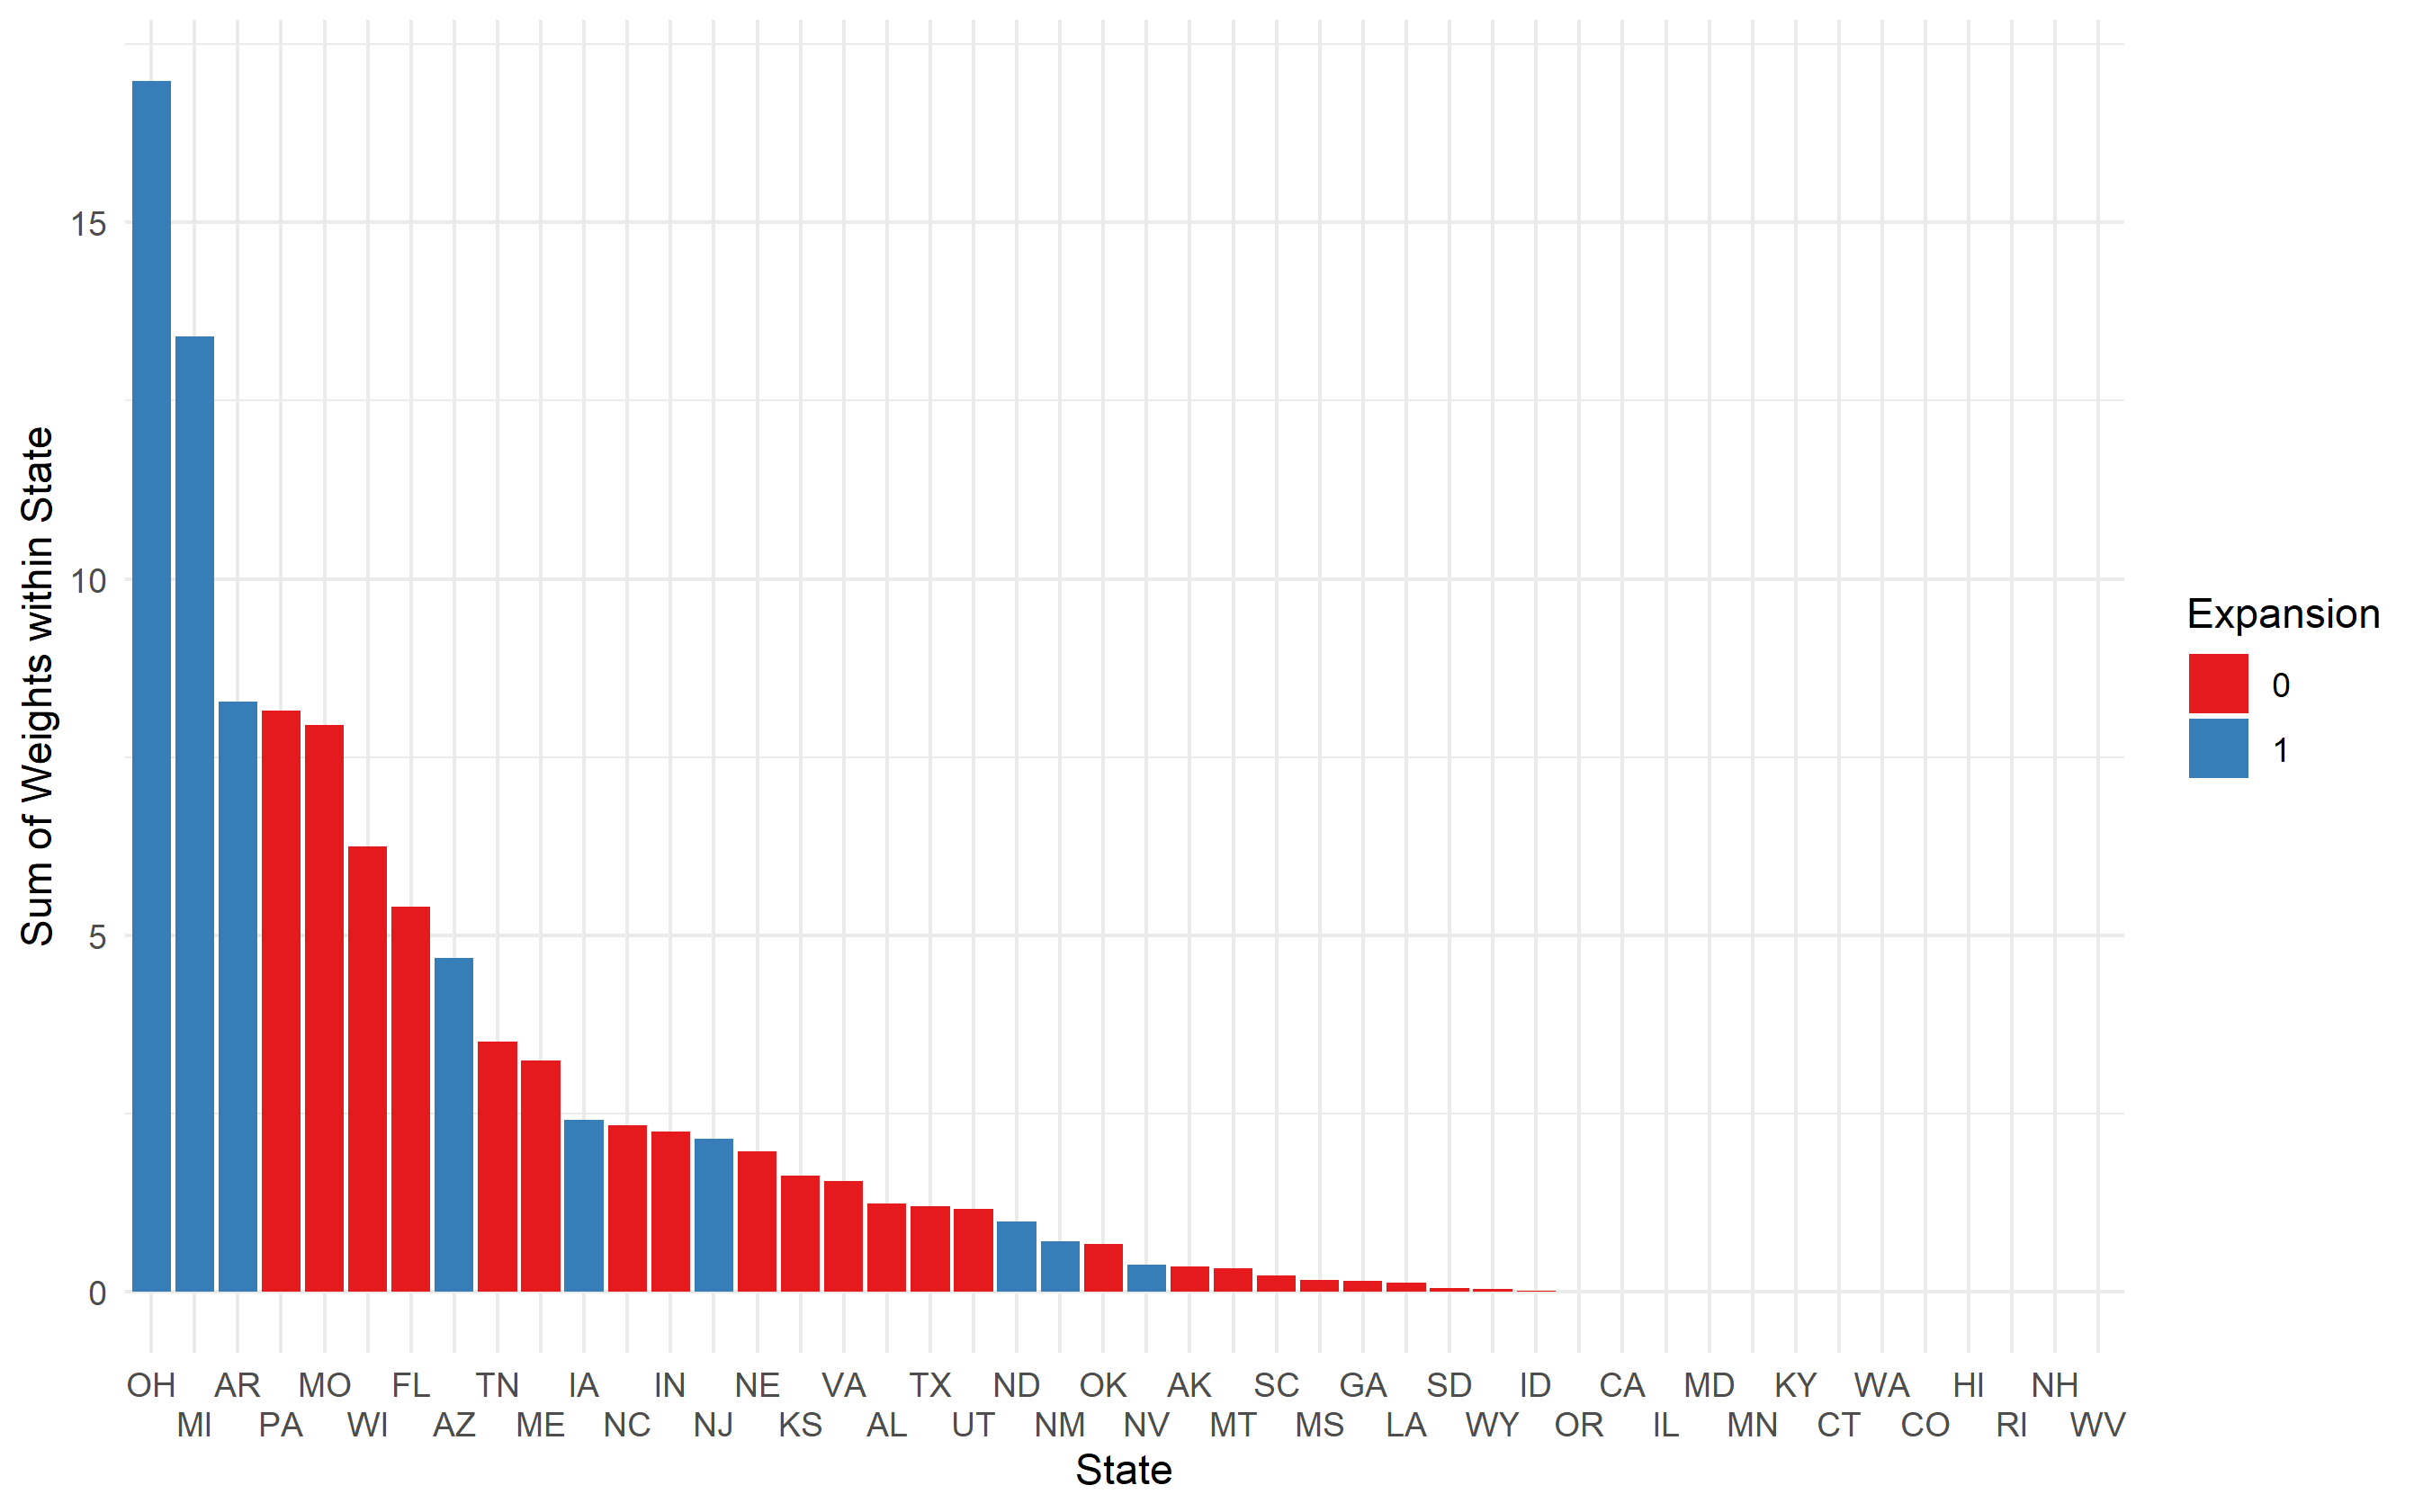
\includegraphics[scale=0.6]{01_Plots/oate-region-c1-a.png}
\end{center}
\end{figure}

We find similar results to our primary analysis: within the overlap region we estimate a treatment effect -1.64 (-2.40 -0.89) when including all treatment states in our primary analysis, and of -1.81 (-2.47, -1.15) when excluding the early expansion states. The results are quite similar when we use the unadjusted datasets: -1.80 (-2.49, -1.10) on the primary dataset and -1.95 (-2.65, -1.25) when excluding early expansion states. 

We again find a negative difference when comparing an estimate excluding the Republican governance indicators against our primary estimate: specifically, we find that the estimate decreases by -0.96 (-0.81, -1.10) percentage points on the primary dataset and by -0.62 (-0.78, -0.46) percentage points when removing early expansion states. \footnote{Unlike the ETC, this contrast is a function of the differences in the weighted covariates among both the treated and control regions.} Notice that both of these estimates were statistically significant; the confidence intervals increase only slightly when recomputing the entire adjustment when removing each state. Moreover, this negative difference in estimated contrasts holds for each excluded state, regardless of whether we conditioned on the adjustment or recalculated it. Additional results are available in Appendix E, Table~\ref{tab:oateconfint} and Table~\ref{tab:oatesensitive}. This result again supports our hypothesis that factors associated with Republican governance drive heterogeneity in the estimated treatment effects.

\section{Discussion}

We estimate that had states that did not expand Medicaid in 2014 instead expanded their programs, they would have seen a -2.00 (-3.59, -0.40) percentage point change in the adult uninsurance rate. Existing estimates place the ETT between -3 and -6 percentage points; these estimates vary depending on the targeted sub-population of interest, the data used, and the modeling approach (see, e.g., \cite{courtemanche2017early}, \cite{kaestner2017effects}, \cite{frean2017premium}). This ETC estimate is therefore closer to zero than these ETT estimates, supporting our original hypothesis that the treatment effect on non-expansion states would be smaller in absolute magnitude. Moreover, we also find suggestive evidence that factors associated with Republican governance may drive this differential. While much of this evidence was statistically insignificant, we believe that the consistency of this finding to many of our modeling specifications supports this hypothesis.

We also make several methodological contributions to the literature on balancing weights. First, we extend the synthetic controls literature to estimate the treatment effect on the controls. The key challenge is that we need to predict treatment response rather than the outcome absent treatment. Unlike when estimating the treatment effect on the treated, we cannot use pre-treatment outcomes to conduct variable selection, run placebo tests, or train our model in some other way. This is a fundamentally more difficult problem that requires greater modeling assumptions. Second, we extend the Stable Balancing Weights objective function for use with hierarchical data and covariates measured with error. We modify the criterion to more evenly disperse the weights across states, and the constraint set to balance on a linear approximation to the true covariate values using regression-calibration techniques (\cite{gleser1992importance}).

Our study's approach also has bearing on estimating and understanding the ETT using a differences-in-differences design when estimating the 2014 effects of Medicaid expansion. If we believe that Republican governance is associated with changes in trends over time, then we need to control for this factor. However, there is likely insufficient overlap to control for these factors without significantly extrapolating from the data. We see that the ETC requires less extrapolation than the ETT with respect to governance, and is therefore in some sense a more estimable quantity.\footnote{We note, however, that the standard parallel trends assumption used to identify the ETT is different to the no unmeasured confounding assumption we made here.} 

More generally, our results also suggest that we should not use estimates of the ETT to make inferences about the ETC. Because almost every outcome of interest is largely mediated through increasing the number of insured individuals, and because we have shown that there is likely treatment effect heterogeneity with respect to governance, projecting findings from an estimate of the ETT to the ETC would lead to inaccurate inferences. For example, \cite{miller2019medicaid} study the effect of Medicaid expansion on mortality. Using their estimate of the ETT they project that had all states expanded Medicaid, 15,600 deaths would have been avoided during their study's time-period. If we believe that the ETT were further away from zero than the ETC, we should expect that this projection is an overestimate. Directly estimating the ETC can therefore also help us better model interesting downstream effects mediated through increasing the number of insured individuals. 

Our results come with three major caveats: (1) we rely on strong parametric assumptions about the outcome model to estimate our causal effect; (2) our identification assumes no unmeasured confounding given the true covariates; (3) our estimated associations between Republican governance and our estimated treatment effect largely fall within our estimated margins of error. 

We conclude by discussing the policy implications of these findings. First, we note that a reduction of adult uninsurance rates by -2.00 percentage points represents approximately a 10 percent reduction in the uninsurance rate among non-expansion states. As observed previously, this estimated treatment effect is closer to zero than corresponding estimates of the ETT (see, e.g., \cite{courtemanche2017early}), and we may therefore expect that downstream effects that move away from zero monotonically with the number of uninsured are also closer to zero than estimates of the ETT. Second, we emphasize that the association we find between Republican governance and the estimated treatment effect is only an association: this finding does not imply, for example, that states with more conservative governments in general deliberately make Medicaid enrollment more difficult relative to Democratic states. As \cite{sommers2012understanding} notes, people may be less likely to enroll in Medicaid in conservative states due to social stigma and/or personal beliefs about the welfare state. Regardless of the true cause, to evaluate the policy implications of this finding, we compare this result against Congress's goal in implementing Medicaid expansion in the 2010 ACA, which was to increase health insurance coverage. Measured against this intent, better federal policies should encourage states to make Medicaid enrollment easier, for example, by making enrollment automatic. 

\section{Conclusion}

This is the first study to directly estimate the foregone coverage expansions of Medicaid expansion on states that did not expand Medicaid in 2014. We also contribute to the methodological literature on synthetic controls by clarifying the assumptions required to use longitudinal data to estimate the ETC rather than the ETT, and to the balancing weights literature more generally by considering the case where we have hierarchical data and covariates measured with error. We estimate that had states that did not expand Medicaid in 2014 done so, they would have seen a -2.00 (-3.59, -0.40) percentage point change in their uninsurance rate. This is substantially closer to zero than existing estimates of the ETT, which range between -3 and -6 percentage points. These estimates are robust to different model specifications and sensitivity analyses examining potential violations of the assumptions of no anticipatory treatment effects and positivity violations.

We also find evidence that Republican governance is associated with estimated effect sizes closer to zero. This association is not statistically significant, but is consistent across our sensitivity analyses. Moreover, it is consistent with existing estimates of the ETT that are also farther away from zero, and the finding that Medicaid take-up rates are lower in Republican-governed states prior to Medicaid expansion in 2014 (\cite{sommers2012understanding}). If the goal of Medicaid expansion is to increase access to insurance for low-income adults, state and federal governments may wish to adopt policies that make Medicaid enrollment automatic, or at least easier.

%%%%%%%%%%%%%%%%%%%%%%%%%%%%%%%%%%%%%%%%%%%%%%
%% Single Appendix:                         %%
%%%%%%%%%%%%%%%%%%%%%%%%%%%%%%%%%%%%%%%%%%%%%%
%\begin{appendix}
%\section*{???}%% if no title is needed, leave empty \section*{}.
%\end{appendix}
%%%%%%%%%%%%%%%%%%%%%%%%%%%%%%%%%%%%%%%%%%%%%%
%% Multiple Appendixes:                     %%
%%%%%%%%%%%%%%%%%%%%%%%%%%%%%%%%%%%%%%%%%%%%%%
\begin{appendix}

\section{Proofs}\label{ssec:proof}

We divide our proofs into three sections: the first two consist of propositions and the third contains the proofs of the propositions. In the first section our propositions pertain to the performance of SBW under the classical measurement error model. Our key results are that the bias of the SBW estimator is equivalent to the bias of the OLS estimator and that regression-calibration techniques can be used in this setting to obtain consistent estimators. However, these results assume that the data are gaussian. We also show that if the data are not gaussian, the OLS estimator using regression-calibration remains consistent, while the SBW estimator may be biased. In our second section we consider the properties of the H-SBW objective when the true covariates $X$ are observed. We show that if our assumed correlation structure for the outcome errors is correct, H-SBW produces the minimum conditional-on-X variance estimator within the constraint set. We also show how a generalized form of H-SBW weights relate to the implied regression weights from Generalized Least Squares (GLS). We conclude by showing that H-SBW may yield biased estimates if we do not correctly model the dependence structure of the data. Section~\ref{app:AsecIII} contains all of the proofs.

\subsection{SBW and classical measurement error}\label{app:AsecI}

We begin by showing six results regarding the bias of the OLS and SBW estimators under the classical errors-in-variables model. First, we show that without adjustment for errors-in-covariates, the bias of the SBW estimator that sets $\delta = 0$ (i.e. reweights the treated units to exactly balance the control units) is equal to the bias of the OLS estimator. Second, we show that if the observed covariate values for the treated data can be replaced by their conditional expectations $\tilde{X}$ given the noisy observations, then the SBW estimator will be unbiased and consistent. Third, we consider the case where $\tilde{X}$ must be estimated, and show that the SBW estimator is consistent if we replace $\tilde{X}$ by a consistent estimate $\hat{X}$. Finally, we remove the assumption that $X$ is gaussian, and show that while the OLS estimator remains unbiased under weaker assumptions, the SBW estimator does not, and we show a general expression for the asymptotic bias. We take the perspective throughout that $X$ is random among the treated units but fixed for the control units.

We assume that equations (\ref{eqn:unconfoundedness}) - (\ref{eqn:Xgaussian}) hold. For simplicity, we additionally assume that
\begin{equation}\label{eqn:simplifications}
\epsilon_{sc} = 0, \quad \varepsilon_s = 0,\quad \xi_{sc} = 0,\quad  \Sigma_{\nu,sc} = \Sigma_\nu, \qquad \forall s,c
\end{equation}
noting that $\xi_{sc}=0$ implies $J_{sc} = Y_{sc}$. The covariate observations of the treated units can then be seen to be i.i.d., with covariance matrix
\[ \Sigma_{W|1} = \Sigma_{X|1} + \Sigma_\nu,\]
and the conditional expectation of $X_{sc}$ given $W_{sc}$ for the treated units can be seen to equal
\[ \tilde{X}_{sc} = v_1 + \kappa^T (W_{sc} - v_1), \qquad \forall sc: A_{sc}=1,\]
where
\[ \kappa = (\Sigma_{X|1} + \Sigma_{\nu})^{-1} \Sigma_{X|1}.\]
To ease notation, we abbreviate $\Sigma_X = \Sigma_{X \mid 1}$ and similarly $ \Sigma_W = \Sigma_{W \mid 1}$. 

In Propositions \ref{cl8}, \ref{cl9}, and part of Proposition \ref{cl1}, we will remove the Gaussian covariate assumption given by \eqref{eqn:Xgaussian}. In its place, we will instead consider the weaker assumption that the empirical covariance of $X$ has a limit $S_X$,

\begin{equation}\label{eqn:limitX}
 \frac{1}{n_1} \sum_{A_{sc}=1} (X_{sc} - \bar{X}_1)(X_{sc} - \bar{X}_1)^T \rightarrow^p S_X,
\end{equation}
which implies a similar limit $S_W$ for the noisy observations $W$,

\begin{equation}\label{eqn:limitW}
 \frac{1}{n_1} \sum_{A_{sc}=1} (W_{sc} - \bar{W}_1)(W_{sc} - \bar{W}_1)^T \rightarrow^p S_W = S_X + \Sigma_{\nu},
\end{equation}
where we have used the independence of the noise terms $\nu_{sc}$, and similarly that 
\begin{equation}\label{eqn:limitWY}
 \frac{1}{n_1} \sum_{A_{sc}=1} (W_{sc} - \bar{W}_1)(Y_{sc} - \bar{Y}_1)^T \rightarrow^p S_X \beta_1,
\end{equation}
where we have additionally used the linear model for $Y_{sc}$ given by \eqref{eqn:linmod}.

We first consider estimation without adjustment for errors in covariates. 
Proposition \ref{cl1} states that the unadjusted OLS and SBW estimators have equal bias, with the bias of the OLS estimator remaining unchanged if the gaussian assumption of \eqref{eqn:gaussiannoise} is removed.

\begin{proposition}\label{cl1}
Let (\ref{eqn:unconfoundedness}) - (\ref{eqn:Xgaussian}) and (\ref{eqn:simplifications}) hold.
Let $(\hat{\alpha}, \hat{\beta})$ denote the unadjusted OLS estimator of $(\alpha_1, \beta_1)$, 
\begin{equation}\label{eqn:prop1.beta}
(\hat{\alpha}, \hat{\beta}) = \arg \min_{\alpha, \beta} \sum_{sc:A_{sc}=1} (Y_{sc} - \alpha -  W_{sc}^T\beta)^2,
\end{equation}
which induces the OLS estimator of $\psi_0^1$ given by

\begin{align*}
\hat{\psi}^{1,\textup{ols}}_0 = \bar{Y}_1 + (\bar{W}_0 - \bar{W}_1)^T\hat{\beta}_1.
\end{align*}
%
Let ${\gamma}$ denote the unadjusted SBW weights under exact balance, found by solving \eqref{eqn:SBWobjective} with constraint set $\Gamma( W_{A=1}, \bar{W}_0, 0)$, which induces the SBW estimator of $\psi_0^1$ given by

\begin{align*}
\hat{\psi}^{1,\textup{sbw}}_0 = \sum_{sc: A_{sc} = 1} {\gamma}_{sc} Y_{sc}.
\end{align*}
%
Then the estimators $\hat{\psi}^{1, \textup{ols}}_0$ and $\hat{\psi}^{1, \textup{sbw}}_0$ have equal bias, satisfying

\begin{align*}
\mathbb{E}[\hat{\psi}_0^{1,\textup{ols}}] &= \mathbb{E}[\hat{\psi}^{1, \textup{sbw}}_0]  = \psi_0^1 + (\bar{X}_0 - \upsilon_1)^T(\mathbf{\kappa} - I_q)\beta.
\end{align*}
Additionally, the bias of $\hat{\psi}_0^{1,\textup{ols}}$ is asymptotically unchanged if the gaussian covariate assumption given by \eqref{eqn:Xgaussian} is replaced by \eqref{eqn:limitX}.
\end{proposition}

To study the SBW estimator with covariate adjustment, we first consider an idealized version where $\Sigma_X$ and $\Sigma_\nu$ are known, so that $\tilde{X}_{A=1}$ is also known. Proposition \ref{cl2} shows that the resulting estimate of $\psi_0^1$ is unbiased if $\delta = 0$.

\begin{proposition}\label{cl2}
Let (\ref{eqn:unconfoundedness}) - (\ref{eqn:Xgaussian}) and (\ref{eqn:simplifications}) hold. Let $\tilde{X}_{A=1}$ equal the conditional expectation of $X_{A=1}$ given $W$,

\[ \tilde{X}_{sc} = \upsilon_1 + \kappa^T (W_{sc} - \upsilon_1), \qquad \forall sc: A_{sc} = 1,\] let $\gamma^*$ be the solution to the SBW objective defined over the constraint set $\Gamma(\tilde{X}_{A=1}, \bar{X}_0, 0)$, and let $\hat{\psi}^{1, \textup{ideal}}_0$ be the SBW estimator $\sum_{sc: A_{sc} = 1}\gamma^\star_{sc}Y_{sc}$. This estimator is unbiased for $\psi_0^1$.
\end{proposition}



Proposition \ref{prop:variance_rate} shows that the variance of this idealized SBW estimator goes to zero, implying consistency. 
\begin{proposition}\label{prop:variance_rate}
Let (\ref{eqn:unconfoundedness}) - (\ref{eqn:Xgaussian}) and (\ref{eqn:simplifications}) hold, and let $\gamma^*$ and $\hat{\psi}_0^{1, \textup{ideal}}$ be defined as in Proposition \ref{cl2}. Then the conditional variance of the estimation error is given by

\begin{align*}
\operatorname{Var}\left( \hat{\psi}_0^{1, \textup{ideal}} - \psi_0^1| W\right)  = \|\gamma^*\|^2 \cdot \beta_1^T(\Sigma_{X} - \Sigma_{X}\Sigma_{W}^{-1}\Sigma_{X})\beta_1, 
\end{align*}
with $\operatorname{Var}\left( \hat{\psi}_0^{1, \textup{ideal}} - \psi_0^1| W\right)$ and $\operatorname{Var}(\hat{\psi}_0^{1,\textup{ideal}})$ both behaving as $O_P(n_1^{-1})$ as $n_1 \rightarrow \infty$.
\end{proposition}

In practice, the idealized SBW estimator considered in Propositions \ref{cl2} and \ref{prop:variance_rate} cannot be used, as $\Sigma_X$ and $\Sigma_{\nu}$ are not known, but instead must be estimated from auxilliary data. Proposition \ref{cl3} states that if these estimates are consistent, then the resulting adjusted SBW estimator for $\psi_0^1$ is also consistent if $\delta = 0$.

\begin{proposition}\label{cl3}
Let (\ref{eqn:unconfoundedness}) - (\ref{eqn:Xgaussian}) and (\ref{eqn:simplifications}) hold. Given estimates $\hat{\Sigma}_X$ and $\hat{\Sigma}_\nu$ that are consistent for $\Sigma_X$ and $\Sigma_\nu$, let $\hat{X}_{A=1}$ be given by 
\[ \hat{X}_{sc} = \bar{W}_1 + \hat{\kappa}^T(W_{sc} - \bar{W}_1), \]
where $\hat{\kappa} = (\hat{\Sigma}_X + \hat{\Sigma}_{\nu})^{-1} \hat{\Sigma}_X$. Let $\hat{\gamma}$ be the weights that solve the SBW objective over the constraint set $\Gamma(\hat{X}_{A=1}, \bar{W}_0, 0)$, and let $\hat{\psi}^{1, \textup{adjusted}}_0 = \sum_{sc: A_{sc} = 1} \hat{\gamma}_{sc} Y_{sc}$ be the corresponding SBW estimator. This estimator is consistent for $\psi_0^1$ as $n_1 \to \infty$.
\end{proposition}

In (\ref{eqn:jackknife}) we propose a leave-one-state-out jackknife estimate of variance. Following \cite{efron1981jackknife}, this estimate can be decomposed a conservatively biased estimate of the variance of $\hat{\psi}_0^{1, \textup{adjusted}}$ given a sample size of $(m_1-1)$ treated states, plus a heuristic adjustment to go from sample size $(m_1-1)$ to sample size $m_1$, when treating the observations of the control states as fixed.

\begin{proposition}\label{prop:jackknife}
Let (\ref{eqn:unconfoundedness}) - (\ref{eqn:gaussiannoise}) hold, and additionally assume that $p_s$, the number of CPUMAs, is i.i.d. in the treated states. Let $\hat{\operatorname{Var}}(\hat{\psi}_0^{1, \textup{adjusted}}) = \frac{m_1-1}{m_1} \cdot \tilde{\operatorname{Var}}(\hat{\psi}_0^{1, \textup{adjusted}})$, where

\begin{equation} \label{eqn:prop.jackknife}
\tilde{\operatorname{Var}}(\hat{\psi}_0^{1, \textup{adjusted}}) = \sum_{s:A_{s}=1} (S_{(s)} - S_{(\cdot)})^2,
\end{equation}
with $S_{(s)}$ and $S_{(\cdot)}$ as defined for \eqref{eqn:jackknife}. Then $\tilde{\operatorname{Var}}$ is conservatively biased for the variance of the leave-one-state-out estimate,

\[ \mathbb{E}\left[ \tilde{\operatorname{Var}}(\hat{\psi}_0^{1, \textup{adjusted}})\right] \geq \operatorname{Var}(S_{(1)} | \bar{W}_0),\]
where $S_{(1)}$ can be seen to equal the estimator $\hat{\psi}_0^{1,\textup{adjusted}}$ under a sample size of $(m_1-1)$ treated states.

\end{proposition}

As the gaussian covariate assumption given by \eqref{eqn:Xgaussian} is strong, it would be desirable if the adjusted OLS or SBW estimators were consistent even for non-gaussian $X$. Proposition \ref{cl8} shows under mild assumptions that this is in fact true when running OLS on the adjusted covariates. 

\begin{proposition}\label{cl8}
Let (\ref{eqn:unconfoundedness}) - (\ref{eqn:gaussiannoise}), and (\ref{eqn:simplifications})- (\ref{eqn:limitX}) hold, with $S_X$ invertible. Let $(\check{\alpha}, \check{\beta})$ denote the adjusted OLS estimates of $(\alpha_1, \beta_1)$, solving

\[ \min_{\alpha,\beta} \sum_{A_{sc}=1} (Y_{sc} - \alpha - \check{X}_{sc}^T \beta)^2, \]
where $\check{X}_{sc} = \bar{W}_1 + \check{\kappa}^T(W_{sc} - \bar{W}_1)$ with $\check{\kappa} = (S_X + \Sigma_\nu)^{-1}S_X$. Then the adjusted OLS estimator of $\psi_0^1$ given by
\[ \bar{Y}_1 - (\bar{W}_0 - \bar{W}_1)^T \check{\beta},\]
remains consistent if the gaussian assumption given by \eqref{eqn:gaussiannoise} is removed.
\end{proposition}

However, the same does not hold for the adjusted SBW estimator. Proposition \ref{cl9} gives an expression for its bias when the covariates are non-gaussian. 

\begin{proposition}\label{cl9}
Let the assumptions of Proposition \ref{cl8} hold. Let $\check{\gamma}$ solve the SBW objective over the constraint set $\Gamma(\check{X}_{A=1}, \bar{W}_0, 0)$ where $\check{X}_{A=1}$ and $\check{\kappa}$ are defined as in Proposition \ref{cl8}. Let $Q$ denote the set of indices where $\check{\gamma}$ is non-zero,

\[ Q = \{sc: \check{\gamma}_{sc} > 0\},\]
with cardinality $n_Q = |Q|$, and let $\bar{W}_Q$ and $S_{W_Q}$ denote the empirical mean and covariance of $\{W_{sc}:sc \in Q\}$,

\[ \bar{W}_Q = \frac{1}{n_Q}\sum_{sc \in Q} W_{sc},\qquad S_{W_Q} = \frac{1}{n_Q} \sum_{sc \in Q} (W_{sc} - \bar{W}_Q)(W_{sc} - \bar{W}_Q)^T,\]
with $\bar{X}_Q$ the analogous empirical mean of $\{X_{sc}:sc \in Q\}$ and $S_{XW_Q}$ the empirical cross covariance,
\[ S_{XW_Q} = \frac{1}{n_Q} \sum_{sc \in Q} (X_{sc} - \bar{X}_Q)(W_{sc} - \bar{W}_Q)^T.\]
Then if the gaussian assumption given by \eqref{eqn:gaussiannoise} is removed, the adjusted SBW estimator for $\psi_0^1$ given by 

\[\sum_{A_{sc}=1} Y_{sc} \check{\gamma}_{sc},\]
may be biased for $\psi_0^1$, with estimation error given by 

\begin{align} 
\nonumber \sum_{A_{sc}=1} Y_{sc} \check{\gamma}_{sc} - \psi_0^1 & = \beta_1^T\Big[(S_{XW_Q}S_{W_Q}^{-1}S_WS_X^{-1} - I)\bar{X}_0  + (\bar{X}_Q - S_{XW_Q}S_{W_Q}^{-1} S_W S_X^{-1} \bar{X}_1) \\
& \hskip1cm {} - S_{XW_Q}S_{W_Q}^{-1}(\bar{X}_Q - \bar{X}_1)\Big](1 + o_P(1)),  \label{eqn:cl9.error}
\end{align}
which need not converge to zero unless $\bar{X}_Q \to \bar{X}_1$, $S_{XW_Q} \to S_X$, and $S_{W_Q} \to S_W$.
\end{proposition}

Proposition \ref{cl7} shows that if the conditional expectations can be computed for the treated units (which may be computationally difficult or require strong modeling assumptions if the data is non-gaussian, or if dependencies exist between CPUMAs), then SBW yields unbiased estimates. 

\begin{proposition}\label{cl7}
    Let equations (\ref{eqn:unconfoundedness})-(\ref{eqn:linmod}) hold. Let $\tilde{X}^*$ denote the conditional expectation,
    \[\tilde{X}^*_{sc} = \mathbb{E}[X_{sc} | W, A_{sc}=1],\]
    let weights $\tilde{\gamma}^*$ solve the SBW objective (\ref{eqn:SBWobjective}) with constraint set $\Gamma(\tilde{X}^\star_{A=1}, \bar{X}_0, 0)$, and consider the estimator of $\psi_0^1$ given by $\sum_{A_{sc}=1} Y_{sc} \tilde{\gamma}^*_{sc}$. This estimator is unbiased for $\psi_0^1$.
\end{proposition}

\begin{remark}
    While we have assumed that $\epsilon_{sc}=0$ for simplicity in our propositions, removing this assumption simply leads to the additional term $\sum_{sc: A_{sc} = 1}\gamma_{sc}\epsilon_{sc}$ in the error of the SBW estimator of $\psi_0^1$. This again has expectation zero, because the weights remain independent of the error $\epsilon_{sc}$ in the outcomes. Allowing non-zero $\epsilon_{sc}$ also adds a term to the estimator variance (conditional on $W$) equal to $\sigma^2_{\epsilon}\cdot \|\gamma^*\|^2$,    which does not change the variance bound given by Proposition \ref{prop:variance_rate}.
\end{remark}


\begin{remark}
    For the adjusted OLS estimator, in which $\beta_1$ is estimated using the adjusted covariates $\tilde{X}_{A=1}$, in practice we must estimate $\tilde{X}$ with some estimator $\hat{X}$ that relies on an estimate $\hat{\kappa}$. As long as $\hat{\kappa}$ is consistent for $\kappa$ then the OLS estimator will also be consistent by the continuous mapping theorem.
\end{remark}

\begin{remark}
As the proposition implies that $\hat{\operatorname{Var}}$ is conservatively biased only up the heuristic $(m_1-1)/m_1$ scaling term, it may be preferable to remove this term, inflating the variance estimate slightly. While Proposition \ref{prop:jackknife} considers the marginal variance of the estimator $\hat{\psi}_0^{1,\textup{adjusted}}$, a confidence interval using the conditional variance $\operatorname{Var}(\hat{\psi}_0^{1 \textup{adjusted}}|X)$ (see, e.g., \cite{buonaccorsi2010measurement}, who discuss using a modification of the parametric bootstrap for parameters estimated via OLS in this setting) may be of interest, potentially leading to smaller intervals and more precise inference. 
\end{remark}


\begin{remark}
To see how Proposition \ref{cl9} implies that the adjusted SBW estimate may be biased in non-gaussian settings, we observe that as the set $Q$ in Proposition \ref{cl9} will depend on the values of the covariates $X$ and observation noise $\nu$, the values of $\{X_{sc}: sc \in Q\}$ and $\{\nu_{sc}: sc \in Q\}$ may differ systematically from their population, so that $\bar{X}_Q$, $S_{XW_Q}$ and $S_{W_Q}$ may not converge to their desired counterparts. While the expression for the estimation error given by (\ref{eqn:cl9.error}) is asymptotic, an exact formula is given in  \eqref{eqn:cl9.proof3} which is very similar; the only asymptotic approximations are the convergence of $\bar{W}_1$ to $\bar{X}_1$ and $\bar{W}_0$ to $\bar{X}_0$. Proposition \ref{cl7}, presented in the next section, suggests an approach to restore unbiased estimation for SBW and H-SBW in non-gaussian settings.
\end{remark}

\begin{remark}\label{remark:basis expansion}
We describe a possible direction for future work that utilizes Proposition \ref{cl7}. Suppose that in lieu of equations  (\ref{eqn:additivenoise})-(\ref{eqn:Xgaussian}), we instead assume that $X_{sc}$ is a transformation of the covariate, so that $X_{sc} = \phi(U_{sc})$ for some transformation $\phi$, and that the untransformed $U_{sc}$ is observed with additive noise, so that $W_{sc} = U_{sc} + \nu_{sc}$. For example, to make the linear model (\ref{eqn:linmod}) more credible, $\phi(U_{sc})$ might denote a basis expansion applied to the survey sampled covariates for each unit. If, analogous to assumptions (\ref{eqn:gaussiannoise}) and (\ref{eqn:Xgaussian}), the original covariates $U_{sc}$ and measurement error $\nu_{sc}$ can be assumed to be iid gaussian, so that the treated units satisfy

\begin{align*}
    U_{sc} & \sim \mathcal{N}(v_1, \Sigma_{U|1}), & \nu_{sc} & \sim \mathcal{N}(0, \Sigma_{\nu}), \qquad \forall\ sc: A_{sc}=1
\end{align*}
then the posterior distribution of $U_{sc}$ given $W$ for the treated units will also be gaussian

\[ U_{sc}|W_{sc} & \sim \mathcal{N}(\tilde{U}_{sc}, \Sigma_{\tilde{U}|1}), \qquad \forall\ sc:A_{sc}=1 \]
where $\tilde{U}_{sc}$ and $\Sigma_{\tilde{U}|1}$ are given for the treated units by

\begin{align*}
\tilde{U}_{sc} & = v_{1} + \Sigma_{U|1} (\Sigma_{U|1} + \Sigma_{\nu})^{-1}(W_{sc} - v_1), & \Sigma_{\tilde{U}|1} & = \Sigma_{U|1} - \Sigma_{U|1} (\Sigma_{U|1} + \Sigma_{\nu})^{-1} \Sigma_{U|1},
\end{align*}
with analogous expressions for the control units. This suggests that if auxilliary data can be used to find $\Sigma_{U|1}$, $\Sigma_{U|0}$, and $\Sigma_{\nu}$ as before, then  $\tilde{X}^*_{sc} = \mathbb{E}[\phi(U_{sc})|W,A]$ could be estimated by using monte carlo methods. Specifically, for each unit $sc$ we can generate random variates $\{u_{i}\}$ that are i.i.d. normal with mean $\tilde{U}_{sc}$ and covariance $\Sigma_{\tilde{U}|A_{sc}}$, and estimate $\tilde{X}_{sc}^*$ by the average of $\{\phi(u_{i})\}$. An estimate of $\bar{X}_0$ found by averaging $\tilde{X}^*_{A=0}$ could then be plugged into the SBW constraint set $\Gamma(\tilde{X}^*_{A=1}, \bar{X}_0, 0)$. By Proposition \ref{cl7} the resulting SBW weights would yield unbiased estimates.
\end{remark}

\subsection{Properties of H-SBW}\label{app:AsecII}

Here we consider an H-SBW setting where $\nu_{sc}=0$ so that the true covariates are observed. By \eqref{eqn:linmod}, the outcomes have CPUMA level noise terms  $\epsilon_{sc}$, and also state-level noise terms $\varepsilon_s$ that correlate the outcomes of CPUMAs in the same state. Proposition \ref{cl4} states that if $\rho$ is the within-state correlation of these error terms, the H-SBW estimator produces the minimum conditional-on-X variance estimator of $\psi_0^1$ within the constraint set.

\begin{proposition}\label{cl4}
    Consider the outcome model in ~\eqref{eqn:linmod}. Assume the errors are homoskedastic and have finite variance $\sigma^2_{\epsilon}$ and $\sigma^2_{\varepsilon}$, and let $\rho$ be the within-state correlation of the error terms. Let $\hat{\gamma}^{\textup{hsbw}}$ be the weights that solve \eqref{eqn:hsbwobjective} for known parameter $\rho$ across the constraint set $\Gamma(X_{A=1}, \bar{X}_0, \delta)$ for any $\delta$. Then the H-SBW estimator of $\psi_0^1$,

    \[\sum_{s: A_s = 1}\sum_{c=1}^{p_s}\hat{\gamma}_{sc}^{\textup{hsbw}}Y_{sc}\] 
    is the minimum conditional-on-X variance estimator of $\psi_0^1$ within the constraint set $\Gamma(X_{A=1}, \bar{X}_0, \delta)$.
\end{proposition}

The SBW and H-SBW objective functions take the generic form $\gamma^T\Omega\gamma$: SBW takes $\Omega = I_n$, while H-SBW specifies an $\Omega$ that allows for positive within-state equicorrelation. Analogous versions hence exist for any assumed covariance structure $\Omega$. Proposition \ref{cl56} highlights connections between this generic form and generalized least-squares (or least-norm) problems, showing that under exact balance we can express the weights as regression weights estimated on a subset of the data. Similar results connecting regression weights to balancing weights can be found throughout the literature (see, e.g., \cite{kline2011oaxaca}, \cite{ben2021augmented}, \cite{chattopadhyay2021implied}).

\begin{proposition}\label{cl56}
Let $\gamma^*$ solve the optimization problem

\begin{equation}\label{eqn:a1.1}
 \min_\gamma \gamma^T \Omega \gamma \quad \text{ subject to } \quad  \sum_i \gamma_i Z_i = v,\ \sum_i \gamma_i = 1,\ \textup{ and } \gamma \geq 0%\gamma \in \Phi(Z, v, 0),
\end{equation}
 with $\Omega$ positive definite, and let $Q = \{i: \gamma^*_i > 0\}$ denote the indices of its non-zero entries. Then $\gamma^*$ also solves the generalized least squares problem,
  
  \begin{equation}\label{eqn:a1.2}
   \min_{\gamma}  \ \gamma^T \Omega \gamma  \quad \textup{subject to }\quad \sum_{i \in Q} \gamma_i Z_i = v,\ \sum_{i \in Q} \gamma_i = 1,\ \textup{ and }   \gamma_i = 0\  \forall\ i \not\in Q,
  \end{equation}
 and hence has non-zero entries $\gamma^*_Q = \{\gamma_i^*: i \in Q\}$ satisfying
 
 \begin{equation}\label{eqn:a1.3}
 \gamma^*_{Q} = \Omega_{Q}^{-1} (Z_{Q} - \mu)^T\left[ (Z_Q - \mu) \Omega_{Q}^{-1} (Z_Q - \mu)^T\right]^{-1} (v - \mu) + \frac{\Omega^{-1}_Q {\bf 1} }{{\bf 1}^T \Omega^{-1}_Q {\bf 1}},
 \end{equation}
where $Z_{Q}$ is the matrix whose columns are $\{Z_i: i \in Q\}$, $\Omega_Q$ is the submatrix of $\Omega$ whose rows and columns are in $Q$, ${\bf 1}$ is the column vector of ones, and $\mu$ is the vector $\frac{Z_{Q}\Omega_{Q}^{-1} {\bf 1}}{ {\bf 1}^T \Omega^{-1}_Q {\bf 1}}$. 
\end{proposition}

\begin{remark}
To lighten notation, we have used $Z_Q - \mu$ (a vector subtracted from a matrix) to mean $Z_Q - \mu{\bf 1}^T$, so that each column of $Z_{Q}$ is centered by $\mu$. 
\end{remark}

Proposition \ref{cl7hsbw} simply states that the conclusion of Proposition \ref{cl7} holds not only for SBW, but for H-SBW as well.

\begin{proposition}\label{cl7hsbw}
    Let $\tilde{X}^*$ be defined as in Proposition \ref{cl7}, and consider the H-SBW estimator $\hat{\psi}_0^{1, \textup{hsbw}}$ using weights $\hat{\gamma}^{hsbw}$ that solve \eqref{eqn:hsbwobjective} across $\Gamma(\tilde{X}^\star_{A=1}, \bar{X}_0, 0)$. This estimator, given by $\sum_{A_{sc}=1} Y_{sc} \hat{\gamma}^{\textup{hsbw}}$, is unbiased for $\psi_0^1$.

%    Let $S$ be the vector of state-assignments for each unit, and let $\tilde{X}^\dagger$ be $\mathbb{E}[X_{sc} \mid W, S, A_{sc} = 1]$. Consider the H-SBW estimator $\hat{\psi}_0^{1, \textup{hsbw}}$ using weights $\hat{\gamma}^{\textup{hsbw}}$ that solve \eqref{eqn:hsbwobjective} across $\Gamma(\tilde{X}^\dagger_{A=1}, \bar{X}_0, 0)$. This estimator is unbiased for $\psi_0^1$.
\end{proposition}

\begin{remark}
    In Proposition \ref{cl4}, we assumed the outcomes followed \eqref{eqn:linmod} and the constraints balanced the means of the covariates; however, we can allow for any outcome model and our balance constraints can include any function of the covariate distribution and this result still holds conditional on $X$ (though of course the estimator may be badly biased). The key assumption is that the variability in the estimates comes from the outcome model errors, which are assumed to be equicorrelated within state for known parameter $\rho$.
\end{remark}

\begin{remark}\label{remark:cefdiff}
    A key difference between SBW and H-SBW is that the H-SBW weights also require the vector of state-assignments $S$ in the optimization: this defines the covariance structure $\Omega$. By contrast the SBW solution is invariant to any input vector of states $S$. %This observation motivates the distinction between $\tilde{X}^\star$ in Proposition~\ref{cl7} and $\tilde{X}^\dagger$ in Proposition~\ref{cl7hsbw}.
\end{remark}

\begin{remark}\label{remark:obgls}
    Assuming that $(X_{sc}, W_{sc}) \mid A_{sc} = 1$ are gaussian but dependent, Proposition \ref{cl7hsbw} implies that if we correctly model the correlations between the CPUMAs within states in our regression calibration step, we can use GLS or H-SBW without inducing asymptotic bias (assuming all of our models are correct). This is similar to the approach followed in \cite{huque2014impact}, who consider parameter estimation using GLS in the context of a one-dimensional spatially-correlated covariate measured with error. We also outline in Appendix~\ref{app:adjustmentdetails} a potential adjustment when we assume a homoskedastic and positive equicorrelation structure among the covariates similar to what we have assumed for the outcome, and evaluate this adjustment in simulations in Appendix~\ref{app:simstudy}. 
    
    To be clear if we do not model this dependence structure, we cannot generally use the simple adjustment provided in \eqref{eqn:regcal} in combination with GLS to obtain asymptotically unbiased estimates. Intuitively this is because the implied weights from GLS depend on the covariance structure between the units, which is not correctly modeled in \eqref{eqn:regcal}. By contrast, Proposition \ref{cl8} shows that we safely can ignore such dependence in when using regression-calibration with OLS (as long as a probability limit exists for the empirical covariance matrix).
\end{remark}

\begin{remark}\label{remark:sbwspeculation}
    In our simulation study in Appendix~\ref{app:simstudy} we obtain an approximately unbiased estimate when using SBW using the simple adjustment provided in \eqref{eqn:regcal} with dependent gaussian data. We conjecture that the set $Q$ may have some limiting boundary. If true, the characterization of SBW weights as regression weights in Proposition~\ref{cl56} would imply that the SBW weight $\gamma_{sc}^{sbw}$ is fixed conditional on input data point $W_{sc}$ asymptotically. The error of the estimator could then decompose as a function of $(X_{sc} - \tilde{X}_{sc})$, which is independent of $\gamma_{sc}^{sbw}$ given $W_{sc}$. This implies that it would suffice to balance on $\tilde{X}_{A=1}$.

    %This could happen if $\mathbb{E}[X_{sc} \mid W, A_{sc} = 1] \approx \mathbb{E}[X_{sc} \mid W_{sc}, A_{sc} = 1]$. 
    
    %Because the SBW solution does not depend on the state-assignment vector, the solution does not depend on the correlations between the CPUMAs within states. We see this in the closed form expression for the SBW weights, noting that the set $Q$ is also invariant to the state-assignment vector and therefore cannot be a function of the dependence between CPUMAs within states.
    
    %Relatedly, the expression of the bias of the SBW solution in the non-gaussian (but possibly dependent) setting in Proposition~\ref{cl9} shows that the bias of the SBW estimator using \eqref{eqn:regcal} is not a function of the correlations between the units. This also suggests that the use of SBW with \eqref{eqn:regcal} given dependent data that the dependence between the units is not inducing additional bias. 
    
\end{remark}

\subsection{Proofs}\label{app:AsecIII}

We begin by establishing the following identity for our target parameter $\psi_0^1$ defined in \eqref{eqn:psi}.

\begin{equation}\label{eqn:psi10_identity}
\psi^1_0 = \mu_y + (\bar{X}_0 - \upsilon_1)^T\beta_1
\end{equation}
%
where $\mu_y = \mathbb{E}[Y_{sc} \mid A_{sc} = 1]$ and $\upsilon_1 = \mathbb{E}[X_{sc} \mid A_{sc} = 1]$.

\begin{proof}[Proof of (\ref{eqn:psi10_identity})]
Using our causal and modeling assumptions we have that:

\begin{align*}
\mathbb{E}[Y_{sc}^1 \mid X_{sc}, A_{sc} = 0] &= \mathbb{E}[Y_{sc}^1 \mid X_{sc}, A_{sc} = 1] \\
&= \mathbb{E}[Y_{sc} \mid X_{sc}, A_{sc} = 1] \\
&= \alpha_1 + X_{sc}^T\beta_1 \\
&= \mu_y + (X_{sc} - \upsilon_1)^T\beta \\
&\implies \psi_0^1 = \mu_y + (\bar{X}_0 - \upsilon_1)^T\beta_1
\end{align*}
%
where the first equality follows from unconfoundedness, the second equality from consistency, the third from our parametric modeling assumptions, and the fourth by definition of $\alpha$. The final equation follows from averaging over the control units.
\end{proof}
%

\begin{proof}[Proof of Propositon \ref{cl1}]
It can be seen from \eqref{eqn:regcal} that for all $sc: A_{sc}=1$,

\begin{align*}
   X_{sc} &= v_1 + (W_{sc} - v_1)^T \kappa + \nu_{sc}',
\end{align*}
where $\nu_{sc}' = X_{sc} - \mathbb{E}[X_{sc}|W,A=1]$ may be viewed as an independent zero-mean noise term. Plugging into \eqref{eqn:linmod} yields 

\begin{align*}
   Y_{sc} & = \alpha_1 + v_1^T (I - \kappa)\beta_1 + W_{sc}^T \kappa \beta_1 + \epsilon_{sc}',
\end{align*}
for $\epsilon_{sc}' = \beta_1^T\nu_{sc}' + \epsilon_{sc}$. It follows that the OLS estimate $\hat{\beta}$ given by \eqref{eqn:prop1.beta} satisfies \citep{gleser1992importance},

\begin{equation}\label{eqn:prop1.0}
\mathbb{E}[\hat{\beta}|W_{A=1}] = \kappa \beta_1, \qquad \text{and} \qquad \mathbb{E}[\bar{W}_1 \hat{\beta}] = \bar{X}_1 \kappa \beta_1.
\end{equation}
To show that $\hat{\psi}_0^{1,\textup{ols}}$ and $\hat{\psi}_0^{1, \textup{sbw}}$ have identical bias, we compute their expectations:

\begin{align}
\nonumber	\mathbb{E}[\hat{\psi}_0^{1,\textup{ols}}] &= \mathbb{E}[ \bar{Y}_1 + (\bar{W}_0 - \bar{W}_1)^T \hat{\beta}] \\
	& = \bar{\mu}_y + (\bar{X}_0 - \upsilon_1)^T\kappa\beta_1 \label{eqn:prop1.1}\\
	& = \psi_0^1 + (\bar{X}_0 - \upsilon_1)^T(\kappa - I_q)\beta_1 \label{eqn:prop1.2}
\end{align}
where \eqref{eqn:prop1.1} holds by \eqref{eqn:prop1.0}, and \eqref{eqn:prop1.2} holds by \eqref{eqn:psi10_identity}. We next derive the expected value of $\hat{\psi}^{1, \textup{sbw}}$:

\begin{align}
\nonumber	\mathbb{E}[\hat{\psi}_0^{1, \textup{sbw}}] & = \mathbb{E}\left[ \sum_{A_{sc} = 1} {\gamma}_{sc} Y_{sc}\right] \\
	& = \mathbb{E}\left[ \sum_{A_{sc}=1} {\gamma}_{sc} \left(\alpha_1 + (W_{sc} - W_{sc} + X_{sc})^T \beta_1 + \epsilon_{sc}\right)\right] \label{eqn:prop1.4}\\
\nonumber	& = \mathbb{E}\left[ \alpha_1 + \sum_{A_{sc} = 1} {\gamma}_{sc} W_{sc}^T \beta_1 + \sum_{A_{sc}=1} {\gamma}_{sc} (X_{sc} - W_{sc})^T \beta_1 + \sum_{A_{sc}=1} {\gamma}_{sc} \epsilon_{sc} \right] \\
	& = \alpha_1 + \bar{X}_0^T\beta_1 + \mathbb{E}\left[ \sum_{A_{sc} = 1} {\gamma}_{sc}(X_{sc} - W_{sc})^T \beta_1\right] \label{eqn:prop1.5}\\
	& = \psi_0^1 + \mathbb{E} \left[ \sum_{A_{sc} = 1} {\gamma}_{sc}(X_{sc} - W_{sc})^T \beta_1 \right] \label{eqn:prop1.6} \\
	& = \psi_0^1 + \mathbb{E} \left[ \sum_{A_{sc} = 1} \mathbb{E}\left[ {\gamma}_{sc}(X_{sc} - W_{sc})^T \beta_1 | W \right] \right] \label{eqn:prop1.7} \\
	& = \psi_0^1 + \mathbb{E} \left[ \sum_{A_{sc} = 1}  {\gamma}_{sc} (\mathbb{E}[X_{sc}|W] - W_{sc})^T \beta_1 \right] \label{eqn:prop1.8} \\
	& = \psi_0^1 + \mathbb{E} \left[ \sum_{A_{sc} = 1}  {\gamma}_{sc} (\upsilon_1 + \kappa^T(W_{sc} - \upsilon_1) - W_{sc})^T \beta_1 \right] \label{eqn:prop1.9} \\
\nonumber	& = \psi_0^1 + \mathbb{E} \left[ \sum_{A_{sc} = 1}  {\gamma}_{sc} (W_{sc} - \upsilon_1)^T(\kappa - I)\beta_1 \right] \\
\nonumber	& = \psi_0^1 + \left(\mathbb{E}\left[\sum_{A_{sc} = 1} {\gamma}_{sc} W_{sc}\right] - \upsilon_1\right)^T(\kappa - I)\beta_1  \\
	& = \psi_0^1 + \left(\bar{X}_0 - \upsilon_1\right)^T(\kappa - I_q)\beta_1,  \label{eqn:prop1.10}
\end{align}
%
where \eqref{eqn:prop1.4} holds by the assumed linear model for $Y_{sc}$ given by  \eqref{eqn:linmod}; \eqref{eqn:prop1.5} and \eqref{eqn:prop1.10} hold because the SBW algorithm enforces that $\sum \gamma_{sc} W_{sc} = \bar{W}_0$, which has expectation $\bar{X}_0$, and because $\epsilon_{sc}$ is zero-mean and independent of $W_{sc}$ and hence independent of $\gamma_{sc}$; \eqref{eqn:prop1.6} holds by definition of $\psi_0^1$ and the assumed linear model in \eqref{eqn:linmod}; \eqref{eqn:prop1.7} is the tower property of expectations; \eqref{eqn:prop1.8} follows because $\gamma_{sc}$ and $W_{sc}$ are deterministic given $W$; and \eqref{eqn:prop1.9} uses the expression for the conditional expectation given by \eqref{eqn:regcal}. It can be seen that \eqref{eqn:prop1.2} and \eqref{eqn:prop1.10} are equal, and hence show that $\hat{\psi}_0^{1,\textup{ols}}$ and $\hat{\psi}_0^{1, \textup{sbw}}$ have equal bias.

It remains to show that the bias of the OLS estimator is unchanged if the gaussian assumption is relaxed so that \eqref{eqn:regcal} no longer holds. It follows from \eqref{eqn:prop1.beta} that $\hat{\beta}$ is asymptotically given by

    \begin{align*}
    \hat{\beta} &= \left(\sum_{A_{sc}=1} (W_{sc} - \bar{W}_1)(W_{sc} - \bar{W}_1)^T \right)^{-1} \left(\sum_{A_{sc}=1} (W_{sc} - \bar{W}_1)(Y_{sc} - \bar{Y}_1)^T\right) \\
     & \rightarrow^p  (S_X + \Sigma_\nu)^{-1}S_X \beta_1 = \check{\kappa} \beta_1, 
    \end{align*}
where we have used \eqref{eqn:limitW} and \eqref{eqn:limitWY}. Plugging into $\psi_0^{1,\textup{ols}}$ yields

\begin{align*}    
    \mathbb{E}[\hat{\psi}_0]^{1,\textup{ols}} = \mathbb{E}[ \bar{Y}_1 + (\bar{W}_0 - \bar{W}_1)^T \hat{\beta}] \\
    \rightarrow^p  \bar{\mu}_y + (\bar{X}_0 - \bar{X}_1)\check{\kappa} \beta_1,
\end{align*}
from which the result follows by the same steps used to show \eqref{eqn:prop1.2}.

\end{proof}


\begin{proof}[Proof of Proposition \ref{cl2}]
Assuming $\epsilon_{sc} = 0$, by linearity we know that

\begin{equation}\label{eqn:outcomerevised}
Y_{sc} = \alpha_1 + \tilde{X}_{sc}^T\beta_1 + (X_{sc} - \tilde{X}_{sc})^T\beta_1 \qquad \forall sc: A_{sc} = 1
\end{equation}

We then have that:

\begin{align}\nonumber
    \hat{\psi}_0^{1,\textup{ideal}} - \psi_0^1 &= \sum_{sc: A_{sc} = 1}\gamma_{sc}^\star Y_{sc} - (\alpha_1 + \bar{X}_0^T\beta_1) \\
    \nonumber &= \sum_{sc: A_{sc} = 1}\gamma_{sc}^\star\alpha_1 + \sum_{sc: A_{sc} = 1}\gamma_{sc}^\star\tilde{X}_{sc}^T\beta_1 \\ 
    &+ \sum_{sc: A_{sc} = 1}\gamma_{sc}^\star(X_{sc} - \tilde{X}_{sc})^T\beta_1 - (\alpha_1 + \bar{X}_0^T\beta_1) \label{eqn:outcomerevised_proof1}\\
    &= \sum_{sc: A_{sc} = 1}\gamma_{sc}^\star(X_{sc} - \tilde{X}_{sc})^T\beta_1\label{eqn:sbwregcalerror},
\end{align}
where \eqref{eqn:outcomerevised_proof1} follows from \eqref{eqn:outcomerevised}, and \eqref{eqn:sbwregcalerror} holds since $\sum \gamma_{sc}^\star = 1$ and $\sum \gamma_{sc}^\star \tilde{X}_{sc} = \bar{X}_0$. Conditioned on $W$, it can be seen that $\gamma^*$ is fixed and $X_{sc} - \tilde{X}_{sc}$ has expectation zero; therefore, \eqref{eqn:sbwregcalerror} implies that the estimator is unbiased.
\end{proof}


\begin{proof}[Proof of Proposition \ref{prop:variance_rate}] 
To derive $\operatorname{Var}\left(\hat{\psi}_0^{1,\textup{ideal}} | W\right)$, we use

\begin{align}
\operatorname{Var}\left(\hat{\psi}_0^{1,\textup{ideal}} - \psi_0^1 | W\right) &= \operatorname{Var}\left[\sum_{sc: A_{sc} = 1}\gamma_{sc}^\star(X_{sc} - \tilde{X}_{sc})^T\beta_1 \mid W\right] \label{eqn:prop:variance.1}\\
 &= \sum_{sc: A_{sc} = 1} \operatorname{Var}(\gamma_{sc}^\star(X_{sc} - \tilde{X}_{sc})^T\beta_1 \mid W) \label{eqn:prop:variance.2}\\
 &= \sum_{sc: A_{sc} = 1} \gamma_{sc}^{\star^2}\beta_1^T(\Sigma_{X} - \Sigma_{X}\Sigma_{W}^{-1}\Sigma_{X})\beta_1  \label{eqn:prop:variance.3}\\
& = \|\gamma^*\|^2 \cdot \beta_1^T(\Sigma_{X} - \Sigma_{X}\Sigma_{W}^{-1}\Sigma_{X})\beta_1,  \label{eqn:variance}
\end{align}
%
where \eqref{eqn:prop:variance.1} follows from \eqref{eqn:sbwregcalerror}, \eqref{eqn:prop:variance.2} holds because the tuples $(X_{sc}, W_{sc})$ are i.i.d, and \eqref{eqn:prop:variance.3} holds because $\gamma_{sc}^*$ is fixed given $W$ and $(X_{sc}, W_{sc})$ are jointly normal. 

To upper bound the conditional variance given by \eqref{eqn:variance}, we will construct a feasible solution $\gamma'$ to the SBW objective over the constraint set $\Gamma(\tilde{X}, \bar{X}_0, 0)$ such that $\|\gamma'\|^2 = O_P(n_1^{-1})$. As the optimal solution $\gamma^*$ satisfies $\|\gamma^*\|^2 \leq \|\gamma'\|^2$, the result follows.

Our construction is the following. Divide the $n_1$ treated units into $L = \lfloor n_1/n^{\text{sub}} \rfloor$ subsets of size $n^{\text{sub}}$, and a remainder subset. For the subsets $\ell=1,\ldots,L$, let $X^{(\ell)}$ denote its covariates, $\tilde{X}^{(\ell)}$ the conditional expectation $\mathbb{E}[X^{(\ell)}|W, A]$, and  $\gamma^{(\ell)}$ the solution to the SBW objective over the constraint set $\Gamma(\tilde{X}^{(\ell)}, \bar{X}_0, 0)$, with $\gamma^{(\ell)}=0$ if the constraint set is infeasible. As the units are assumed to be i.i.d., it follows that $\gamma^{(1)}, \ldots, \gamma^{(L)}$ are also i.i.d. Let $n^{\text{sub}}$ be large enough so that each $\gamma^{(\ell)}$ has positive probability of being non-zero. 

Let $L'$ denote the number of subsets whose $\gamma^{(\ell)}$ is non-zero. As each non-zero weight vector $\gamma^{(\ell)}$ is feasible for $\Gamma(\tilde{X}^{(\ell)}, \bar{X}_0, 0)$, it can be seen that the concatenated vector $\gamma' = (\gamma^{(1)}/L', \ldots, \gamma^{(L)}/L', 0)$ is feasible for $\Gamma(\tilde{X},\bar{X}_0,0)$. As the weights $\gamma^{(\ell)}$ are i.i.d, it follows that $\| \gamma'\|^2$ which equals $\frac{1}{(L')^2} \sum_\ell \|\gamma_\ell\|^2$  converges in probability to $\frac{1}{L'} \mathbb{E}\|\gamma^{(1)}\|^2 = O_P(n_1^{-1})$, proving the bound on $\operatorname{Var}\left(\hat{\psi}_0^{1,\textup{ideal}} - \psi_0^1 | W\right)$.

To show this rate also holds for $\operatorname{Var}\left(\hat{\psi}_0^{1,\textup{ideal}}\right)$, we can apply the law of total variance to $f = \hat{\psi}_0^{1,\textup{ideal}} - \psi_0^1$, %= \hat{\psi}_0^{1,\textup{ideal}},$
\[ \operatorname{Var}(f) = \underbrace{\mathbb{E}[\operatorname{Var}(f|W)]}_{(i)} + \underbrace{\operatorname{Var}(\mathbb{E}[f|W])}_{(ii)}, \]
observing that $\mathbb{E}[f|W] = 0$ by Proposition \ref{cl2}, so that (ii) is zero. To show that term (i) is $O(n_1^{-1})$, we observe that as $\operatorname{Var}(f|W) = O_P(n_1^{-1})$ and is bounded (since $\gamma^*$ is non-negative and sums to 1), it follows that  $\mathbb{E}[ \operatorname{Var}(f|W)]$ must be $O(n_1^{-1})$ as well.
\end{proof}

\begin{proof}[Proof of Proposition \ref{cl3}]
Following Proposition~\ref{cl2}, assuming $\epsilon_{sc}=0$ we can decompose the error of the estimator as follows:

\begin{align}
\nonumber    \hat{\psi}^{1,\textup{adjusted}}_0 - \psi_0^1 &= \sum_{A_{sc}=1} \hat{\gamma}_{sc} Y_{sc} - \psi_0^1 \\
    & = \sum_{A_{sc}=1} \hat{\gamma}_{sc} (\alpha_1 + X_{sc}^T \beta_1) - \psi_0^1 \label{eqn:cl3.1}\\
    \nonumber & = \sum_{A_{sc}=1} \hat{\gamma}_{sc} (\alpha_1 + \hat{X}_{sc}^T \beta_1 + (X_{sc} - \hat{X}_{sc})^T \beta_1 ) - \psi_0^1 \label{eqn:cl3.2}\\
    \nonumber & = \alpha_1 + \sum_{A_{sc}=1} \hat{\gamma}_{sc} \hat{X}_{sc}^T \beta_1 + \sum_{A_{sc}=1} \hat{\gamma}_{sc}(X_{sc} - \hat{X}_{sc})^T \beta_1  - \psi_0^1 \label{eqn:cl3.3}\\
    & = \alpha_1 + \bar{W}_0^T \beta_1 + \sum_{A_{sc}=1} \hat{\gamma}_{sc}(X_{sc} - \hat{X}_{sc})^T \beta_1  - \psi_0^1 \label{eqn:cl3.3}\\
    & = \underbrace{(\bar{X}_0 - \bar{W}_0)^T \beta_1}_{(i)} + \underbrace{\sum_{A_{sc}=1} \hat{\gamma}_{sc}(X_{sc} - \tilde{X}_{sc})^T \beta_1}_{(ii)} + \underbrace{\sum_{A_{sc}=1} \hat{\gamma}_{sc} (\tilde{X}_{sc} - \hat{X}_{sc})^T \beta_1}_{(iii)} \label{eqn:cl3.4}
\end{align}
where \eqref{eqn:cl3.1} holds by \eqref{eqn:linmod}, \eqref{eqn:cl3.3} uses that $\sum \hat{\gamma}_{sc} \hat{X}_{sc} = \bar{W}_0$, and \eqref{eqn:cl3.4} uses that $\psi_{0}^1 = \alpha_1 + \bar{X}_0^T \beta_1$.

We observe that term (i) goes to zero by the law of large numbers. To show that (ii) and (iii) converge, we observe that as  $\hat{\Sigma}_X$ and $\hat{\Sigma}_\nu$ converge, $\hat{X}$ converges to $\tilde{X}$ uniformly over all units; as $\hat{\gamma}$ is a continuous function of the constraints determined by $\hat{X}$, it follows that $\hat{\gamma}$ converges to $\gamma^*$ as well. As $\hat{\gamma} \to \gamma^*$, term (ii) goes to 0 by Propositions \ref{cl2} and \ref{prop:variance_rate}. As $\|\hat{\gamma}\|$ is bounded, term (iii) goes to zero as $\hat{X} \to \tilde{X}$.

\end{proof}

\begin{proof}[Proof of Proposition \ref{prop:jackknife}]
Let $U_s = \{(J_{sc}, W_{sc}): c = 1,\ldots,p_s\}$ denote the observed outcomes and covariates corresponding to the CPUMAs in state $s$. Under our assumptions, it holds that $U_s$ is i.i.d. for the treated states. It can also be seen that $\hat{\psi}_0^{1,\textup{adjusted}}$ is a symmetric function of the treated state observations $\{U_s: A_s=1\}$. It follows that equation (1.6) of  \cite{efron1981jackknife} can be seen to apply to our setting; as this equation is equal to (\ref{eqn:prop.jackknife}), this proves the result.
\end{proof}


\begin{proof}[Proof of Proposition \ref{cl8}]
Let $\mu$ denote 
\[ \mu = \frac{1}{n_1} \sum_{A_{sc} = 1} \check{X}_{sc},\]
so that
\[ \check{X}_{sc} - \mu = \check{\kappa}^T(W_{sc} - \bar{W}_1),\]
and hence that 
\begin{align}
 \nonumber \check{\beta} &=  \left(\sum_{A_{sc}=1} (\check{X}_{sc} - \mu)(\check{X}_{sc} - \mu)^T\right)^{-1} \sum_{A_{sc}=1} (\check{X}_{sc} - \mu)(Y_{sc} - \bar{Y}_1) \\
 \nonumber & = \left(\sum_{A_{sc}=1} \check{\kappa}^T (W_{sc} - \bar{W}_1)(W_{sc} - \bar{W}_1)^T \check{\kappa}\right)^{-1} \sum_{A_{sc}=1} \check{\kappa}^T(W_{sc} - \bar{W}_1)(Y_{sc} - \bar{Y}_1) \\
 & \to^p (\check{\kappa}^T (S_X + \Sigma_\nu) \check{\kappa})^{-1} \check{\kappa}^T S_X \beta_1  \label{eqn:cl8.1}\\
 \nonumber 
 & = \check{\kappa}^{-1} (S_X + \Sigma_{\nu})^{-1} S_X \beta_1 \\
 \nonumber 
 & = \beta_1
 \end{align}
 where \eqref{eqn:cl8.1} follows by \eqref{eqn:limitW} and \eqref{eqn:limitWY}, and the last step follows from the definition of $\check{\kappa}$. It then follows that 
 \[ \bar{Y}_1 - (\bar{W}_0 - \bar{W}_1)^T \check{\beta} \to^p \alpha_1 + \bar{X}_0^T \beta_1 = \psi_0^1,\]
 proving consistency.
\end{proof}

\begin{proof}[Proof of Proposition \ref{cl9}]

We will use Proposition \ref{cl6} which is proved later in this section. To apply it, we let $\Omega = I$, $Z = \check{X}_{A=1}$, and $v = \bar{W}_0$. Using  $\check{X}_{sc} = \bar{W}_1 + \check{\kappa}^T(W_{sc} - \bar{W}_1)$, we find that 
\begin{align}
    \nonumber \mu & = \frac{1}{n_Q} \sum_{sc \in Q} \check{X}_{sc} \\
    \label{eqn:cl9.mu} & = \bar{W}_1 + \check{\kappa}^T(\bar{W}_Q - \bar{W}_1),
\end{align}
and hence that $\check{X}_{sc} - \mu = \check{\kappa}^T(W_{sc} - \bar{W}_Q)$. Plugging into \eqref{eqn:a1.3} yields 

\begin{align}
 \nonumber \check{\gamma}_{sc} & = \frac{1}{n_Q}(W_{sc} - \bar{W}_Q)^T \check{\kappa} (\check{\kappa}^T S_{W_Q} \kappa)^{-1}(\bar{W}_0 - \mu) + \frac{1}{n_Q} \\
 \label{eqn:cl9.proof.gamma}& = \frac{1}{n_Q}(W_{sc} - \bar{W}_Q)^T S_{W_Q}^{-1} \check{\kappa}^{-T}(\bar{W}_0 - \mu) + \frac{1}{n_Q}, \qquad \forall \ sc \in Q,
\end{align}
As $Y_{sc} = \alpha_1 + \beta_1^T (\bar{X}_Q + X_{sc} - \bar{X}_Q)$ for the treated units, the SBW estimator of $\psi_0^1$ can be seen to equal
\begin{align}
    \nonumber \sum_{A_{sc}=1} Y_{sc}\check{\gamma}_{sc} & = \sum_{A_{sc}=1} (\alpha_1 + \beta_1^T \bar{X}_Q) \check{\gamma}_{sc} + \sum_{A_{sc}=1}  \beta_1^T (X_{sc} - \bar{X}_Q)\check{\gamma}_{sc} \\
 \label{eqn:cl9.proof1}    & = (\alpha_1 + \beta_1^T \bar{X}_Q)\\
    \nonumber & \hskip.5cm {} + \sum_{sc \in Q}  \beta_1^T(X_{sc} - \bar{X}_Q)\left[\frac{1}{n_Q} (W_{sc} - \bar{W}_Q)^T S_{W_Q}^{-1} \check{\kappa}^{-T}(\bar{W}_0 - \mu) +  \frac{1}{n_Q}\right] \\
\label{eqn:cl9.proof2}    & = (\alpha_1 + \beta_1^T \bar{X}_Q)\\
    \nonumber & \hskip.5cm {} +  \beta_1^TS_{XW_Q} S_{W_Q}^{-1} \check{\kappa}^{-T}(\bar{W}_0 - \mu) + \underbrace{\frac{1}{n_Q}\sum_{sc \in Q}   \beta_1^T (X_{sc} - \bar{X}_Q) }_{= 0} \\ %+ o_p(1) \\
\label{eqn:cl9.proof3}    & = \alpha_1 + \beta_1^T \bar{X}_0 - \underbrace{(\beta_1^T \bar{X}_0 -  \beta_1^TS_{XW_Q} S_{W_Q}^{-1} \check{\kappa}^{-T}\bar{W}_0)}_{(i)} \\
    \nonumber & \hskip.5cm {} + \underbrace{\beta_1^T (\bar{X}_Q - S_{XW_Q} S_{W_Q}^{-1} \check{\kappa}^{-T}\bar{W}_1)}_{(ii)} - \underbrace{\beta_1^TS_{X_Q}S_{W_Q}^{-1}(\bar{W}_Q - \bar{W}_1))}_{(iii)}\\
\label{eqn:cl9.proof4}    & \to^p \psi_0^1 - \underbrace{\beta_1^T(I - S_{XW_Q}S_{W_Q}^{-1}S_WS_X^{-1})\bar{X}_0}_{(i)} \\
    \nonumber & \hskip.5cm {} + \underbrace{\beta_1^T(\bar{X}_Q - S_{XW_Q}S_{W_Q}^{-1} S_W S_X^{-1} \bar{X}_1)}_{(ii)} - \underbrace{\beta_1^TS_{XW_Q}S_{W_Q}^{-1}(\bar{X}_Q - \bar{X}_1)}_{(iii)}, 
\end{align}
where \eqref{eqn:cl9.proof1} uses the expression for $\check{\gamma}$ given by (\ref{eqn:cl9.proof.gamma}; \eqref{eqn:cl9.proof2} follows by algebraic manipulations, and notes that $n_Q^{-1}\sum_{sc \in Q} (X_{sc} - \bar{X}_Q) = 0$; \eqref{eqn:cl9.proof3} adds and subtracts $\beta_1^T \bar{X}_0$,  substitutes for $\mu$ using (\ref{eqn:cl9.mu}), and groups the terms into (i), (ii), and (iii); and \eqref{eqn:cl9.proof4} substitutes for $\check{\kappa}$ and uses $\bar{W}_0 \to^p \bar{X}_0$ and $\bar{W}_1 \to^p \bar{X}_1$.

It can be seen that terms (i), (ii), and (iii) each go to zero if $S_{XW_Q} \to S_X$, $S_{W_Q} \to S_W$, and $\bar{X}_Q \to \bar{X}_1$, proving the result. 
\end{proof}

\begin{proof}[Proof of Propositions \ref{cl7} and \ref{cl7hsbw}]
   It can be seen that the derivation of \eqref{eqn:sbwregcalerror} holds for the H-SBW weights more generally and by similar steps it can be shown that: 
    
    \begin{align*}
        \hat{\psi}^{1, sbw}_0 - \psi^1_0 = \sum_{sc: A_{sc} = 1}\hat{\gamma}^{sbw}_{sc}(X_{sc} - \tilde{X}_{sc}^\star)^T\beta_1
    \end{align*}

Conditional on $W$, $\hat{\gamma}_{sc}^{sb}$ is fixed and $X_{sc} - \tilde{X}_{sc}^*$ equals $X_{sc} - \mathbb{E}[X_{sc}|W, A=1]$ which has mean zero, proving the result.
\end{proof}


\begin{proof}[Proof of Proposition \ref{cl4}]
\begin{align*}
    \operatorname{Var}\left( n_t^{-1}\sum_{s: A_s = 1}\sum_{c = 1}^{p_s}\gamma_{sc}Y_{sc} \mid X, A\right) &= n_t^{-2}\sum_{s: A_s = 1}\sum_{c = 1}^{p_s}\gamma_{sc}^2(\sigma^2_{\epsilon} + \sigma^2_{\varepsilon}) + \sum_{c \ne d}\gamma_{sc}\gamma_{sd}\sigma^2_{\varepsilon} \\
    &\propto \sum_{s: A_s = 1}\sum_{c = 1}^{p_s}\gamma_{sc}^2 + \sum_{c \ne d}\rho \gamma_{sc}\gamma_{sd}
\end{align*}
%
where the second line follows by dividing by $\sigma^2_{\epsilon} + \sigma^2_{\varepsilon}$. By definition of the H-SBW objective, which minimizes this function for known $\rho$, the H-SBW estimator must produce the minimum conditional-on-X variance estimator within the constraint set.
\end{proof}


\begin{proof}[Proof of Proposition \ref{cl56}]

    To show that $\gamma^*$ solves (\ref{eqn:a1.2}), we first observe that it is a feasible solution, by definition of $Q$. The result can then be proven by contradiction: if $\gamma^*$ is feasible but does not solve (\ref{eqn:a1.2}), then a feasible $\tilde{\gamma}$ must exist with lower objective value. Then for some convex combination $\gamma_\lambda = \lambda \tilde{\gamma} + (1-\lambda)\gamma^*$ with $\lambda > 0$, we can show that that $\gamma_\lambda$ is both feasible for (\ref{eqn:a1.1}), and has lower objective value than $\gamma^*$:
    \begin{enumerate}
        \item     To establish that $\gamma_\lambda$ is feasible, we observe that $\tilde{\gamma}$ is feasible for (\ref{eqn:a1.2}). This implies that if $\gamma^*_i=0$, then $\tilde{\gamma}_i=0$ as well; as a result, there exists $\lambda > 0$ such that the convex combination $\gamma_\lambda$ satisfies $\gamma_\lambda \geq 0$ and hence is feasible for (\ref{eqn:a1.1}).
    \item     To show that this $\gamma_\lambda$ has lower objective value than $\gamma^*$, we observe that if $\tilde{\gamma}$ has lower objective value than $\gamma^*$, then by strict convexity of the objective any convex combination with $\lambda > 0$ must have lower objective value than $\gamma^*$ as well.
    \end{enumerate}
    This shows that if $\gamma^*$ is not optimal for (\ref{eqn:a1.2}), then it is not optimal for (\ref{eqn:a1.1}) either. But as $\gamma^*$ is the optimal solution to (\ref{eqn:a1.1}), this is a contradiction; hence by taking the contrapositive it follows that $\gamma^*$ must solve (\ref{eqn:a1.2}).
    
To show \eqref{eqn:a1.3}, we observe that \eqref{eqn:a1.2} can be written as

\[ \min_{\gamma_Q} \gamma_Q^T \Omega_Q \gamma_Q \quad \text{subject to} \quad Z_Q \gamma_Q = v \ \text{ and } \ {\bf 1}^T \gamma_Q = 1,\] 
which can be rewritten as

\[ \min_{\gamma_Q} \gamma_Q^T \Omega_Q \gamma_Q \quad \text{subject to} \quad \left[ \begin{array}{c} Z_Q - \mu {\bf 1}^T\\ {\bf 1}^T \end{array}\right] \gamma_Q = \left[\begin{array}{c} v - \mu & 1 \end{array}\right],\] 
where we have subtracted $\mu{\bf 1}^T \gamma_Q$ (which equals $\mu$) from both sides of the constraint. This is a least norm problem, and when feasible has solution

\begin{equation}\label{eq:a1.least_norm}
 \gamma_Q^* = \Omega^{-1}_Q A^T (A\Omega^{-1}_QA^T)^{-1} b,
\end{equation}
where $A = \left[ \begin{array}{c} Z_Q - \mu {\bf 1}^T\\ {\bf 1}^T \end{array}\right]$ and $b = \left[\begin{array}{c} v - \mu & 1 \end{array}\right]$. As $(Z_{Q} - \mu{\bf 1}^T)\Omega_Q^{-1} {\bf 1} = 0$, it follows that $A\Omega^{-1}A^T$ is block diagonal

\[ A\Omega_Q^{-1}A^T = \left[\begin{array}{cc} (Z_Q - \mu)\Omega_Q^{-1} (Z_Q- \mu)^T & 0  \\ 0 & {\bf 1}^T \Omega^{-1}{\bf 1}\end{array}\right], \]
so that plugging into \eqref{eq:a1.least_norm} yields
 \begin{equation*}
 \gamma^*_{Q} = \Omega_{Q}^{-1} (Z_{Q} - \mu)^T\left[ (Z_Q - \mu) \Omega_{Q}^{-1} (Z_Q - \mu)\right]^{-1} (v - \mu) + \frac{\Omega^{-1}_Q {\bf 1} }{{\bf 1}^T \Omega^{-1}_Q {\bf 1}},
 \end{equation*}
proving the result.

%\clearpage
\end{proof}






\section{Summary Statistics}
\label{sec:appendixsumstat}

Table~\ref{tab:summarytab1} and Table~\ref{tab:summarytab2} display univariate summary statistics from the primary dataset. We display the mean, interquartile range, and the range (as defined by the maximum value minus the minimum value) for the unadjusted dataset (sigma\_zero), the preferred adjustment (sigma\_uu\_i), and the secondary adjustment (sigma\_uu\_avg). We see that in general the secondary adjustment reduces the variability in the data. The preferred adjustment reduces the interquartile range, but increases the overall variability (as measured by the range) by causing extreme values for particular CPUMAs. However, these extreme values are quite rare; we display the overall number of CPUMAs whose adjusted values fall outside of the range of the unadjusted data in Table~\ref{tab:extreme1}. Note that for our ETT estimates, we only use the adjustments on the treatment data, while we use both for the OATE estimates. As a reminder there are 414 control group CPUMAs and 515 treatment group CPUMAs.

We also calculate these adjustments when excluding the early expansion states and leaving out each state one at a time from the primary dataset and from the early expansion states excluded dataset; these results are available on request. 

\begin{table}[ht]
\centering
    \caption{Univariate summary statistics (1)}
    \label{tab:summarytab1}
\begin{tabular}{rllll}
  \hline
Treat & Variable & sigma\_zero & sigma\_uu\_avg & sigma\_uu\_i \\ 
  \hline
0 & age\_cat2\_19\_29\_pct & (24.8, 5.5, 48.7) & (24.8, 5.4, 47.8) & (24.8, 5.4, 66) \\ 
  1 & age\_cat2\_19\_29\_pct & (24.5, 6, 30.9) & (24.5, 5.9, 29) & (24.5, 5.9, 29) \\ 
  0 & age\_cat2\_30\_39\_pct & (20.6, 2.6, 18.4) & (20.6, 2.5, 17.2) & (20.4, 2.6, 89) \\ 
  1 & age\_cat2\_30\_39\_pct & (20.9, 3.4, 20.9) & (20.9, 3.2, 19.4) & (20.9, 3.1, 41.3) \\ 
  0 & age\_cat2\_40\_49\_pct & (22, 2.5, 19.5) & (22, 2.3, 18.5) & (22.2, 2.4, 119.8) \\ 
  1 & age\_cat2\_40\_49\_pct & (22.2, 2.5, 15.4) & (22.2, 2.3, 13.8) & (22.3, 2.3, 53.6) \\ 
  0 & avg\_adult\_hh\_ratio & (139.7, 18.7, 156.8) & (139.7, 19, 154) & (139.5, 19.1, 202.9) \\ 
  1 & avg\_adult\_hh\_ratio & (150.8, 27.1, 174.3) & (150.8, 27.1, 173.3) & (150.8, 27, 173.8) \\ 
  0 & citizenship\_pct & (93.6, 5.9, 39.8) & (93.6, 5.9, 39.3) & (93.6, 5.8, 39.7) \\ 
  1 & citizenship\_pct & (90, 11.8, 57.1) & (90, 11.7, 55.7) & (90, 11.8, 55.4) \\ 
  0 & disability\_pct & (11.9, 5, 22.1) & (11.9, 4.8, 20.7) & (11.9, 4.9, 20.5) \\ 
  1 & disability\_pct & (10.5, 5.3, 28.6) & (10.5, 5.4, 27.2) & (10.4, 5.2, 26.7) \\ 
  0 & educ\_hs\_degree\_pct & (29.6, 8.8, 42.7) & (29.6, 8.8, 41.2) & (29.8, 8.8, 136.5) \\ 
  1 & educ\_hs\_degree\_pct & (26.3, 10.6, 43.2) & (26.3, 10.7, 41.9) & (26.3, 10.5, 41.8) \\ 
  0 & educ\_less\_than\_hs\_pct & (11.8, 7.1, 30) & (11.8, 7, 30.2) & (11.6, 7, 90.3) \\ 
  1 & educ\_less\_than\_hs\_pct & (11.4, 7.6, 45.3) & (11.4, 7.3, 44.6) & (11.3, 7.4, 47.3) \\ 
  0 & educ\_some\_college\_pct & (33.8, 5.6, 42.9) & (33.8, 5.1, 42.3) & (33.9, 5, 65.8) \\ 
  1 & educ\_some\_college\_pct & (33.5, 7.8, 34.2) & (33.5, 7.3, 32.9) & (33.5, 7.4, 40.1) \\ 
  0 & female\_pct & (50.5, 1.6, 15.8) & (50.5, 1.5, 15.1) & (50.5, 1.5, 14.9) \\ 
  1 & female\_pct & (50.1, 1.6, 15.4) & (50.1, 1.5, 14.2) & (50.1, 1.4, 14.2) \\ 
  0 & foreign\_born\_pct & (10.5, 8.8, 63.2) & (10.5, 8.9, 62.7) & (10.4, 8.8, 96.5) \\ 
  1 & foreign\_born\_pct & (18, 22.2, 76) & (18, 22.2, 75.3) & (18, 22.2, 75.2) \\ 
  0 & hins\_unins\_pct\_2011 & (22.7, 10.5, 51.4) & (22.7, 9.2, 50.3) & (26.1, 9.8, 2066.1) \\ 
  1 & hins\_unins\_pct\_2011 & (19.6, 11.2, 59) & (19.6, 10.8, 52.3) & (19.4, 10.9, 154.1) \\ 
  0 & hins\_unins\_pct\_2012 & (22.4, 9.3, 49.5) & (22.4, 9.1, 47.8) & (22.2, 9.4, 178.3) \\ 
  1 & hins\_unins\_pct\_2012 & (19.4, 9.8, 50.6) & (19.4, 10.1, 50.1) & (19.3, 10.1, 96.9) \\ 
  0 & hins\_unins\_pct\_2013 & (22, 10.1, 50.1) & (22, 9.4, 49.2) & (19.4, 9.4, 1580.6) \\ 
  1 & hins\_unins\_pct\_2013 & (19, 11.1, 49.9) & (19, 10.4, 48.6) & (19.2, 10.5, 135.3) \\ 
    0 & hispanic\_pct & (11.4, 10.2, 93.9) & (11.4, 10.2, 93.8) & (11.4, 10.2, 93.8) \\ 
  1 & hispanic\_pct & (15.8, 17.7, 97.2) & (15.8, 17.7, 97) & (15.8, 17.7, 97) \\ 
  0 & inc\_pov2\_138\_pct & (22, 8.8, 42.8) & (22, 8.7, 41.8) & (22, 8.7, 47.2) \\ 
  1 & inc\_pov2\_138\_pct & (19.9, 11.9, 45.6) & (19.9, 11.7, 43.9) & (20, 11.8, 50.2) \\ 
  0 & inc\_pov2\_139\_299\_pct & (27.4, 5.1, 27.9) & (27.4, 4.8, 26.7) & (28.4, 5, 611.1) \\ 
  1 & inc\_pov2\_139\_299\_pct & (24.9, 8.4, 34.2) & (24.9, 7.8, 34.2) & (24.9, 7.9, 34.2) \\ 
  0 & inc\_pov2\_300\_499\_pct & (24.2, 4.8, 21) & (24.2, 4.6, 18.4) & (22.8, 4.6, 819.1) \\ 
  1 & inc\_pov2\_300\_499\_pct & (23.6, 5.5, 23) & (23.6, 4.8, 22.1) & (23.6, 5, 25) \\ 
  0 & inc\_pov2\_500\_plus\_pct & (23.7, 9.9, 51.9) & (23.7, 9.7, 52.1) & (24.1, 9.8, 221.6) \\ 
  1 & inc\_pov2\_500\_plus\_pct & (29.3, 18.4, 69.1) & (29.3, 18.5, 68) & (29.3, 18.4, 68) \\ 
  0 & married\_pct & (51.5, 9.1, 59.7) & (51.5, 9.1, 59.5) & (51.2, 9.2, 198.5) \\ 
  1 & married\_pct & (50.7, 9.4, 45.1) & (50.7, 9.1, 44.3) & (50.7, 9, 44.2) \\ 
  0 & missing\_children\_pct & (13.7, 7.4, 36.2) & (13.7, 7.3, 35.6) & (13.7, 7.3, 59.6) \\ 
  1 & missing\_children\_pct & (10.5, 6.6, 41) & (10.5, 6.6, 40.5) & (10.5, 6.6, 40.7) \\ 
  0 & one\_child\_pct & (10.4, 2.5, 13) & (10.4, 2.1, 12.4) & (10.9, 2.3, 291.9) \\ 
  1 & one\_child\_pct & (11.1, 3.1, 14.3) & (11.1, 2.9, 12.5) & (11.1, 2.8, 12.3) \\ 
  0 & pop\_growth\_2012 & (100.4, 2.3, 29.4) & (100.4, 2.1, 12.4) & (109.1, 2.4, 5163.5) \\ 
  1 & pop\_growth\_2012 & (100.2, 3.1, 27.8) & (100.2, 2.2, 15.4) & (98.1, 2.3, 1217.6) \\ 
  0 & pop\_growth\_2013 & (100.3, 2.6, 20.5) & (100.3, 1.7, 13.1) & (107.6, 2, 4348.5) \\ 
  1 & pop\_growth\_2013 & (100.3, 3.1, 30.1) & (100.3, 2.3, 12.4) & (98, 2.5, 1265.4) \\ 
  0 & race\_white\_pct & (77.8, 22.2, 90.5) & (77.8, 22.1, 90.4) & (77.8, 22, 90.2) \\ 
  1 & race\_white\_pct & (73.9, 25.4, 91.9) & (73.9, 25.5, 91.8) & (73.9, 25.6, 91.7) \\ 
  0 & repub\_gov & (95.9, 0, 100) & (95.9, 0, 100) & (95.9, 0, 100) \\ 
  1 & repub\_gov & (30.9, 100, 100) & (30.9, 100, 100) & (30.9, 100, 100) \\ 
  0 & repub\_lower\_control & (98.8, 0, 100) & (98.8, 0, 100) & (98.8, 0, 100) \\ 
  1 & repub\_lower\_control & (23.9, 0, 100) & (23.9, 0, 100) & (23.9, 0, 100) \\ 
  0 & repub\_total\_control & (94.7, 0, 100) & (94.7, 0, 100) & (94.7, 0, 100) \\ 
  1 & repub\_total\_control & (21, 0, 100) & (21, 0, 100) & (21, 0, 100) \\
   \hline
\end{tabular}
\end{table}

\begin{table}[ht]
\centering
    \caption{Univariate summary statistics (2)}
    \label{tab:summarytab2}
\begin{tabular}{rllll}
  \hline
Treat & Variable & sigma\_zero & sigma\_uu\_avg & sigma\_uu\_i \\ 
  \hline
  0 & student\_pct & (11.5, 3.9, 41) & (11.5, 3.8, 41.3) & (11.6, 3.8, 92.7) \\ 
  1 & student\_pct & (11.7, 3.4, 29.5) & (11.7, 3.4, 28) & (11.7, 3.4, 28.1) \\ 
  0 & three\_plus\_child\_pct & (5.2, 2.2, 25.3) & (5.2, 2.2, 23.2) & (5.4, 2.2, 94.7) \\ 
  1 & three\_plus\_child\_pct & (5.2, 2, 14.1) & (5.2, 1.7, 13.3) & (5.2, 1.7, 13.5) \\ 
  0 & two\_child\_pct & (8.9, 2.8, 15) & (8.9, 2.5, 15.1) & (8.5, 2.5, 278.8) \\ 
  1 & two\_child\_pct & (9.7, 3.5, 15) & (9.7, 3.2, 13.6) & (9.7, 3.2, 16.1) \\ 
  0 & unemployed\_pct\_2011 & (9.4, 4.6, 21.7) & (9.4, 4.1, 18.7) & (9.7, 3.9, 189.1) \\ 
  1 & unemployed\_pct\_2011 & (10.2, 4.6, 25.5) & (10.2, 4, 22.6) & (10.1, 3.9, 89.9) \\ 
  0 & unemployed\_pct\_2012 & (8.8, 4.2, 22.4) & (8.8, 3.6, 18.7) & (9.4, 3.6, 370.1) \\ 
  1 & unemployed\_pct\_2012 & (9.4, 4.5, 28.3) & (9.4, 4.3, 23.6) & (9.3, 4.4, 23.7) \\ 
  0 & unemployed\_pct\_2013 & (8, 3.7, 19) & (8, 3.4, 17.6) & (7.4, 3.4, 319.9) \\ 
  1 & unemployed\_pct\_2013 & (8.4, 3.7, 23.4) & (8.4, 3.5, 20.6) & (8.3, 3.5, 20.5) \\ 
  0 & urban\_pct & (74.6, 39.2, 85.7) & (74.6, 39.2, 85.7) & (74.6, 39.2, 85.7) \\ 
  1 & urban\_pct & (82.7, 31.5, 91.3) & (82.7, 31.5, 91.3) & (82.7, 31.5, 91.3) \\ 
   \hline
\end{tabular}
\end{table}

Table~\ref{tab:extreme1} displays the frequency that the adjusted covariates fell outside of the support of the unadjusted dataset for the (control, treatment) groups. We see that that frequency is higher for our preferred adjustment (sigma\_uu\_i) than the secondary adjustment (sigma\_uu\_avg), though the counts are low in either case. The counts are also slightly higher in the control group than the treated group; this may be a function of the smaller number of CPUMAs for the control versus the treated group $(N_0 = 414; N_1 = 515)$.

\begin{table}[ht]
\centering
    \caption{Extreme covariate adjustments}
    \label{tab:extreme1}
\begin{tabular}{lll}
  \hline
Variable & sigma\_uu\_avg & sigma\_uu\_i \\ 
  \hline
age\_cat2\_19\_29\_pct & (0, 0) & (1, 0) \\ 
  age\_cat2\_30\_39\_pct & (0, 0) & (1, 1) \\ 
  age\_cat2\_40\_49\_pct & (0, 0) & (2, 1) \\ 
  avg\_adult\_hh\_ratio & (0, 0) & (1, 0) \\ 
  citizenship\_pct & (1, 0) & (3, 0) \\ 
  disability\_pct & (0, 2) & (0, 2) \\ 
  educ\_hs\_degree\_pct & (0, 0) & (1, 0) \\ 
  educ\_less\_than\_hs\_pct & (2, 1) & (3, 2) \\ 
  educ\_some\_college\_pct & (0, 0) & (1, 1) \\ 
  female\_pct & (0, 0) & (0, 0) \\ 
  foreign\_born\_pct & (0, 0) & (1, 1) \\ 
  hins\_unins\_pct\_2011 & (0, 0) & (6, 1) \\ 
  hins\_unins\_pct\_2012 & (0, 1) & (1, 1) \\ 
  hins\_unins\_pct\_2013 & (1, 1) & (4, 1) \\ 
  hispanic\_pct & (1, 0) & (1, 0) \\ 
  inc\_pov2\_138\_pct & (2, 1) & (3, 2) \\ 
  inc\_pov2\_139\_299\_pct & (1, 1) & (6, 1) \\ 
  inc\_pov2\_300\_499\_pct & (0, 0) & (5, 1) \\ 
  inc\_pov2\_500\_plus\_pct & (2, 0) & (4, 0) \\ 
  married\_pct & (1, 0) & (3, 0) \\ 
  missing\_children\_pct & (1, 0) & (2, 1) \\ 
  one\_child\_pct & (0, 0) & (3, 0) \\ 
  pop\_growth\_2012 & (0, 0) & (11, 6) \\ 
  pop\_growth\_2013 & (0, 0) & (11, 4) \\ 
  race\_white\_pct & (1, 1) & (1, 1) \\ 
  student\_pct & (1, 0) & (3, 0) \\ 
  three\_plus\_child\_pct & (2, 0) & (5, 2) \\ 
  two\_child\_pct & (2, 1) & (5, 2) \\ 
  unemployed\_pct\_2011 & (0, 0) & (3, 1) \\ 
  unemployed\_pct\_2012 & (0, 0) & (5, 0) \\ 
  unemployed\_pct\_2013 & (0, 0) & (3, 0) \\ 
   \hline
\end{tabular}
\end{table}

Figure~\ref{fig:corrmatrix} displays the Pearson's correlation coefficients for the bivariate relationships between the covariates on the unadjusted dataset. The relationships are quite similar when using the ``sigma\_uu\_avg'' adjustment, but change quite a bit do to the extreme values on the third adjustment. These results are available on request.

\begin{figure}[]
\begin{center}
    \caption{Correlation matrix (unadjusted covariates)}
    \label{fig:corrmatrix}
    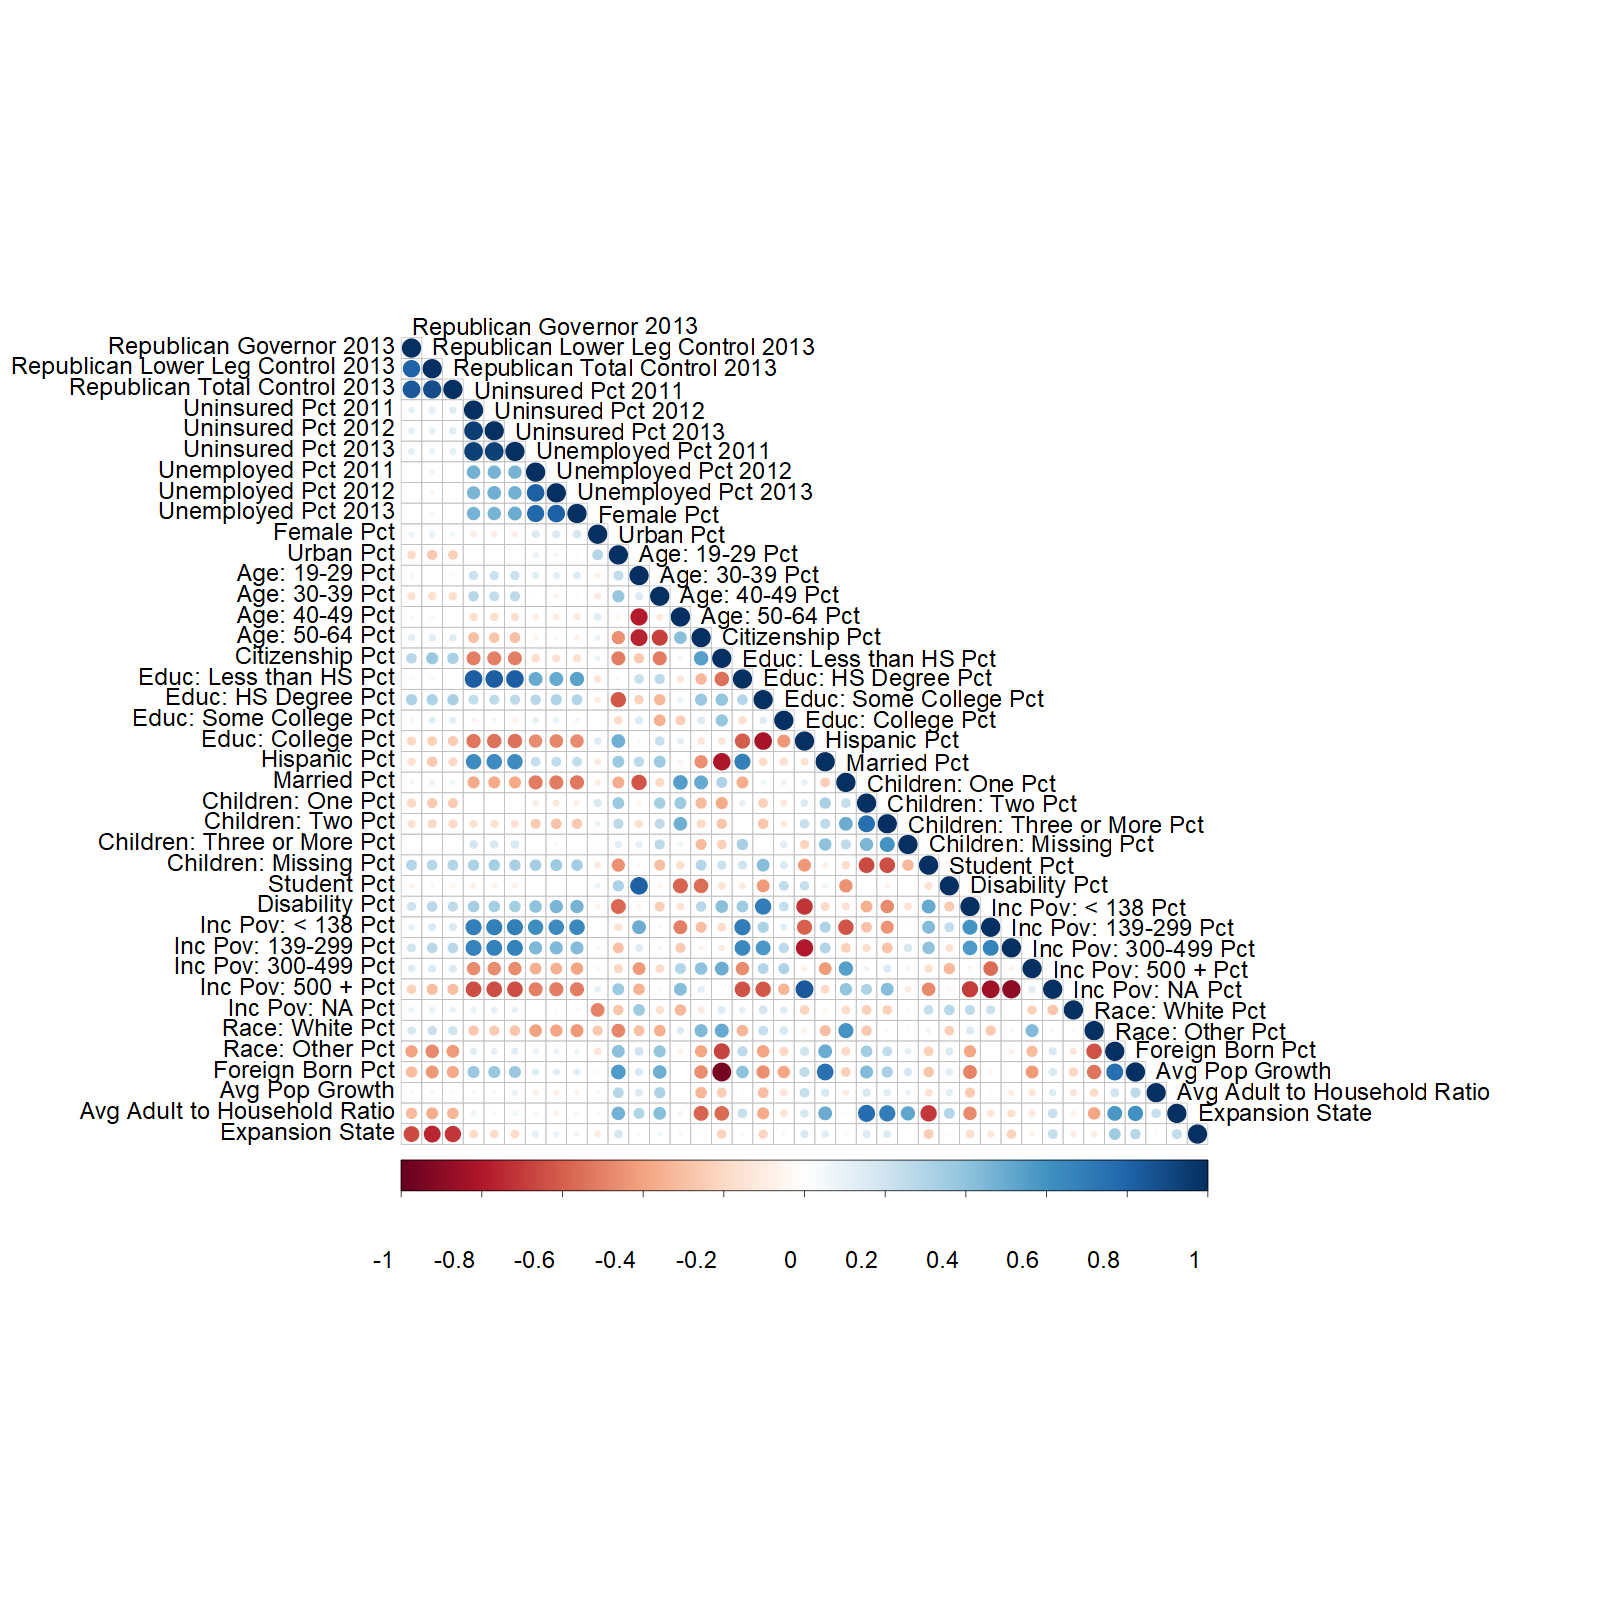
\includegraphics[scale=0.6]{01_Plots/correlation-plot-c1-sigma-zero.png}
\end{center}
\end{figure}

\section{Weight Diagnostics}
\label{ssec:balancetables}

Table~\ref{tab:baltab1} displays the differences between the population-weighted mean covariate values of the non-expansion region and the weighted mean of the expansion region for our primary dataset and with the early expansion states excluded (calculated using our covariate adjustments). The weights presented here are from the H-SBW estimator. The values under each column of ``Primary'' and ``Early Excluded'' are in the following format: (unweighted difference, weighted difference). Additional results are available on request.

\begin{table}[ht]
\centering
    \caption{Balance Table}
    \label{tab:baltab1}
\begin{tabular}{lll}
  \hline
Variables & Preferred & Early Excluded \\ 
  \hline
age\_cat2\_19\_29\_pct & (0.51, 0.50) & (0.77, 0.42) \\ 
  age\_cat2\_30\_39\_pct & (0.23, 0.42) & (0.71, 0.23) \\ 
  age\_cat2\_40\_49\_pct & (-0.10, 0.50) & (0.00, 0.33) \\ 
  avg\_adult\_hh\_ratio & (-10.11, -0.15) & (-2.19, -0.25) \\ 
  citizenship\_pct & (2.19, 2.00) & (-1.18, 1.88) \\ 
  disability\_pct & (1.01, -0.52) & (-0.23, -0.66) \\ 
  educ\_hs\_degree\_pct & (2.38, -1.54) & (0.08, -1.92) \\ 
  educ\_less\_than\_hs\_pct & (0.74, -1.32) & (1.62, -1.52) \\ 
  educ\_some\_college\_pct & (-0.01, -0.75) & (-0.77, -0.54) \\ 
  female\_pct & (0.34, 0.72) & (0.25, 0.95) \\ 
  foreign\_born\_pct & (-5.26, -2) & (1.28, -2.00) \\ 
  hins\_unins\_pct\_2011 & (4.37, -0.05) & (5, -0.05) \\ 
  hins\_unins\_pct\_2012 & (4.10, 0.00) & (4.73, -0.05) \\ 
  hins\_unins\_pct\_2013 & (3.84, 0.05) & (4.16, 0.05) \\ 
  hispanic\_pct & (-1.7, -1.00) & (4.1, -1.00) \\ 
  inc\_pov2\_138\_pct & (1.92, -0.57) & (1.17, 0.61) \\ 
  inc\_pov2\_139\_299\_pct & (2.43, -0.83) & (1.55, -0.4) \\ 
  inc\_pov2\_300\_499\_pct & (0.27, -0.03) & (-0.56, -0.13) \\ 
  inc\_pov2\_500\_plus\_pct & (-5.01, 2.00) & (-2.4, 1.31) \\ 
  married\_pct & (0.68, 0.74) & (0.23, 0.28) \\ 
  missing\_children\_pct & (3.63, 2.08) & (2.34, 1) \\ 
  one\_child\_pct & (-0.53, 0.15) & (0.05, 0.05) \\ 
  pop\_growth\_2012 & (2.55, 0.25) & (4.61, 0.25) \\ 
  pop\_growth\_2013 & (2.49, -0.23) & (4.59, -0.17) \\ 
  race\_white\_pct & (1.49, -1.00) & (-2.7, -1) \\ 
  repub\_gov & (65.02, 17.4) & (55.02, 17.93) \\ 
  repub\_lower\_control & (74.91, 19.37) & (57.24, 16.53) \\ 
  repub\_total\_control & (73.72, 20.00) & (58.2, 20.00) \\ 
  student\_pct & (-0.18, 0.77) & (0.00, 0.85) \\ 
  three\_plus\_child\_pct & (0.00, 0.07) & (0.19, -0.04) \\ 
  two\_child\_pct & (-0.63, 0.35) & (-0.04, 0.21) \\ 
  unemployed\_pct\_2011 & (-0.81, -0.10) & (-0.57, -0.10) \\ 
  unemployed\_pct\_2012 & (-0.85, 0.10) & (-0.67, 0.10) \\ 
  unemployed\_pct\_2013 & (-0.61, 0.10) & (-0.42, 0.10) \\ 
  urban\_pct & (-6.52, 2.00) & (-0.96, 2.00) \\ 
   \hline
\end{tabular}
\end{table}

Table~\ref{tab:oatedist1} displays the difference in means from the overlap region from the control and treated regions on the primary dataset and with the early expansion states excluded. The numbers are displayed as (absolute distance from control region, absolute distance from treated region). These distances are computed using our adjusted datasets. 

\begin{table}[ht]
\centering
    \caption{Overlap region distance from control, treatment regions (1)}
    \label{tab:oatedist1}
\begin{tabular}{lll}
  \hline
Variable & Preferred & Early Excluded \\ 
  \hline
age\_cat2\_19\_29\_pct & (-1.38, -1.09) & (-1.35, -0.79) \\ 
  age\_cat2\_30\_39\_pct & (-0.65, -1.08) & (-0.69, -0.64) \\ 
  age\_cat2\_40\_49\_pct & (0.01, -0.07) & (-0.02, 0.00) \\ 
  avg\_adult\_hh\_ratio & (-3.62, -14.95) & (-3.92, -7.32) \\ 
  citizenship\_pct & (1.72, 5.27) & (2.02, 2.20) \\ 
  disability\_pct & (0.31, 1.77) & (0.40, 0.62) \\ 
  educ\_hs\_degree\_pct & (0.94, 4.51) & (1.04, 2.31) \\ 
  educ\_less\_than\_hs\_pct & (-1.54, -1.26) & (-1.44, -0.29) \\ 
  educ\_some\_college\_pct & (0.27, 0.67) & (0.56, 0.20) \\ 
  female\_pct & (-0.09, 0.27) & (-0.14, 0.12) \\ 
  foreign\_born\_pct & (-2.17, -9.75) & (-2.78, -3.83) \\ 
  hins\_unins\_pct\_2011 & (-6.76, -0.03) & (-6.78, 0.57) \\ 
  hins\_unins\_pct\_2012 & (-3.11, -0.21) & (-3.13, 0.40) \\ 
  hins\_unins\_pct\_2013 & (-0.93, -0.81) & (-0.99, -0.54) \\ 
  hispanic\_pct & (-4.53, -8.9) & (-4.61, -3.18) \\ 
  inc\_pov2\_138\_pct & (-1.37, 0.62) & (-1.29, -0.04) \\ 
  inc\_pov2\_139\_299\_pct & (-1.32, 2.19) & (-1.14, 1.49) \\ 
  inc\_pov2\_300\_499\_pct & (2.42, 1.68) & (2.52, 0.95) \\ 
  inc\_pov2\_500\_plus\_pct & (0.52, -4.72) & (0.13, -2.49) \\ 
  married\_pct & (2.04, 2.48) & (2.30, 2.29) \\ 
  missing\_children\_pct & (-0.70, 2.43) & (-0.65, 1.20) \\ 
  one\_child\_pct & (-0.88, -1.09) & (-0.93, -0.55) \\ 
  pop\_growth\_2012 & (-9.23, 1.76) & (-9.19, 3.86) \\ 
  pop\_growth\_2013 & (-7.66, 1.90) & (-7.65, 4.01) \\ 
  race\_white\_pct & (4.41, 8.25) & (5.11, 4.77) \\ 
  repub\_gov & (-12.46, 52.56) & (-12.5, 42.52) \\ 
  repub\_lower\_control & (-5.28, 69.63) & (-3.69, 53.55) \\ 
  repub\_total\_control & (-17.73, 55.98) & (-16.19, 42.01) \\ 
  student\_pct & (-0.72, -0.82) & (-0.73, -0.65) \\ 
  three\_plus\_child\_pct & (-0.37, -0.21) & (-0.30, 0.04) \\ 
  two\_child\_pct & (0.40, -0.80) & (0.40, -0.22) \\ 
  unemployed\_pct\_2011 & (-0.25, -0.58) & (-0.26, -0.35) \\ 
  unemployed\_pct\_2012 & (-0.72, -0.71) & (-0.76, -0.57) \\ 
  unemployed\_pct\_2013 & (0.25, -0.68) & (0.23, -0.50) \\ 
  urban\_pct & (-5.34, -13.42) & (-5.70, -8.22) \\ 
   \hline
\end{tabular}
\end{table}

Table ~\ref{tab:oatestateweightsc1} displays the sum of CPUMA-level weights within each state for the OATE region, using the preferred covariate adjustment (``sigma\_uu\_i''), as well as no adjustment (``sigma\_zero'') and the secondary adjustment (``sigma\_uu\_avg''). We display all states where the total sum of weights within states is greater than one for any state. The total sum of weights for each set is standardized to sum to 100 for each set of weights. Table ~\ref{tab:oatestateweightsc2} displays the same results with the early expansion states excluded.

\begin{table}[ht]
\centering
\caption{OATE weights summed by state by covariate adjustment, primary dataset}
\label{tab:oatestateweightsc1}
\begin{tabular}{lrrrr}
  \hline
State & Treatment & sigma\_uu\_i & sigma\_uu\_avg & sigma\_zero \\ 
  \hline
OH & 1 & 33.98 & 35.10 & 36.75 \\ 
  MI & 1 & 26.80 & 26.21 & 27.96 \\ 
  AR & 1 & 16.56 & 16.11 & 12.29 \\ 
  PA & 0 & 16.31 & 17.06 & 18.94 \\ 
  MO & 0 & 15.90 & 15.45 & 11.67 \\ 
  WI & 0 & 12.49 & 12.77 & 13.66 \\ 
  FL & 0 & 10.80 & 11.95 & 11.22 \\ 
  AZ & 1 & 9.36 & 8.58 & 8.97 \\ 
  TN & 0 & 7.01 & 7.50 & 5.78 \\ 
  ME & 0 & 6.48 & 6.46 & 6.17 \\ 
  IA & 1 & 4.83 & 5.30 & 5.73 \\ 
  NC & 0 & 4.68 & 3.92 & 4.69 \\ 
  IN & 0 & 4.49 & 4.06 & 5.56 \\ 
  NJ & 1 & 4.30 & 4.18 & 4.57 \\ 
  NE & 0 & 3.95 & 4.83 & 3.84 \\ 
  KS & 0 & 3.25 & 2.25 & 2.81 \\ 
  VA & 0 & 3.11 & 2.24 & 1.79 \\ 
  AL & 0 & 2.48 & 1.80 & 2.31 \\ 
  TX & 0 & 2.40 & 1.92 & 2.85 \\ 
  UT & 0 & 2.32 & 1.72 & 1.82 \\ 
  ND & 1 & 1.98 & 2.25 & 2.13 \\ 
  NM & 1 & 1.41 & 1.63 & 0.89 \\ 
  OK & 0 & 1.35 & 2.17 & 0.81 \\ 
  NV & 1 & 0.77 & 0.65 & 0.71 \\ 
  AK & 0 & 0.71 & 1.13 & 1.55 \\ 
  MT & 0 & 0.66 & 0.66 & 0.62 \\ 
  SC & 0 & 0.47 & 0.47 & 1.00 \\ 
  \hline
\end{tabular}
\end{table}

\begin{table}[ht]
\centering
\caption{OATE weights summed by state by covariate adjustment, early expansion excluded}
\label{tab:oatestateweightsc2}
\begin{tabular}{lrrrr}
  \hline
State & Treatment & sigma\_uu\_i & sigma\_uu\_avg & sigma\_zero \\ 
  \hline
OH & 1 & 34.61 & 35.55 & 36.92 \\ 
  MI & 1 & 27.67 & 27.01 & 28.43 \\ 
  AR & 1 & 16.60 & 16.27 & 12.56 \\ 
  MO & 0 & 16.01 & 15.56 & 11.87 \\ 
  PA & 0 & 15.63 & 16.22 & 17.60 \\ 
  WI & 0 & 13.88 & 14.02 & 14.51 \\ 
  FL & 0 & 10.04 & 11.09 & 10.52 \\ 
  AZ & 1 & 9.39 & 8.58 & 8.88 \\ 
  TN & 0 & 7.17 & 7.80 & 5.83 \\ 
  IA & 1 & 4.92 & 5.73 & 6.15 \\ 
  ME & 0 & 4.90 & 5.05 & 4.92 \\ 
  NC & 0 & 4.80 & 4.02 & 4.94 \\ 
  IN & 0 & 4.54 & 4.15 & 5.95 \\ 
  NE & 0 & 4.37 & 5.24 & 4.34 \\ 
  KS & 0 & 3.83 & 2.74 & 3.12 \\ 
  AL & 0 & 2.91 & 2.14 & 2.54 \\ 
  NV & 1 & 2.83 & 2.45 & 2.96 \\ 
  TX & 0 & 2.81 & 2.23 & 3.17 \\ 
  UT & 0 & 2.62 & 1.98 & 2.13 \\ 
  VA & 0 & 2.10 & 1.41 & 1.45 \\ 
  NM & 1 & 2.07 & 2.60 & 1.95 \\ 
  ND & 1 & 1.92 & 1.81 & 2.14 \\ 
  OK & 0 & 1.39 & 2.29 & 0.82 \\ 
  AK & 0 & 0.68 & 0.99 & 1.34 \\ 
   \hline
\end{tabular}
\end{table}

\section{Additional Results}
\label{ssec:allresults}

Table~\ref{tab:confintmain} displays the point estimates from all estimators as well as confidence intervals calculated either (a) leave-one-state-out jackknife on the adjusted dataset (CI (states)); (b) leave-one-state-out jackknife repeating the entire adjusted leaving each state out (CI (proc)). This table also includes all analyses calculated on a second version of the adjusted data where we use a common $\kappa$ for all values (sigma\_uu\_avg), which is the adjustment suggested by \cite{carroll2006measurement}. Notice that the confidence intervals are identical for ``sigma\_zero'' because this is the unadjusted dataset. ``sigma\_uu\_i'' is our preferred covariate adjustment.

\begin{table}[ht]
\centering
\caption{Primary point estimates and confidence intervals}
\label{tab:confintmain}
\begin{tabular}{llrll}
  \hline
Weight type & Sigma estimate & Psihat & CI (states) & CI (proc) \\ 
  \hline
H-SBW & sigma\_uu\_i & -1.94 & (-3.56, -0.32) & (-3.70, -0.18) \\ 
  H-SBW & sigma\_uu\_avg & -2.02 & (-3.14, -0.91) & (-4.10, 0.05) \\ 
  H-SBW & sigma\_zero & -2.21 & (-3.22, -1.20) & (-3.22, -1.20) \\ 
  BC-HSBW & sigma\_uu\_i & -2.09 & (-3.54, -0.63) & (-3.99, -0.18) \\ 
  BC-HSBW & sigma\_uu\_avg & -2.05 & (-3.20, -0.90) & (-3.83, -0.27) \\ 
  BC-HSBW & sigma\_zero & -2.44 & (-3.40, -1.48) & (-3.4, -1.48) \\ 
  SBW & sigma\_uu\_i & -1.76 & (-3.57, 0.06) & (-3.8, 0.29) \\ 
  SBW & sigma\_uu\_avg & -1.92 & (-3.22, -0.63) & (-4.19, 0.34) \\ 
  SBW & sigma\_zero & -2.20 & (-3.32, -1.07) & (-3.32, -1.07) \\ 
  BC-SBW & sigma\_uu\_i & -1.84 & (-3.03, -0.64) & (-3.57, -0.11) \\ 
  BC-SBW & sigma\_uu\_avg & -1.90 & (-2.77, -1.03) & (-6.65, 2.85) \\ 
  BC-SBW & sigma\_zero & -2.31 & (-3.09, -1.53) & (-3.09, -1.53) \\ 
   \hline
\end{tabular}
\end{table}

Table ~\ref{tab:deltac1} presents the difference in the estimated contrast when excluding the Republican governance indicators along with inferential estimates. Table~\ref{tab:ptests} presents all point estimates from estimators that we calculated. The ``Var subset`` column indicates which variables were excluded from the estimation: 0 excludes no variables; 1 removes Republican governance indicators; 2 pre-treatment uninsurance and unemployment rates; 3 urban, age, education, citizenship, marital status, student, disability, or female; 4 race, ethnicity, income, foreign born; 5 children, population growth, and household to person ratio. We see that the largest changes generally occur when excluding the pre-treatment uninsurance and unemployment rates. This is not surprising: controlling for the other covariates, the pre-treatment uninsurance rate was substantially lower in the treated region compared to the control region. Given that pre-treatment uninsurance rates are highly correlated with post-treatment rates, we find that this comparison leads to a larger absolute magnitude point estimate, highlighting the need to control for these covariates.

\begin{table}[ht]
\centering
\caption{$\hat{\Delta}$ estimates primary dataset}
\label{tab:deltac1}
\begin{tabular}{llrll}
  \hline
Weight type & Sigma estimate & $\hat{\Delta}$ & CI (states) & CI (proc) \\
  \hline
H-SBW & sigma\_uu\_i\_modeled & -0.62 & (-2.05, 0.81) & (-2.21, 0.97) \\ 
  H-SBW & sigma\_uu\_avg & -0.60 & (-1.54, 0.35) & (-2.42, 1.22) \\ 
  H-SBW & sigma\_zero & -0.64 & (-1.62, 0.34) & (-1.62, 0.34) \\ 
  BC-HSBW & sigma\_uu\_i\_modeled & -0.51 & (-1.74, 0.71) & (-2.6, 1.58) \\ 
  BC-HSBW & sigma\_uu\_avg & -0.56 & (-1.44, 0.32) & (-2.84, 1.72) \\ 
  BC-HSBW & sigma\_zero & -0.49 & (-1.33, 0.34) & (-1.33, 0.34) \\ 
  SBW & sigma\_uu\_i\_modeled & -0.92 & (-2.52, 0.67) & (-2.71, 0.86) \\ 
  SBW & sigma\_uu\_avg & -0.79 & (-1.94, 0.37) & (-2.91, 1.34) \\ 
  SBW & sigma\_zero & -0.69 & (-1.67, 0.28) & (-1.67, 0.28) \\ 
  BC-SBW & sigma\_uu\_i\_modeled & -0.41 & (-1.64, 0.82) & (-2.33, 1.51) \\ 
  BC-SBW & sigma\_uu\_avg & -0.32 & (-1.16, 0.53) & (-5.02, 4.39) \\ 
  BC-SBW & sigma\_zero & -0.34 & (-0.98, 0.29) & (-0.98, 0.29) \\ 
   \hline
\end{tabular}
\end{table}

% Wed Jan 13 15:24:43 2021
\begin{table}[ht]
\centering
\caption{Point estimates for all specifications}
\label{tab:ptests}
\begin{tabular}{rlrrrr}
  \hline
Variable subset & Sigma estimate & H-SBW & BC-HSBW & SBW & BC-SBW \\ 
  \hline
0 & sigma\_uu\_i & -1.94 & -2.09 & -1.76 & -1.84 \\ 
  0 & sigma\_uu\_avg & -2.02 & -2.05 & -1.92 & -1.90 \\ 
  0 & sigma\_zero & -2.21 & -2.44 & -2.20 & -2.31 \\ 
  1 & sigma\_uu\_i & -2.56 & -2.60 & -2.68 & -2.25 \\ 
  1 & sigma\_uu\_avg & -2.62 & -2.61 & -2.71 & -2.22 \\ 
  1 & sigma\_zero & -2.84 & -2.93 & -2.89 & -2.66 \\ 
  2 & sigma\_uu\_i & -5.54 & -4.37 & -5.14 & -4.08 \\ 
  2 & sigma\_uu\_avg & -5.61 & -4.35 & -5.28 & -4.08 \\ 
  2 & sigma\_zero & -5.55 & -5.41 & -5.14 & -5.10 \\ 
  3 & sigma\_uu\_i & -1.98 & -2.11 & -1.87 & -1.90 \\ 
  3 & sigma\_uu\_avg & -1.98 & -2.02 & -1.85 & -1.84 \\ 
  3 & sigma\_zero & -2.10 & -1.94 & -2.17 & -1.94 \\ 
  4 & sigma\_uu\_i & -2.14 & -2.12 & -1.89 & -1.83 \\ 
  4 & sigma\_uu\_avg & -2.37 & -2.07 & -2.31 & -1.99 \\ 
  4 & sigma\_zero & -2.18 & -2.45 & -2.14 & -2.32 \\ 
  5 & sigma\_uu\_i & -1.75 & -2.28 & -1.78 & -2.16 \\ 
  5 & sigma\_uu\_avg & -1.97 & -2.43 & -2.00 & -2.36 \\ 
  5 & sigma\_zero & -2.08 & -2.38 & -2.18 & -2.38 \\ 
   \hline
\end{tabular}
\end{table}

Table ~\ref{tab:confintmainc2}, Table~\ref{tab:deltac2}, and Table~\ref{tab:secondaryptests} are identical to the structure of the previous two tables except we exclude the ``early expansion states'' from the pool of expansion state matches. 

\begin{table}[ht]
\centering
\caption{Early expansion excluded, point estimates and confidence intervals}
\label{tab:confintmainc2}
\begin{tabular}{llrll}
  \hline
Weight type & Sigma estimate & Psihat & CI (states) & CI (proc) \\ 
  \hline
H-SBW & sigma\_uu\_i & -1.43 & (-2.88, 0.02) & (-3.14, 0.28) \\ 
  H-SBW & sigma\_uu\_avg & -1.88 & (-3.49, -0.27) & (-4.24, 0.47) \\ 
  H-SBW & sigma\_zero & -1.77 & (-2.62, -0.93) & (-2.62, -0.93) \\ 
  BC-HSBW & sigma\_uu\_i & -2.01 & (-3.68, -0.33) & (-3.6, -0.41) \\ 
  BC-HSBW & sigma\_uu\_avg & -2.38 & (-4.20, -0.56) & (-4.87, 0.11) \\ 
  BC-HSBW & sigma\_zero & -2.47 & (-3.64, -1.30) & (-3.64, -1.30) \\ 
  SBW & sigma\_uu\_i & -1.17 & (-2.86, 0.51) & (-2.96, 0.62) \\ 
  SBW & sigma\_uu\_avg & -1.84 & (-2.94, -0.74) & (-4.09, 0.42) \\ 
  SBW & sigma\_zero & -1.71 & (-2.62, -0.79) & (-2.62, -0.79) \\ 
  BC-SBW & sigma\_uu\_i & -1.69 & (-3.39, 0.01) & (-3.1, -0.28) \\ 
  BC-SBW & sigma\_uu\_avg & -2.22 & (-3.81, -0.63) & (-4.61, 0.17) \\ 
  BC-SBW & sigma\_zero & -2.37 & (-3.71, -1.02) & (-3.71, -1.02) \\ 
   \hline
\end{tabular}
\end{table}

\begin{table}[ht]
\centering
\caption{$\hat{\Delta}$ estimates, early expansion excluded}
\label{tab:deltac2}
\begin{tabular}{llrll}
  \hline
Weight type & Sigma estimate & $\hat{\Delta}$ & CI (state) & CI (proc) \\ 
  \hline
H-SBW & sigma\_uu\_i\_modeled & -1.15 & (-2.53, 0.24) & (-2.5, 0.2) \\ 
  H-SBW & sigma\_uu\_avg & -0.72 & (-2.22, 0.78) & (-3.01, 1.58) \\ 
  H-SBW & sigma\_zero & -1.04 & (-2.01, -0.07) & (-2.01, -0.07) \\ 
  BC-HSBW & sigma\_uu\_i\_modeled & -0.74 & (-2.4, 0.91) & (-2.23, 0.75) \\ 
  BC-HSBW & sigma\_uu\_avg & -0.39 & (-1.97, 1.19) & (-2.66, 1.89) \\ 
  BC-HSBW & sigma\_zero & -0.61 & (-1.75, 0.52) & (-1.75, 0.52) \\ 
  SBW & sigma\_uu\_i\_modeled & -1.46 & (-2.9, -0.02) & (-2.84, -0.08) \\ 
  SBW & sigma\_uu\_avg & -0.83 & (-1.86, 0.2) & (-2.88, 1.22) \\ 
  SBW & sigma\_zero & -1.06 & (-2.12, 0) & (-2.12, 0) \\ 
  BC-SBW & sigma\_uu\_i\_modeled & -0.86 & (-2.37, 0.65) & (-2.16, 0.44) \\ 
  BC-SBW & sigma\_uu\_avg & -0.33 & (-1.58, 0.92) & (-2.31, 1.65) \\ 
  BC-SBW & sigma\_zero & -0.40 & (-1.92, 1.11) & (-1.92, 1.11) \\ 
   \hline
\end{tabular}
\end{table}

\begin{table}[ht]
\centering
   \caption{Point estimates for all specifications, early expansion excluded}
    \label{tab:secondaryptests}
\begin{tabular}{rlrrrr}
  \hline
Variable subset & Sigma estimate & H-SBW & BC-HSBW & SBW & BC-SBW \\ 
  \hline
0 & sigma\_uu\_i & -1.43 & -2.01 & -1.17 & -1.69 \\ 
  0 & sigma\_uu\_avg & -1.88 & -2.38 & -1.84 & -2.22 \\ 
  0 & sigma\_zero & -1.77 & -2.47 & -1.71 & -2.37 \\ 
  1 & sigma\_uu\_i & -2.57 & -2.75 & -2.63 & -2.55 \\ 
  1 & sigma\_uu\_avg & -2.60 & -2.77 & -2.67 & -2.55 \\ 
  1 & sigma\_zero & -2.81 & -3.08 & -2.77 & -2.77 \\ 
  2 & sigma\_uu\_i & -5.48 & -4.38 & -4.96 & -4.23 \\ 
  2 & sigma\_uu\_avg & -5.55 & -4.42 & -5.06 & -4.26 \\ 
  2 & sigma\_zero & -5.47 & -5.25 & -4.95 & -5.09 \\ 
  3 & sigma\_uu\_i & -1.41 & -1.81 & -1.19 & -1.67 \\ 
  3 & sigma\_uu\_avg & -1.87 & -2.16 & -1.83 & -2.01 \\ 
  3 & sigma\_zero & -1.71 & -1.76 & -1.70 & -1.69 \\ 
  4 & sigma\_uu\_i & -1.86 & -2.01 & -1.75 & -1.66 \\ 
  4 & sigma\_uu\_avg & -2.21 & -2.35 & -1.93 & -1.97 \\ 
  4 & sigma\_zero & -1.87 & -2.49 & -1.90 & -2.35 \\ 
  5 & sigma\_uu\_i & -1.38 & -2.15 & -1.18 & -1.90 \\ 
  5 & sigma\_uu\_avg & -1.29 & -2.10 & -1.21 & -2.07 \\ 
  5 & sigma\_zero & -1.67 & -2.22 & -1.53 & -2.09 \\ 
   \hline
\end{tabular}
\end{table}

Table~\ref{tab:loostatec1} and Table~\ref{tab:loostatec2} present point estimates for the leave-one-state out analysis for our preferred estimator, H-SBW calculated on our preferred covariate adjustment for the primary dataset and when excluding early expansion states.

\begin{table}[ht]
\centering
   \caption{Leave-one-state-out point estimates, primary dataset, preferred adjustment}
    \label{tab:loostatec1}
\begin{tabular}{lrlrl}
  \hline
State & Psihat (0) & None (states, proc) & Psihat (1) & Repub (states, proc) \\ 
  \hline
AR & -1.94 & (-2.13, -2.15) & -2.56 & (-2.5, -2.5) \\ 
  AZ & -1.94 & (-2.07, -2.01) & -2.56 & (-2.60, -2.60) \\ 
  CA & -1.94 & (-1.41, -1.31) & -2.56 & (-2.52, -2.46) \\ 
  CO & -1.94 & (-1.94, -1.95) & -2.56 & (-2.62, -2.61) \\ 
  CT & -1.94 & (-1.94, -1.94) & -2.56 & (-2.56, -2.51) \\ 
  HI & -1.94 & (-1.94, -1.91) & -2.56 & (-2.49, -2.5) \\ 
  IA & -1.94 & (-1.82, -1.85) & -2.56 & (-2.58, -2.57) \\ 
  IL & -1.94 & (-1.95, -1.88) & -2.56 & (-2.55, -2.56) \\ 
  KY & -1.94 & (-1.86, -1.80) & -2.56 & (-2.34, -2.21) \\ 
  MD & -1.94 & (-1.97, -2.06) & -2.56 & (-2.63, -2.66) \\ 
  MI & -1.94 & (-1.57, -1.61) & -2.56 & (-2.56, -2.58) \\ 
  MN & -1.94 & (-1.94, -1.88) & -2.56 & (-2.58, -2.6) \\ 
  ND & -1.94 & (-2.00, -2.04) & -2.56 & (-2.57, -2.59) \\ 
  NH & -1.94 & (-1.94, -1.97) & -2.56 & (-2.68, -2.66) \\ 
  NJ & -1.94 & (-2.13, -2.09) & -2.56 & (-2.68, -2.73) \\ 
  NM & -1.94 & (-1.89, -1.96) & -2.56 & (-2.44, -2.43) \\ 
  NV & -1.94 & (-1.94, -2.02) & -2.56 & (-2.60, -2.60) \\ 
  OH & -1.94 & (-2.33, -2.35) & -2.56 & (-2.78, -2.72) \\ 
  OR & -1.94 & (-1.92, -2.02) & -2.56 & (-2.51, -2.52) \\ 
  RI & -1.94 & (-1.94, -1.91) & -2.56 & (-2.54, -2.52) \\ 
  WA & -1.94 & (-1.85, -1.89) & -2.56 & (-2.46, -2.39) \\ 
  WV & -1.94 & (-1.94, -1.96) & -2.56 & (-2.48, -2.49) \\ 
   \hline
\end{tabular}
\end{table}

\begin{table}[ht]
\centering
   \caption{Leave-one-state-out point estimates, early expansion excluded, preferred adjustment}
    \label{tab:loostatec2}
\begin{tabular}{lrlrl}
  \hline
State & Psihat (0) & None (states, proc) & Psihat (1) & Repub (states, proc) \\ 
  \hline
AR & -1.43 & (-1.47, -1.43) & -2.57 & (-2.43, -2.43) \\ 
  AZ & -1.43 & (-1.59, -1.53) & -2.57 & (-2.61, -2.6) \\ 
  CO & -1.43 & (-1.43, -1.36) & -2.57 & (-2.58, -2.55) \\ 
  HI & -1.43 & (-1.43, -1.43) & -2.57 & (-2.44, -2.46) \\ 
  IA & -1.43 & (-1.31, -1.33) & -2.57 & (-2.6, -2.58) \\ 
  IL & -1.43 & (-1.37, -1.49) & -2.57 & (-2.49, -2.48) \\ 
  KY & -1.43 & (-1.38, -1.05) & -2.57 & (-2.35, -2.23) \\ 
  MD & -1.43 & (-1.7, -1.61) & -2.57 & (-2.64, -2.63) \\ 
  MI & -1.43 & (-0.98, -0.95) & -2.57 & (-2.56, -2.59) \\ 
  ND & -1.43 & (-1.78, -1.8) & -2.57 & (-2.57, -2.57) \\ 
  NH & -1.43 & (-1.43, -1.6) & -2.57 & (-2.72, -2.71) \\ 
  NM & -1.43 & (-1.42, -1.3) & -2.57 & (-2.34, -2.32) \\ 
  NV & -1.43 & (-1.55, -1.54) & -2.57 & (-2.72, -2.72) \\ 
  OH & -1.43 & (-1.77, -1.81) & -2.57 & (-2.77, -2.75) \\ 
  OR & -1.43 & (-1.42, -1.57) & -2.57 & (-2.55, -2.56) \\ 
  RI & -1.43 & (-1.43, -1.45) & -2.57 & (-2.56, -2.55) \\ 
  WV & -1.43 & (-1.43, -1.41) & -2.57 & (-2.49, -2.49) \\ 
   \hline
\end{tabular}
\end{table}

Finally, Figure~\ref{fig:rdiffc1state}, Figure~\ref{fig:rdiffc1proc}, Figure~\ref{fig:rdiffc2state}, and Figure~\ref{fig:rdiffc2proc} display heatmaps showing the estimates of $\hat{\Delta}$ for all of our estimators when removing each state. We see that these estimates are overwhelmingly negative. We only estimate positive contrasts on our primary dataset when recalculating the covariate adjustment excluding that state and when the estimator could extrapolate beyond the support of the data. For the primary dataset, this occurred with California and Illinois. When removing early expansion states this only occurred when removing Hawaii and Ohio for our less preferred covariate adjustment.

We also caution against over-interpreting those particular estimates: as we noted in Appendix C, the covariate adjustments can result in estimates that are outside of the support of the data, or even possible values. While quite rare on our primary dataset, these bad estimates occur more frequently when we recalculate the adjustment when removing each state. In general, we expect estimators that do not extrapolate to be less affected by these bad adjustments, since they will likely get close to no weight; however, estimators that extrapolate are more likely to use the data from these CPUMAs, resulting in dubious estimates. 

\begin{figure}[]
\begin{center}
    \caption{$\hat{\Delta}$ leave-one-out state, primary dataset, covariate adjustment constant}
    \label{fig:rdiffc1state}
    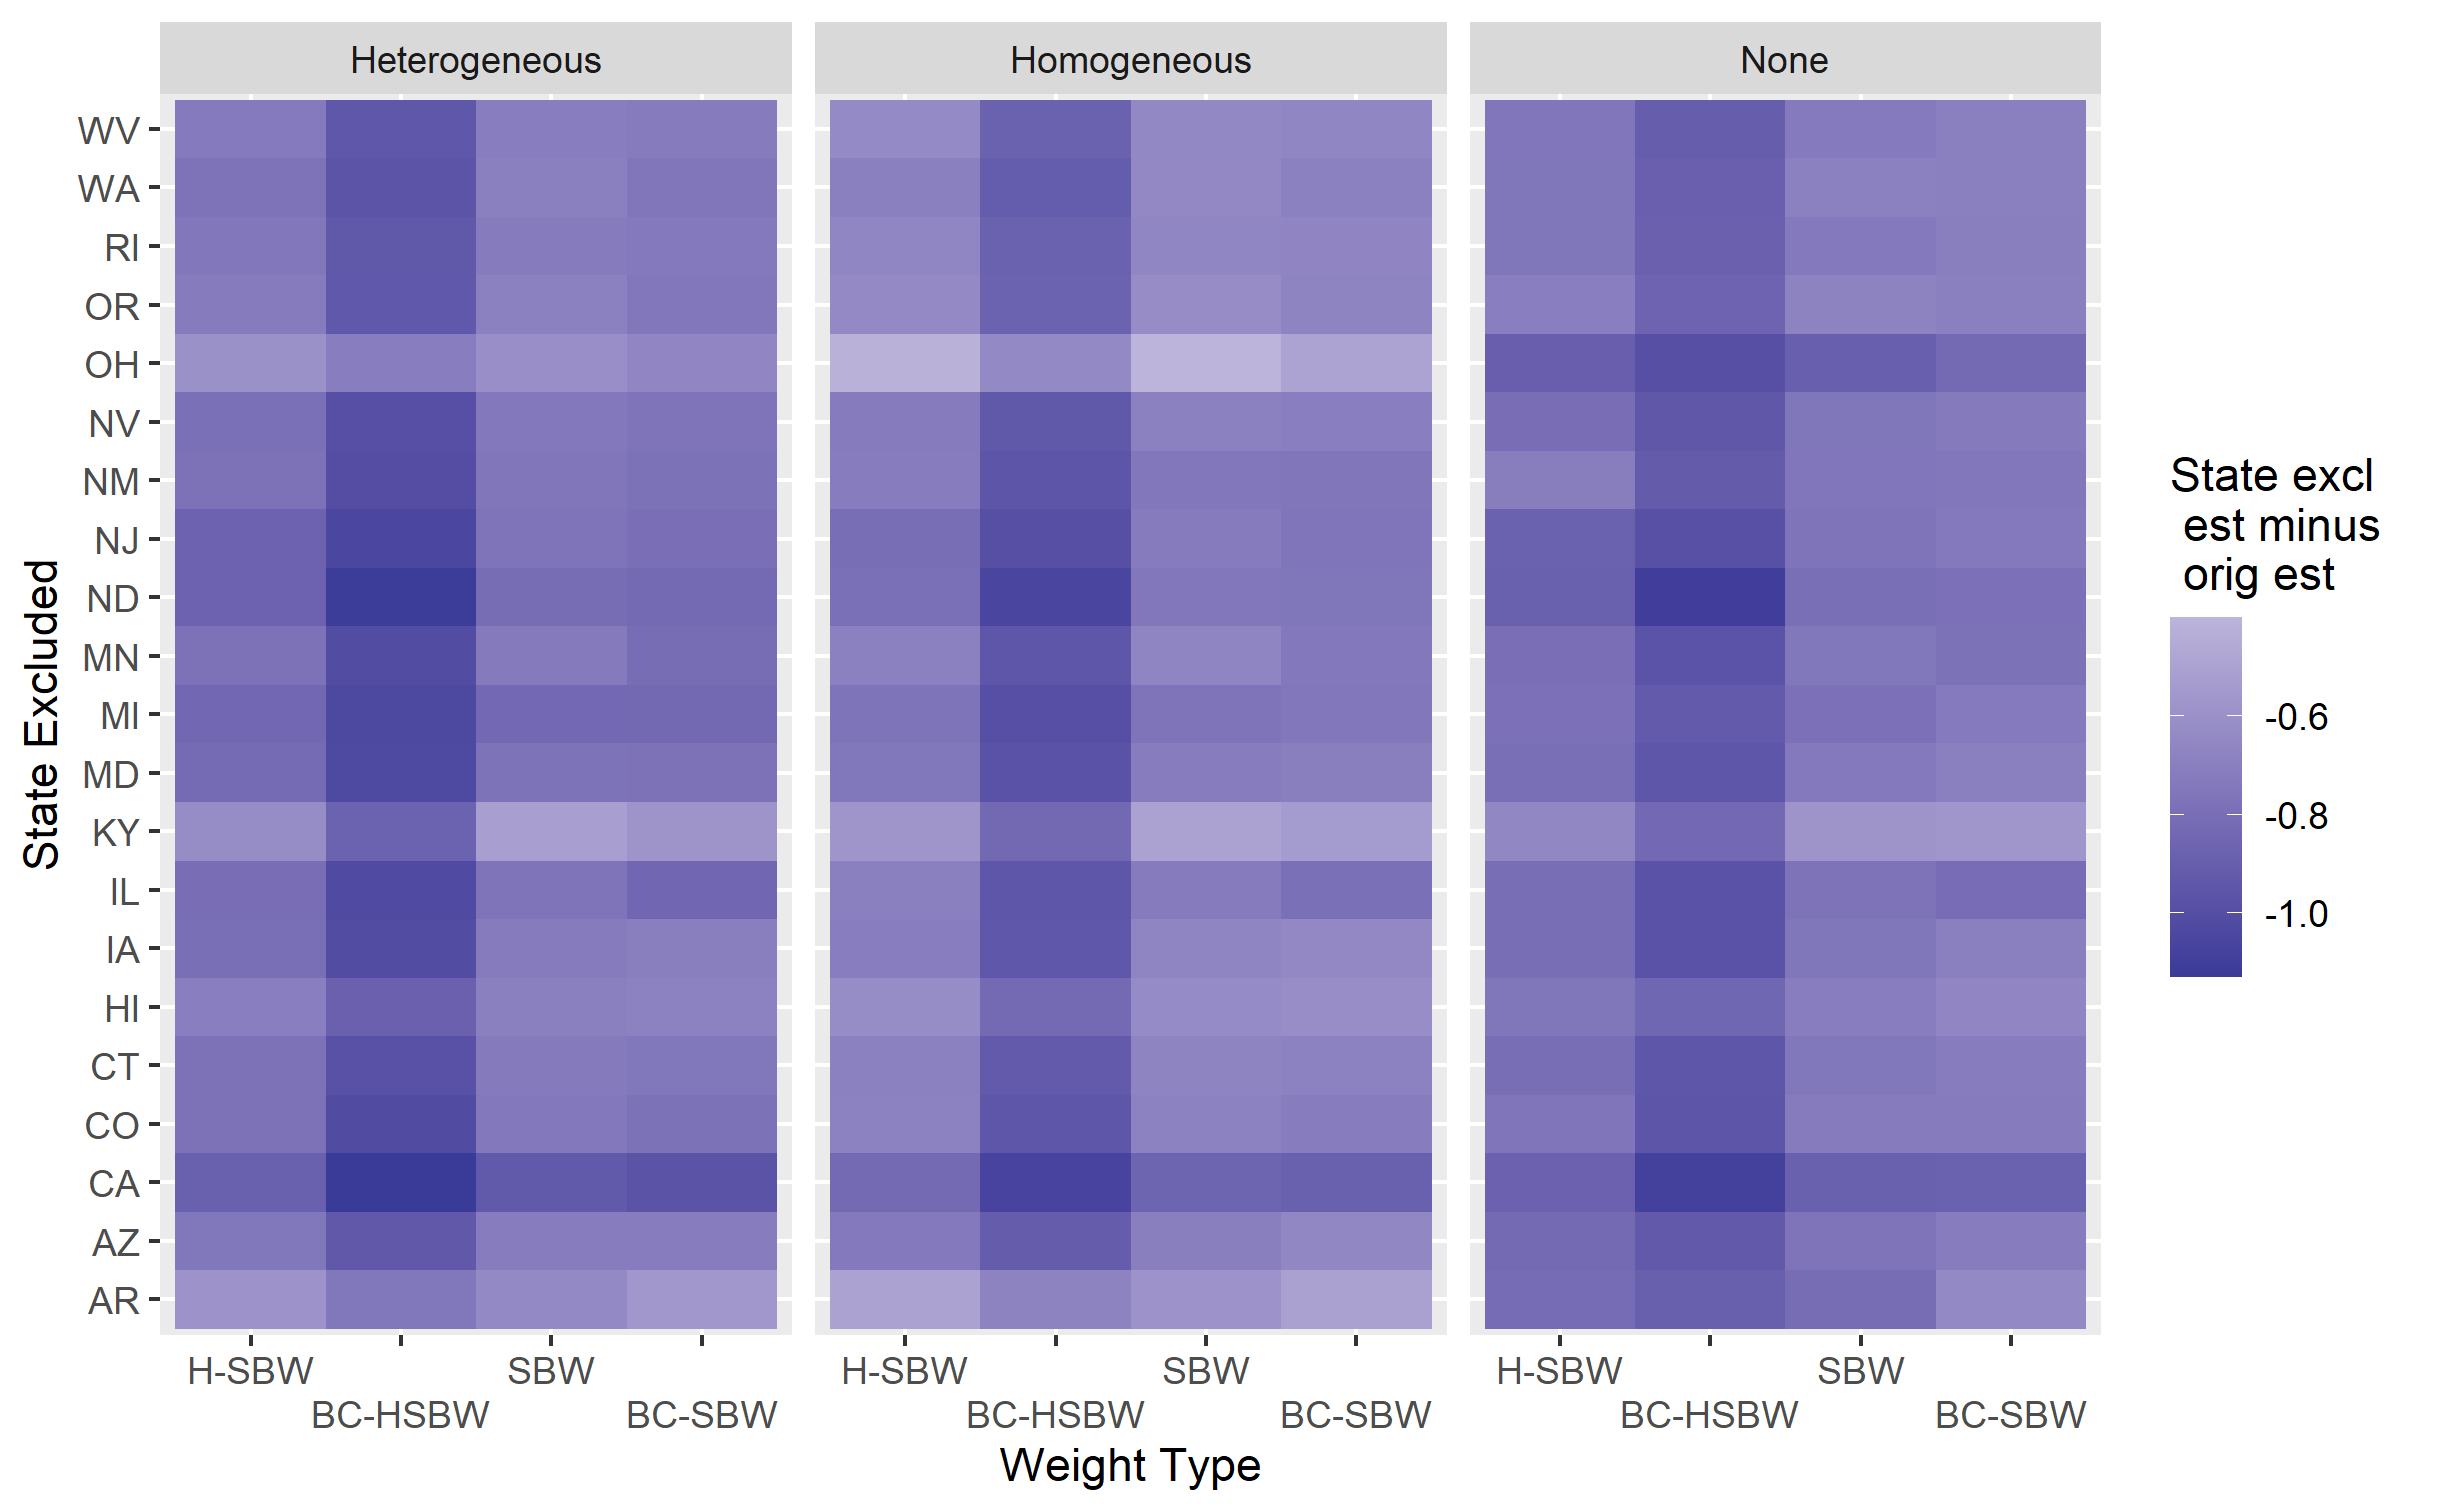
\includegraphics[scale=0.6]{01_Plots/loostate-repub-sensitivityc1-state-main.png}
\end{center}
\end{figure}

\begin{figure}[]
\begin{center}
    \caption{$\hat{\Delta}$ leave-one-out state, primary dataset, covariate adjustment recalculated}
    \label{fig:rdiffc1proc}
    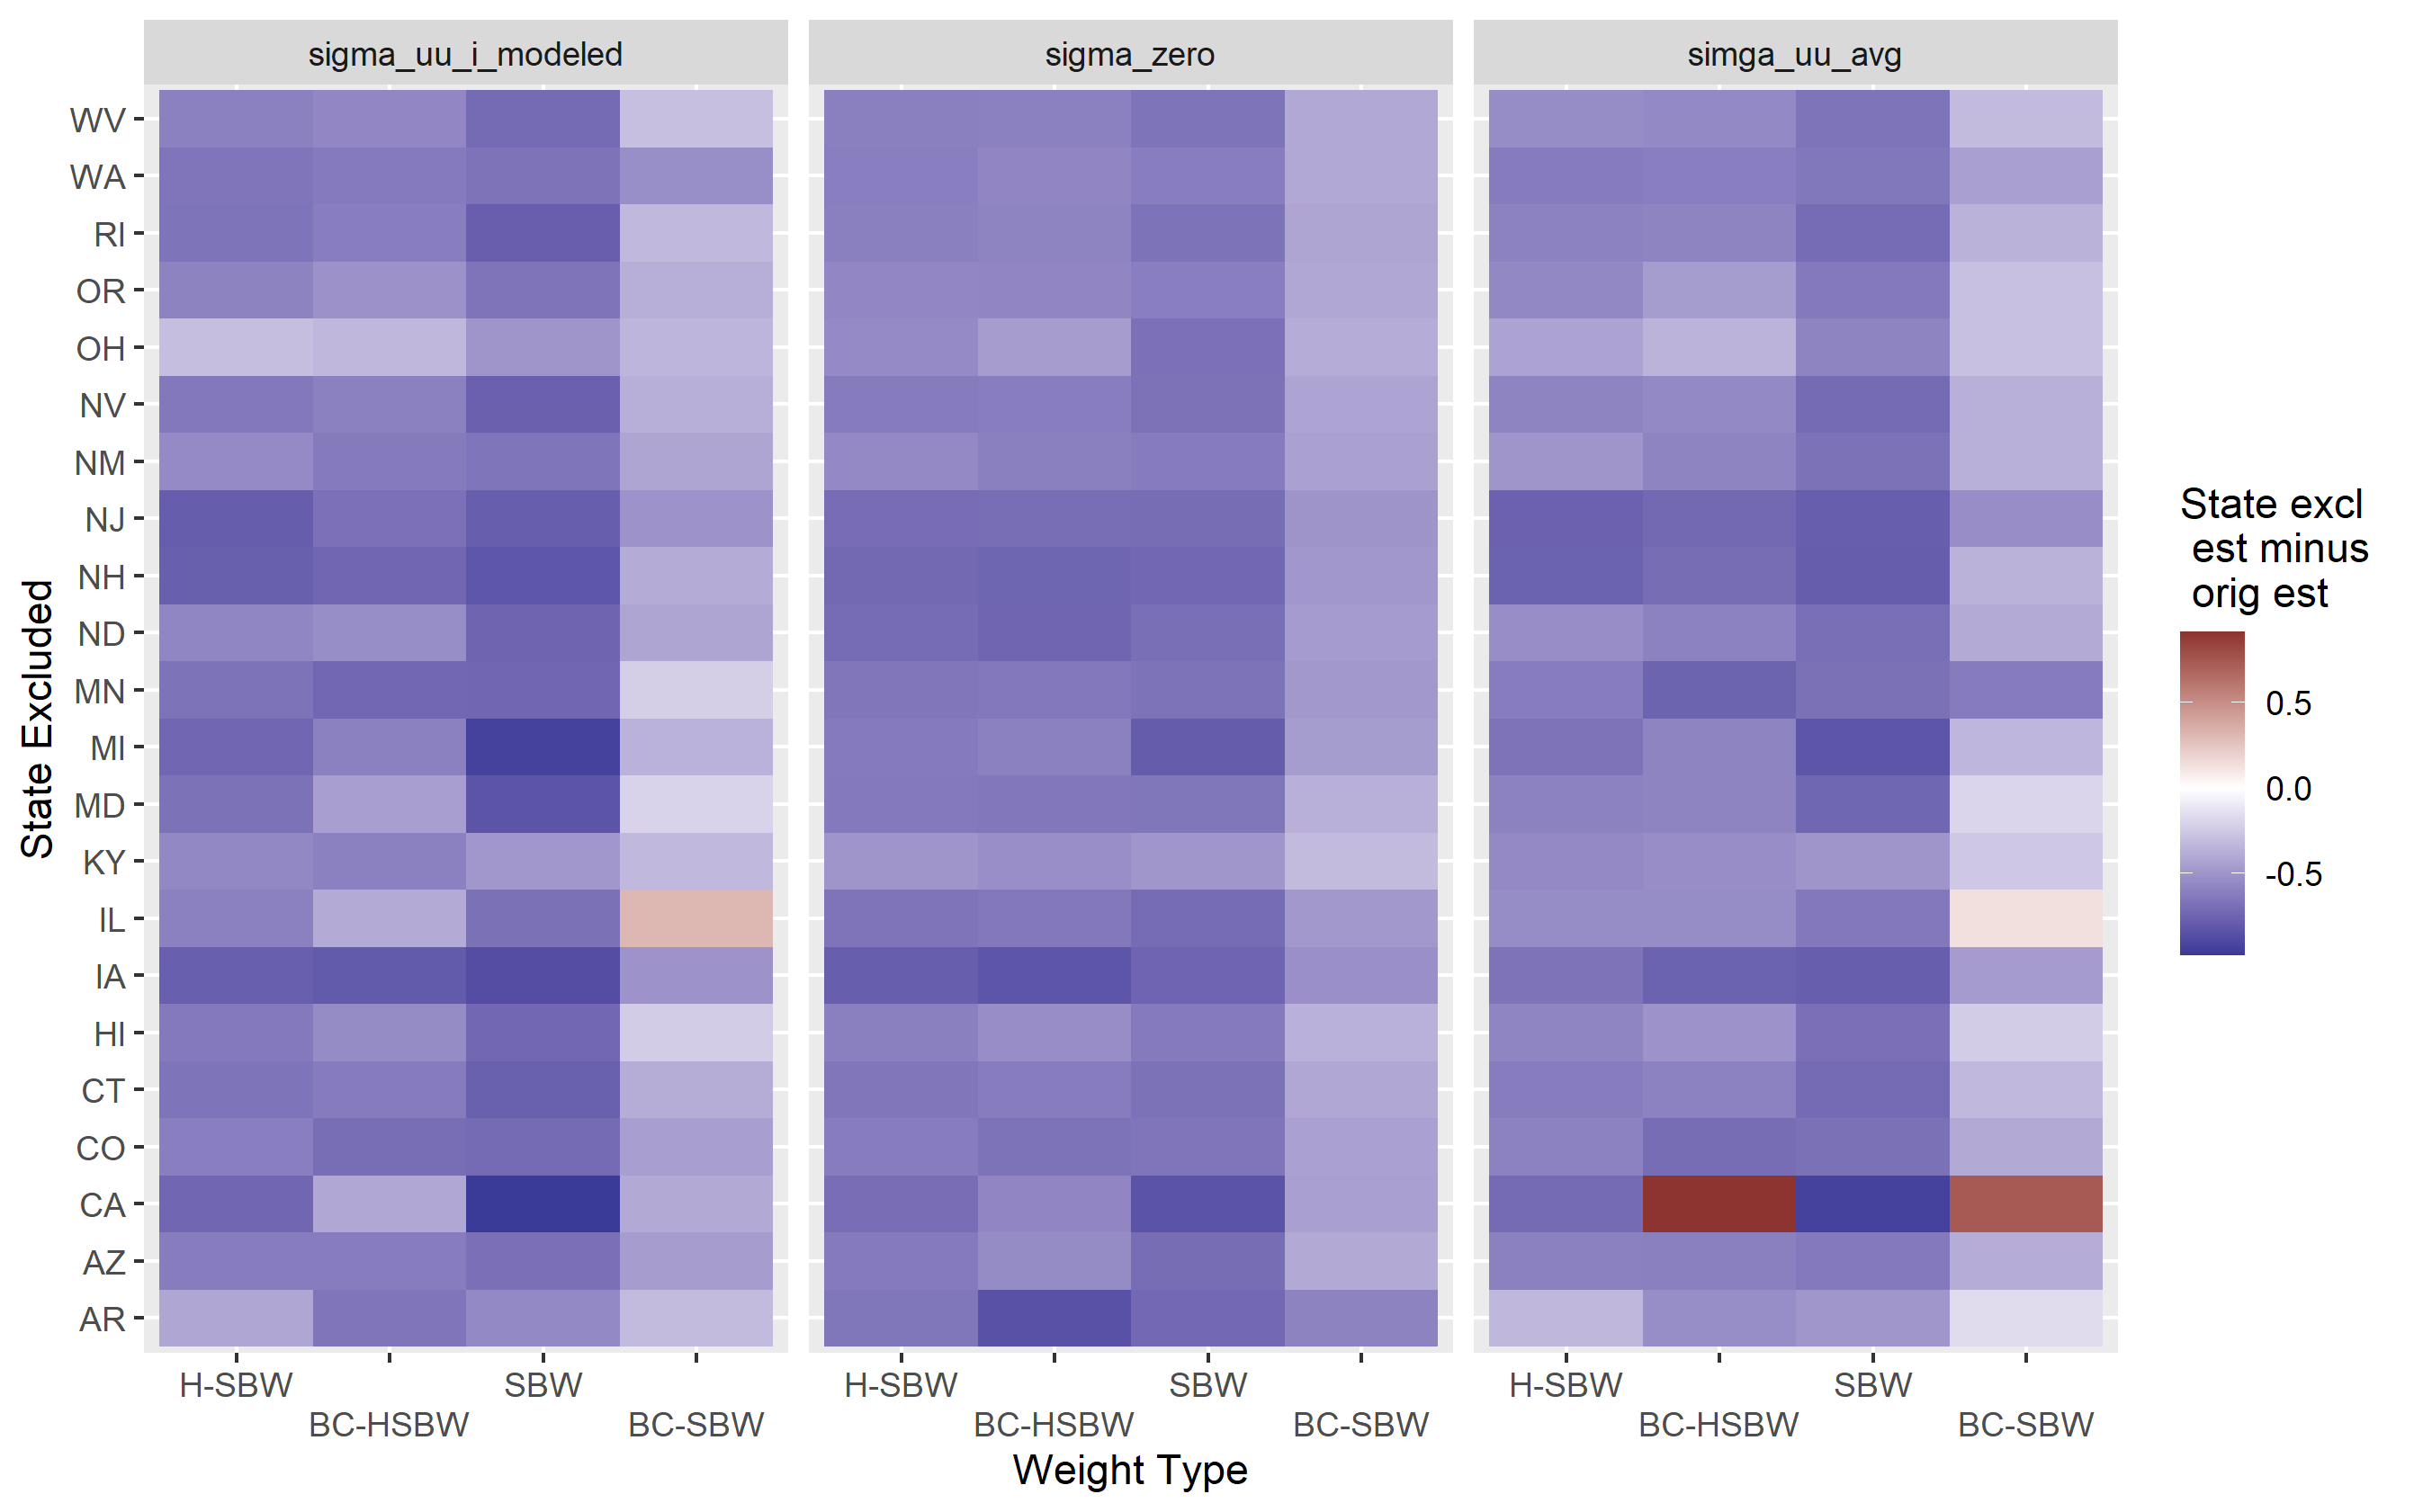
\includegraphics[scale=0.6]{01_Plots/loostate-repub-sensitivityc1-proc-main.png}
\end{center}
\end{figure}

\begin{figure}[]
\begin{center}
    \caption{$\hat{\Delta}$ leave-one-out state, early expansion excluded, covariate adjustment constant}
    \label{fig:rdiffc2state}
    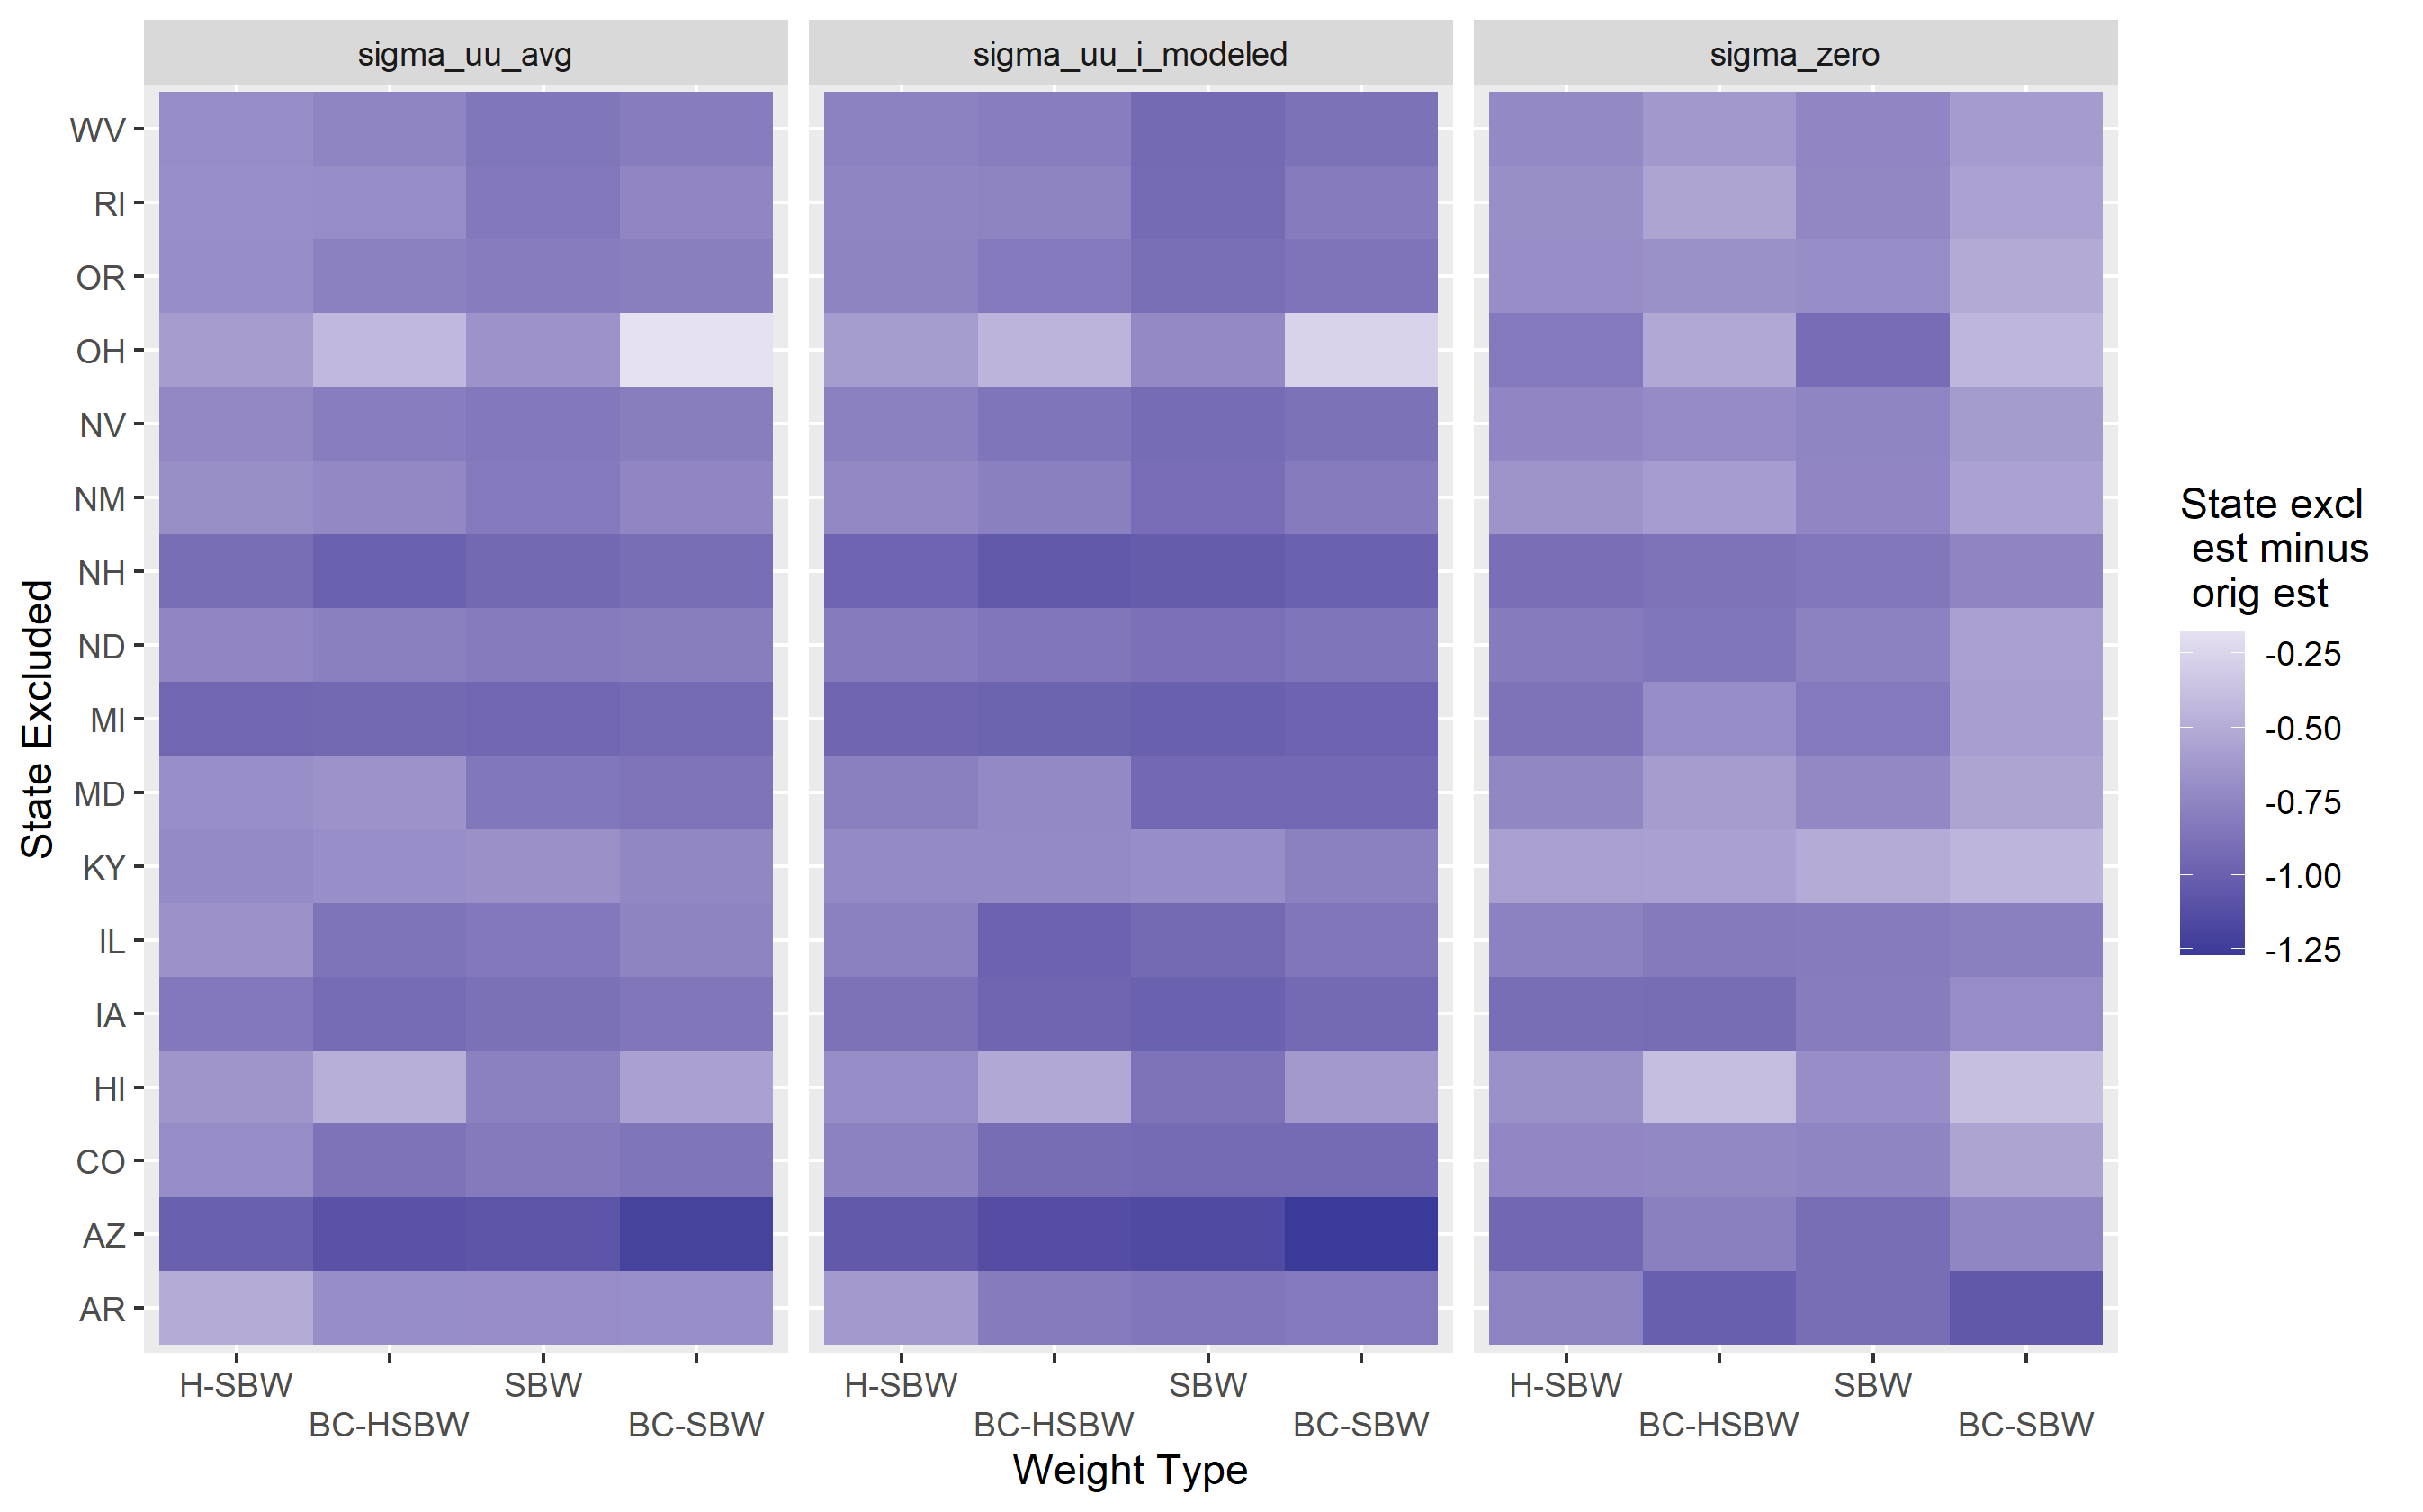
\includegraphics[scale=0.6]{01_Plots/loostate-repub-sensitivityc2-state-main.png}
\end{center}
\end{figure}

\begin{figure}[]
\begin{center}
    \caption{$\hat{\Delta}$ leave-one-out state, early expansion excluded, covariate adjustment recalculated}
    \label{fig:rdiffc2proc}
    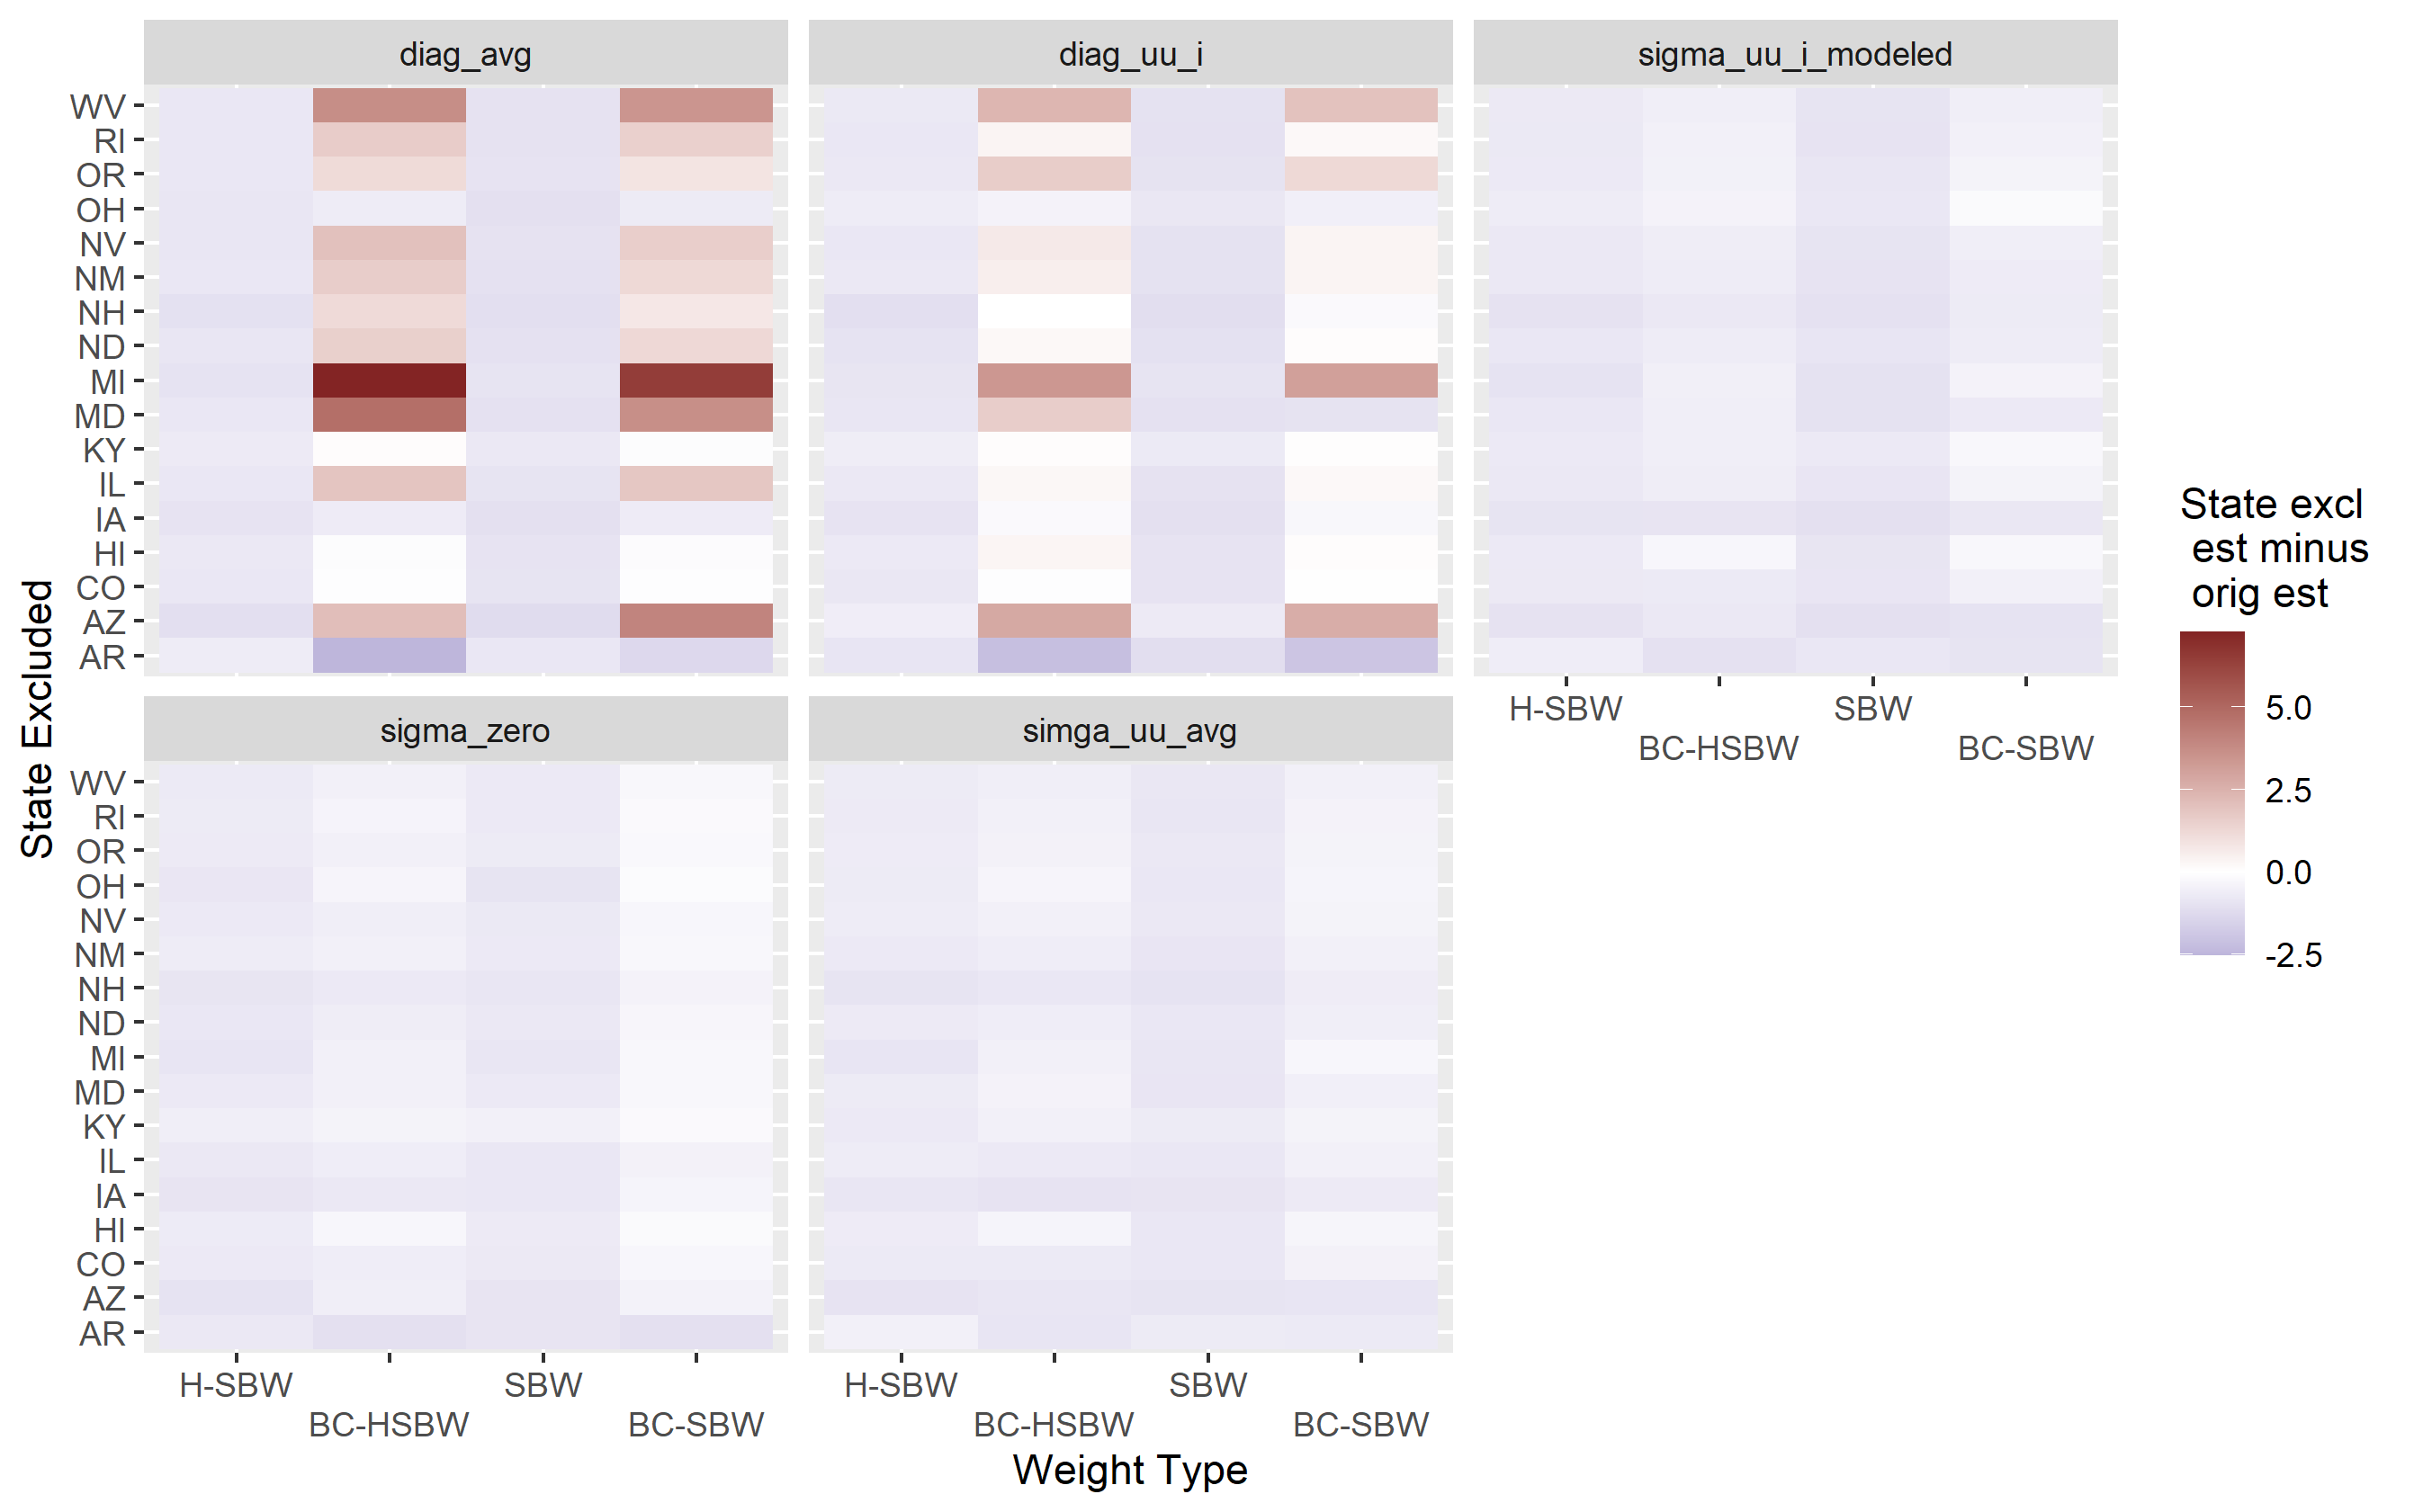
\includegraphics[scale=0.6]{01_Plots/loostate-repub-sensitivityc2-proc-main.png}
\end{center}
\end{figure}

Table~\ref{tab:oateconfint} displays point estimates and confidence intervals for the primary point estimates for the OATE. We display the confidence intervals calculated using both the leave-one-out-states conditional on the covariate adjustment (CI (states)) and recalculating the covariate adjustment for the OATE (CI (proc)). We note that when calculating these confidence intervals, on the rare occasions when logistic regression failed to converge, we used the probit link instead.

\begin{table}[ht]
\centering
\caption{OATE primary results inference}
\label{tab:oateconfint}
\begin{tabular}{rllll}
  \hline
Psihat & Sigma estimate & Dataset & CI (states) & CI (proc) \\ 
  \hline
-1.64 & sigma\_uu\_i & c1 & (-2.40, -0.89) & (-2.57, -0.72) \\ 
  -1.58 & sigma\_avg & c1 & (-2.17, -1.00) & (-2.37, -0.79) \\ 
  -1.80 & sigma\_zero & c1 & (-2.49, -1.10) & (-2.49, -1.10) \\ 
  -1.81 & sigma\_uu\_i & c2 & (-2.47, -1.15) & (-2.63, -0.98) \\ 
  -1.74 & sigma\_avg & c2 & (-2.28, -1.20) & (-2.44, -1.04) \\ 
  -1.95 & sigma\_zero & c2 & (-2.65, -1.25) & (-2.65, -1.25) \\ 
   \hline
\end{tabular}
\end{table}

Table~\ref{tab:oaterepubdiff} displays the difference between the estimated contrasts when excluding Republican governance indicators and when including all covariates as well as the estimated confidence intervals, estimated both conditional on the imputation (CI (states)) and recalculating the entire covariate adjustment (CI (proc)).

\begin{table}[ht]
\centering
\caption{OATE $\hat{\Delta}$ estimates}
\label{tab:oaterepubdiff}
\begin{tabular}{llrll}
  \hline
Sigma estimate & Dataset & $\hat{\Delta}$ & CI (states) & CI (proc) \\ 
  \hline
sigma\_uu\_i & c1 & -0.96 & (-1.11, -0.81) & (-1.12, -0.80) \\ 
  sigma\_uu\_i & c2 & -0.72 & (-0.87, -0.57) & (-0.89, -0.55) \\ 
  sigma\_avg & c1 & -1.04 & (-1.19, -0.89) & (-1.22, -0.86) \\ 
  sigma\_avg & c2 & -0.80 & (-0.98, -0.63) & (-0.99, -0.61) \\ 
  sigma\_zero & c1 & -0.75 & (-0.88, -0.63) & (-0.88, -0.63) \\ 
  sigma\_zero & c2 & -0.56 & (-0.69, -0.43) & (-0.69, -0.43) \\ 
   \hline
\end{tabular}
\end{table}

Table~\ref{tab:oatesensitive} presents all point estimates calculate using the overlap weights. Dataset ``c1'' refers to the primary dataset and dataset ``c2'' removes the early expansion states. The numeric column names refer to the covariate group excluded (covariate groups described above).

\begin{table}[ht]
\centering
\caption{OATE all point estimates}
\label{tab:oatesensitive}
\begin{tabular}{llrrrrrr}
  \hline
Sigma estimate & Dataset & 0 & 1 & 2 & 3 & 4 & 5 \\ 
  \hline
sigma\_uu\_i & c1 & -1.64 & -2.60 & -2.96 & -1.86 & -1.86 & -1.77 \\ 
  sigma\_uu\_i & c2 & -1.81 & -2.53 & -3.10 & -2.18 & -2.04 & -1.96 \\ 
  sigma\_avg & c1 & -1.58 & -2.62 & -2.85 & -1.76 & -1.76 & -1.78 \\ 
  sigma\_avg & c2 & -1.74 & -2.54 & -3.00 & -2.10 & -1.96 & -1.95 \\ 
  sigma\_zero & c1 & -1.80 & -2.55 & -3.11 & -1.98 & -1.94 & -1.83 \\ 
  sigma\_zero & c2 & -1.95 & -2.51 & -3.25 & -2.12 & -2.10 & -2.00 \\ 
   \hline
\end{tabular}
\end{table}

Figure~\ref{fig:oateheatmap} displays a heatmap showing how the OATE point estimates change when removing each state, conditional on our preferred covariate adjustment for both the primary dataset and when excluding early expansion states. We present the results for all covariates and excluding the Republican governance indicators. Additional results are available on request. We see that our point estimates move closer to zero when removing Wisconsin or Ohio for all specifications. Removing Arkansas appears to generally move the point estimates further away from zero.

\begin{figure}[]
\begin{center}
    \caption{OATE estimates, leave-one-out-states analysis}
    \label{fig:oateheatmap}
    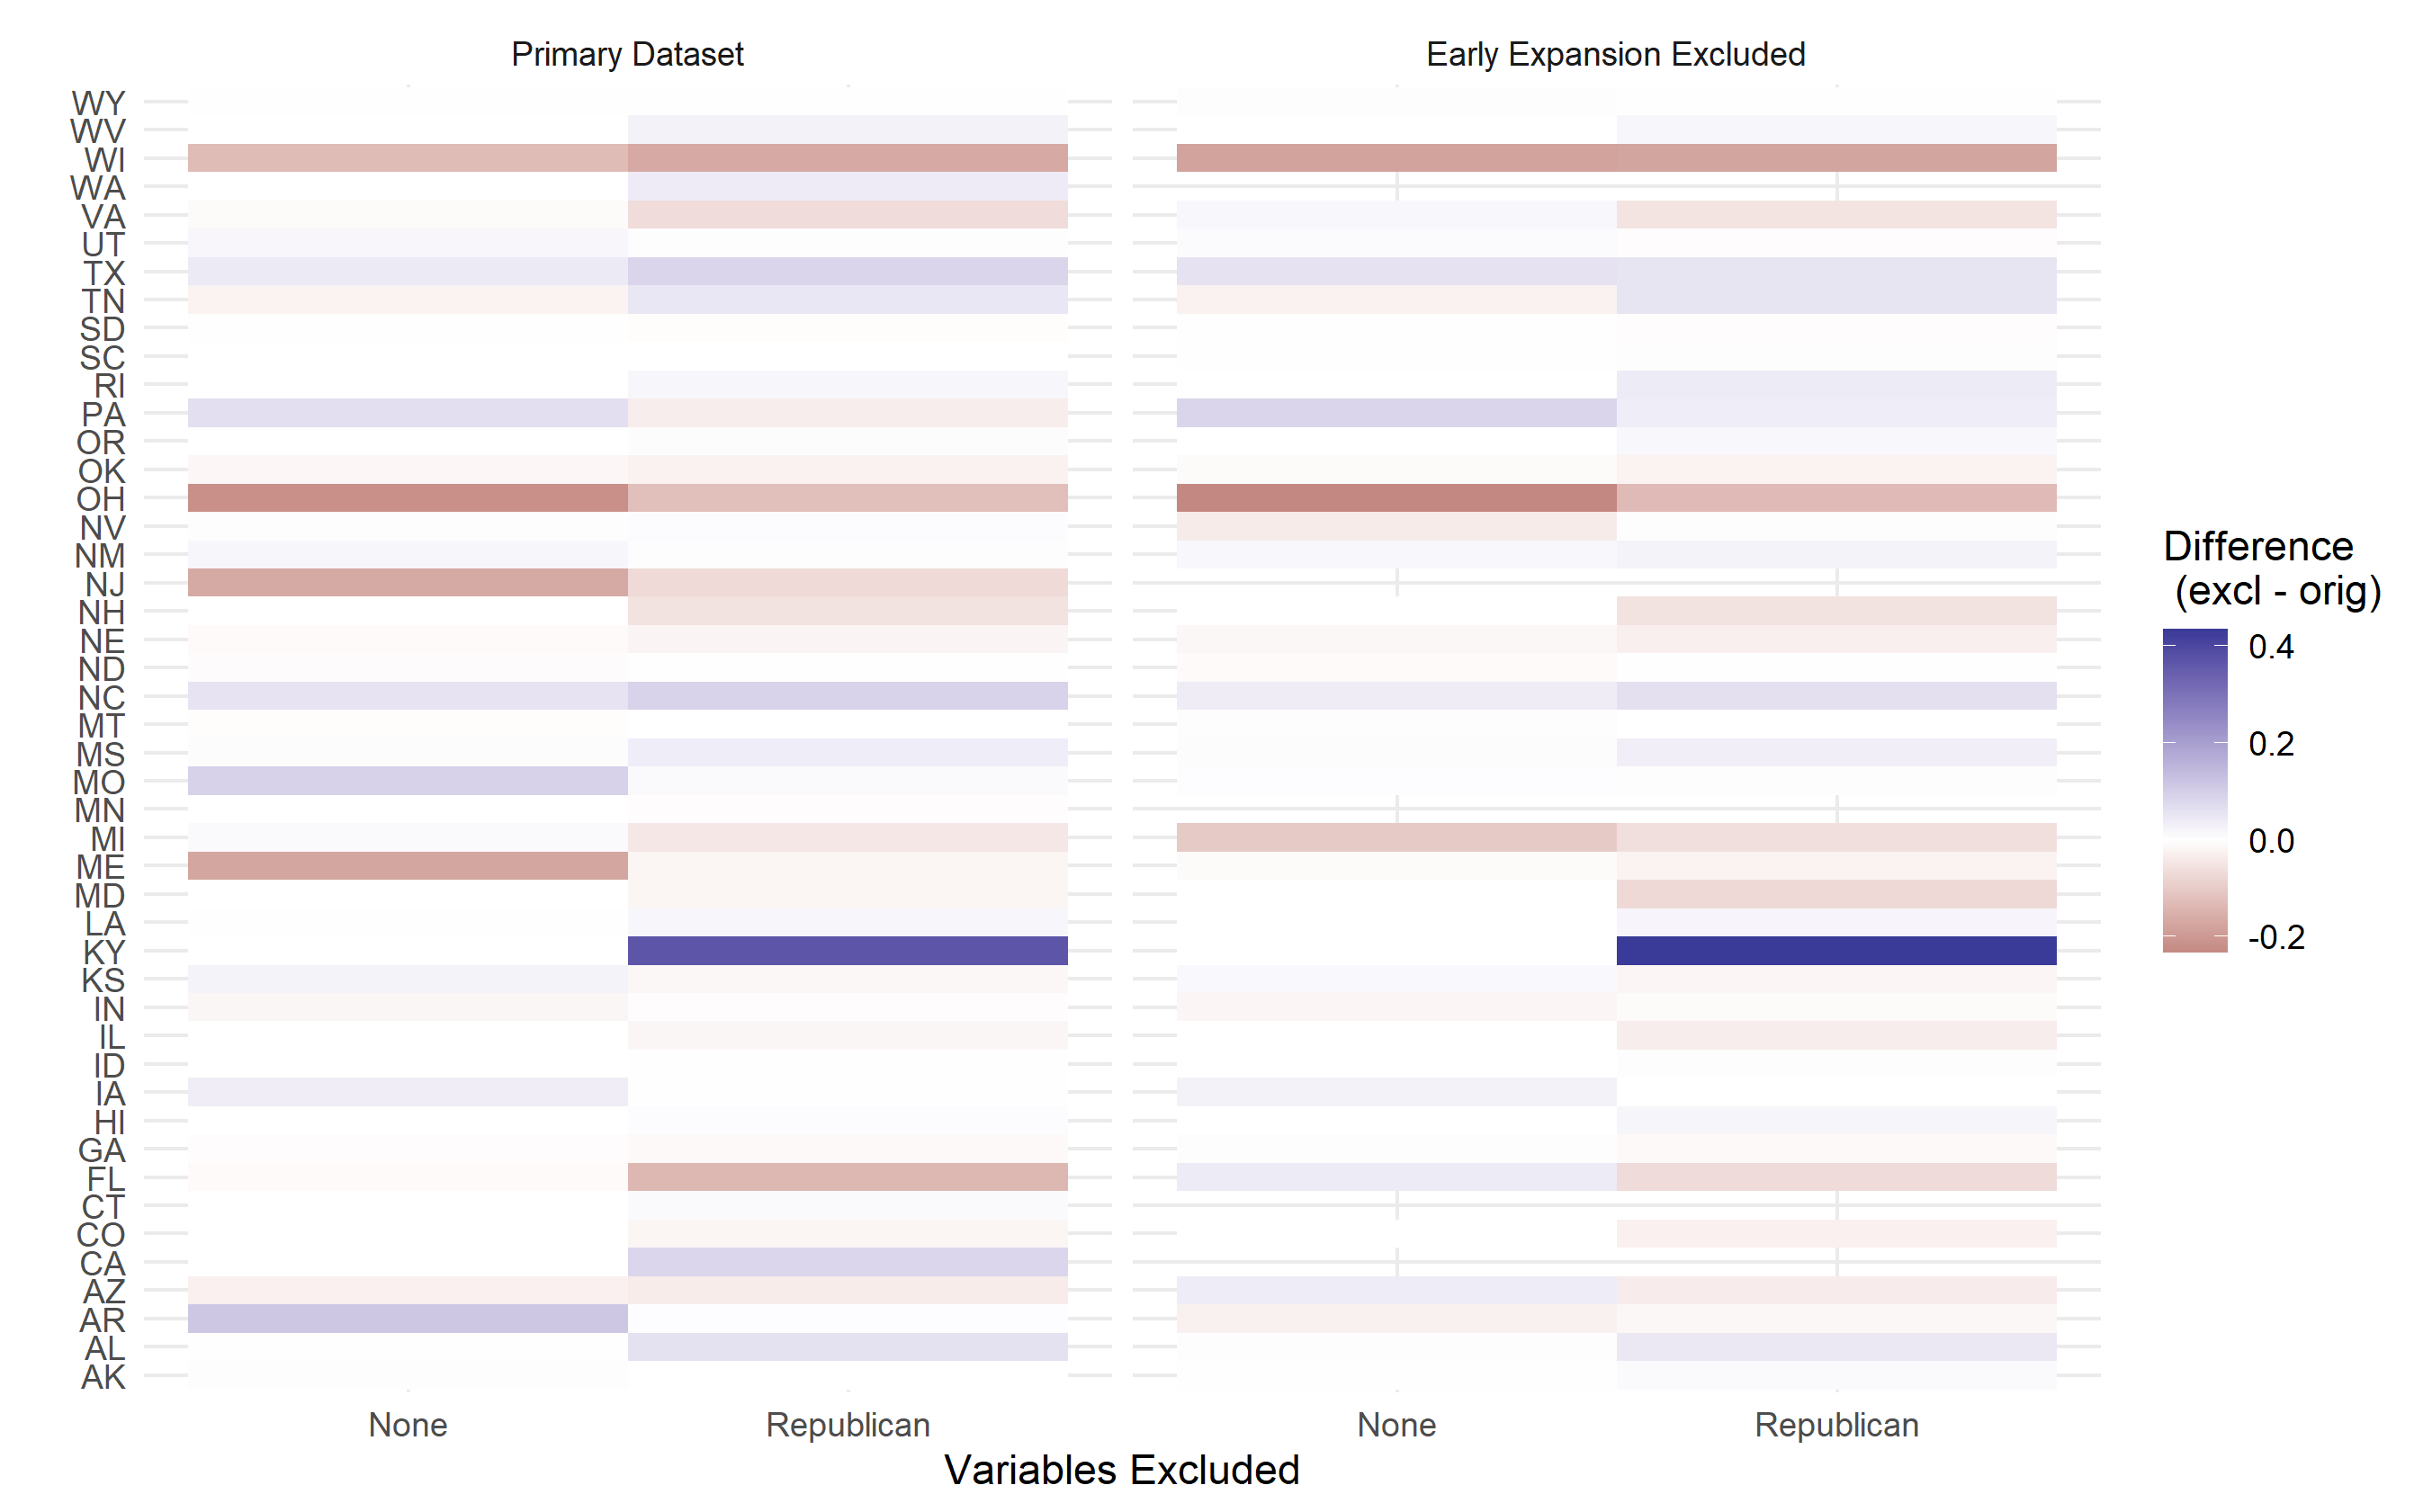
\includegraphics[scale=0.6]{01_Plots/oate-loo-state-cov-group-heatmap-states.png}
\end{center}
\end{figure}

\end{appendix}

%%%%%%%%%%%%%%%%%%%%%%%%%%%%%%%%%%%%%%%%%%%%%%
%% Support information (funding), if any,   %%
%% should be provided in the                %%
%% Acknowledgements section.                %%
%%%%%%%%%%%%%%%%%%%%%%%%%%%%%%%%%%%%%%%%%%%%%%
\section*{Acknowledgements}

The authors gratefully acknowledge invaluable advice and comments from Zachary Branson, Dave Choi, Edward Kennedy, Brian Kovak, Akshaya Jha, Lowell Taylor, and Jose Zubizaretta.

%%%%%%%%%%%%%%%%%%%%%%%%%%%%%%%%%%%%%%%%%%%%%%
%% Supplementary Material, if any, should   %%
%% be provided in {supplement} environment  %%
%% with title and short description.        %%
%%%%%%%%%%%%%%%%%%%%%%%%%%%%%%%%%%%%%%%%%%%%%%
\begin{supplement}
Analysis programs and supporting materials are available online at github.com/mrubinst757
\end{supplement}

%%%%%%%%%%%%%%%%%%%%%%%%%%%%%%%%%%%%%%%%%%%%%%%%%%%%%%%%%%%%%
%%                  The Bibliography                       %%
%%                                                         %%
%%  imsart-nameyear.bst  will be used to                   %%
%%  create a .BBL file for submission.                     %%
%%                                                         %%
%%  Note that the displayed Bibliography will not          %%
%%  necessarily be rendered by Latex exactly as specified  %%
%%  in the online Instructions for Authors.                %%
%%                                                         %%
%%  MR numbers will be added by VTeX.                      %%
%%                                                         %%
%%  Use \cite{...} to cite references in text.             %%
%%                                                         %%
%%%%%%%%%%%%%%%%%%%%%%%%%%%%%%%%%%%%%%%%%%%%%%%%%%%%%%%%%%%%%

%% if your bibliography is in bibtex format, uncomment commands:
\bibliographystyle{imsart-nameyear} % Style BST file
\bibliography{research.bib}       % Bibliography file (usually '*.bib')

%% or include bibliography directly:
% \begin{thebibliography}{}
% \bibitem[\protect\citeauthoryear{???}{???}]{b1}
% \end{thebibliography}

\end{document}
